%% NYU PhD thesis format. Created by Jos� Koiller 2007--2008.

%% Use the first of the following lines during production to
%% easily spot "overfull boxes" in the output. Use the second
%% line for the final version.
%\documentclass[12pt,draft,letterpaper]{report}
\documentclass[12pt,letterpaper]{report}

%% Replace the title, name, advisor name, graduation date and dedication below with
%% your own. Graduation months must be January, May or September.
\newcommand{\thesistitle}{Dynamical inference in the Milky Way}
\newcommand{\thesisauthor}{Jo~Bovy}
\newcommand{\thesisadvisor}{Professor David~W.~Hogg}
\newcommand{\graddate}{May 2011}
%% If you do not want a dedication, scroll down and comment out
%% the appropriate lines in this file.
%\newcommand{\thesisdedication}{To my dog Weierstra\ss, with affection.}

%% The following makes chapters and sections, but not subsections,
%% appear in the TOC (table of contents). Increase to 2 or 3 to
%% make subsections or subsubsections appear, respectively. It seems
%% to be usual to use the "1" setting, however.
\setcounter{tocdepth}{1}

%% Sectional units up to subsubsections are numbered. To number
%% subsections, but not subsubsections, decrease this counter to 2.
\setcounter{secnumdepth}{3}

%% Page layout (customized to letter paper and NYU requirements):
\setlength{\oddsidemargin}{.6in}
\setlength{\textwidth}{5.8in}
\setlength{\topmargin}{.1in}
\setlength{\headheight}{0in}
\setlength{\headsep}{0in}
\setlength{\textheight}{8.3in}
\setlength{\footskip}{.5in}

%% Use the following commands, if desired, during production.
%% Comment them out for final version.
%\usepackage{layout} % defines the \layout command, see below
%\setlength{\hoffset}{-.75in} % creates a large right margin for notes and \showlabels

%% Controls spacing between lines (\doublespacing, \onehalfspacing, etc.):
\usepackage{setspace}

%% Use the line below for official NYU version, which requires
%% double line spacing. For all other uses, this is unnecessary,
%% so the line can be commented out.
%\doublespacing % requires package setspace, invoked above

%% Each of the following lines defines the \com command, which produces
%% a comment (notes for yourself, for instance) in the output file.
%% Example:    \com{this will appear as a comment in the output}
%% Choose (uncomment) only one of the three forms:
%\newcommand{\com}[1]{[/// {#1} ///]}       % between [/// and ///].
\newcommand{\com}[1]{\marginpar{\tiny #1}} % as (tiny) margin notes
%\newcommand{\com}[1]{}                     % suppress all comments.

%% This inputs your auxiliary file with \usepackage's and \newcommand's:
%% It is assumed that that file is called "definitions.tex".
% Graphics:
\usepackage[final]{graphicx}
%\usepackage{graphicx} % use this line instead of the above to suppress graphics in draft copies
%\usepackage{graphpap} % \defines the \graphpaper command

%%BIBSTYLE
\usepackage[authoryear]{natbib}
\bibpunct{(}{)}{;}{a}{}{,}

% Indent first line of each section:
\usepackage{indentfirst}

% Fonts and symbols:
\usepackage{amsfonts,amssymb,amsmath}

%% others
\usepackage{url}
\usepackage{aas_macros}
\usepackage{deluxetable}

%%newcommands
%%Latin
\newcommand{\etal}{et~al.}
\newcommand{\eg}{e.g.}
\newcommand{\ie}{i.e.}

%%Figures etc
\newcommand{\figurenames}{\figurename s}
\newcommand{\sectionname}{\S}
\newcommand{\eqnname}{equation}


%%Solar system paper
\newcommand{\unit}[1]{\mathrm{#1}}
\newcommand{\AU}{\unit{AU}}
\newcommand{\unitday}{\unit{d}}
\newcommand{\yr}{\unit{yr}}
\newcommand{\satellite}[1]{\textsl{#1}}
\newcommand{\Gaia}{\satellite{Gaia}}
\newcommand{\KS}{K--S}
\newcommand{\tvector}[1]{\boldsymbol{\vec{#1}}}
\newcommand{\vx}{\tvector{x}}
\newcommand{\vv}{\tvector{v}}
\newcommand{\vxi}{\tvector{x}_i}
\newcommand{\vvi}{\tvector{v}_i}
\newcommand{\va}{\tvector{a}}
\newcommand{\vI}{\tvector{I}}
\newcommand{\vphi}{\tvector{\phi}}
\newcommand{\tuvector}[1]{\boldsymbol{\hat{#1}}}
\newcommand{\rhat}{\tuvector{r}}
\newcommand{\mvector}[1]{\boldsymbol{{#1}}}
\newcommand{\mvtheta}{\mvector{\theta}}
\newcommand{\mvthetae}{\mvector{\theta}_e}
\newcommand{\mvthetaepsilon}{\mvector{\theta}_{\epsilon}}
\newcommand{\mvomega}{\mvector{\omega}}
\newcommand{\mvomegahatk}{\mvector{\hat{\omega}}_k}
\newcommand{\mvDelta}{\mvector{\Delta}}
\newcommand{\dd}{\mathrm{d}}
\newcommand{\setofxv}{\{\vx_i,\vv_i\}}
\newcommand{\setofrv}{\{r_i,v_{r,i}\}}
\newcommand{\ueff}{u_{\mathrm{eff}}}
\newcommand{\rperi}{r_{\mathrm{peri}}}
\newcommand{\rap}{r_{\mathrm{ap}}}
\renewcommand{\angle}{\phi_r}
\newcommand{\anglei}{\phi_{r,i}}
\newcommand{\ff}{f_{\mvtheta}}
\newcommand{\fff}{\tilde{\ff}}
\newcommand{\lnepsilon}{\ln{\epsilon}}
\newcommand{\vperp}{j^2} % note strange definition
\newcommand{\vperpi}{j_i^2}
\newcommand{\gradient}{\mvector{\nabla}_{\!\!\mvomega}}
\newcommand{\wk}{\ensuremath{w_k}}
\newcommand{\nk}{\ensuremath{n_k}}



%%MASERS
\newcommand{\lsr}{LSR}
\newcommand{\vsunlsr}{\ensuremath{v_\odot}}
\newcommand{\vsunlsrx}{\ensuremath{v_{\odot,x}}}
\newcommand{\vsunlsry}{\ensuremath{v_{\odot,y}}}
\newcommand{\vsunlsrz}{\ensuremath{v_{\odot,z}}}
\newcommand{\vlsr}{\ensuremath{v_{\mbox{\footnotesize \lsr}}}}
\newcommand{\omegao}{\ensuremath{\Omega_0}}
\newcommand{\Ro}{\ensuremath{R_0}}
\newcommand{\zo}{\ensuremath{z_0}}
\renewcommand{\vec}[1]{\mathbf{#1}} % boldface for vectors
\newcommand{\mm}{\ensuremath{\vec{m}}}
\newcommand{\zerovector}{\ensuremath{\vec{0}}}
\newcommand{\masermean}{\ensuremath{\overline{\vv}}}
\newcommand{\samplemean}{\ensuremath{\overline{\tvector{\mu}}}}
\newcommand{\mmR}{\ensuremath{\overline{v}_R}}
\newcommand{\mmphi}{\ensuremath{\overline{v}_\phi}}
\newcommand{\mmz}{\ensuremath{\overline{v}_z}}
\newcommand{\vvpec}{\ensuremath{\vv_{\mbox{{\footnotesize pec}}}}}
\newcommand{\vpec}{\ensuremath{v_{\mbox{{\footnotesize pec}}}}}
\newcommand{\vvmaser}{\ensuremath{\vv_{\mbox{{\footnotesize maser}}}}}
\newcommand{\eeR}{\ensuremath{\vec{e}_{R}}}
\newcommand{\eephi}{\ensuremath{\vec{e}_{\phi}}}
\newcommand{\eez}{\ensuremath{\vec{e}_{z}}}
\newcommand{\vvRi}{\ensuremath{\vpec_{R,i}}}
\newcommand{\vvphii}{\ensuremath{\vpec_{\phi,i}}}
\newcommand{\vvzi}{\ensuremath{\vpec_{z,i}}}
\newcommand{\vvpeci}{\ensuremath{\vvpec_i}}
\newcommand{\ten}[1]{\mathbf{#1}} % boldface for tensors
\newcommand{\RR}{\ten{R}}
\newcommand{\VV}{\ten{V}}
\newcommand{\WW}{\ten{W}}
\newcommand{\II}{\ten{I}}
\newcommand{\TT}{\ten{T}}
\newcommand{\AAA}{\ten{A}}
\newcommand{\maserdisp}{\ensuremath{\mbox{\boldmath$\sigma$}}}
\newcommand{\vgalx}{\ensuremath{\tilde{v}_x}}
\newcommand{\vgaly}{\ensuremath{\tilde{v}_y}}
\newcommand{\vgalz}{\ensuremath{\tilde{v}_z}}
\newcommand{\normal}{\ensuremath{\mathcal{N}}}
\newcommand{\wishart}{\ensuremath{\mathcal{W}}}
\newcommand{\gammadist}{\ensuremath{\mathcal{G}}}
\newcommand{\trace}{\mbox{Trace}}
\newcommand{\T}{^{\scriptscriptstyle \top}}   % transpose
\newcommand{\offsets}{\ensuremath{\Delta\vx_i, \Delta \vv_i}}
\newcommand{\alloffsets}{\ensuremath{\{\offsets\}}}
\newcommand{\pmsgra}{\ensuremath{\mu_{\mbox{{\footnotesize Sgr A$^*$}}}}}
\newcommand{\vres}{\ensuremath{\tvector{v}_{\mbox{{\footnotesize res}}}}}
\newcommand{\vresi}{\ensuremath{\tvector{v}_{\mbox{{\footnotesize res}}, i}}}
\newcommand{\vgal}{\ensuremath{\tvector{v}_{\mbox{{\footnotesize Gal}}}}}
\newcommand{\vgali}{\ensuremath{\tvector{v}_{\mbox{{\footnotesize Gal}}, i}}}

\newcommand{\vlba}{VLBA}
\newcommand{\vlbi}{VLBI}
\newcommand{\vera}{VERA}
\newcommand{\reid}{R09}
\newcommand{\vc}{V_c}
\newcommand{\mw}{MW}

\newcommand{\ra}{\ensuremath{\alpha}}
\newcommand{\dec}{\ensuremath{\delta}}
\newcommand{\pmra}{\ensuremath{\mu_{\ra}}}
\newcommand{\pmdec}{\ensuremath{\mu_{\dec}}}
\newcommand{\eqx}{\ensuremath{x_{\textnormal{eq}}}}
\newcommand{\eqy}{\ensuremath{y_{\textnormal{eq}}}}
\newcommand{\eqz}{\ensuremath{z_{\textnormal{eq}}}}
\newcommand{\gall}{{\it l}}
\newcommand{\galb}{{\it b}}
\newcommand{\pmll}{\ensuremath{\mu_\gall}}
\newcommand{\pmbb}{\ensuremath{\mu_\galb}}
\newcommand{\galx}{\ensuremath{x}}
\newcommand{\galy}{\ensuremath{y}}
\newcommand{\galz}{\ensuremath{z}}
\newcommand{\galU}{\ensuremath{U}}
\newcommand{\galV}{\ensuremath{V}}
\newcommand{\galW}{\ensuremath{W}}
\newcommand{\parallax}{\ensuremath{\varpi}}
\newcommand{\radialdist}{\ensuremath{d}}
\newcommand{\vrr}{\ensuremath{v_r}}
\newcommand{\vll}{\ensuremath{v_\gall}}
\newcommand{\vbb}{\ensuremath{v_\galb}}
\newcommand{\vernal}{\ensuremath{\Upsilon}}
\newcommand{\ngp}{\textnormal{NGP}}
\newcommand{\ngpg}{\textnormal{G}}
\newcommand{\ncp}{\textnormal{NCP}}
\newcommand{\ncpp}{\textnormal{P}}
\newcommand{\gc}{\textnormal{GC}}
\newcommand{\gcc}{\textnormal{C}}
\newcommand{\rangp}{\ensuremath{\ra_\ngp}}
\newcommand{\decngp}{\ensuremath{\dec_\ngp}}
\newcommand{\ragc}{\ensuremath{\ra_\gc}}
\newcommand{\decgc}{\ensuremath{\dec_\gc}}
\newcommand{\degree}{^{\circ}}
\newcommand{\matrixleft}{\left[}
\newcommand{\matrixright}{\right]}
\newcommand{\arcsecs}{\textnormal{as}}

%%HERCULES
\newcommand{\apogee}{APOGEE}
\newcommand{\hermes}{HERMES}
\newcommand{\hipparcos}{\emph{Hipparcos}}
\newcommand{\vR}{\ensuremath{v_R}}
\newcommand{\vphihercules}{\ensuremath{v_{\phi}}}
\newcommand{\vo}{\ensuremath{v_0}}
\newcommand{\ro}{\Ro}
\newcommand{\Ab}{\ensuremath{A_b}}
\newcommand{\Rb}{\ensuremath{R_b}}
\newcommand{\Omegab}{\ensuremath{\Omega_b}}
\newcommand{\fdehnen}{\ensuremath{f_{\text{Dehnen}}}}
\newcommand{\sigmaR}{\ensuremath{\sigma_R}}
\newcommand{\rE}{\ensuremath{R_e}}
\newcommand{\Lc}{\ensuremath{L_c}}
\newcommand{\Rs}{\ensuremath{R_s}}
\newcommand{\Rsigma}{\ensuremath{R_{\sigma}}}
\newcommand{\Rolr}{\ensuremath{R_{\text{OLR}}}}


%% Cross-referencing utilities. Use one or the other--whichever you prefer--
%% but comment out both lines for final version.
%\usepackage{showlabels}
%\usepackage{showkeys}


\begin{document}
%% Produces a test "layout" page, for "debugging" purposes only.
%% Comment out for final version.
%\layout % requires package layout (see above, on this same file)

%%%%%% Title page %%%%%%%%%%%
%% Sets page numbering to "roman style" i, ii, iii, iv, etc:
\pagenumbering{roman}
%
%% No numbering in the title page:
\thispagestyle{empty}
%
\begin{center}
  {\large\textbf{\thesistitle}}
  \vspace{.7in}

  by
  \vspace{.7in}

  \thesisauthor
  \vfill

\begin{doublespace}
  A dissertation submitted in partial fulfillment\\
  of the requirements for the degree of\\
  Doctor of Philosophy\\
  Department of Physics\\
  New York University\\
  \graddate
\end{doublespace}
\end{center}
\vfill

\noindent\makebox[\textwidth]{\hfill\makebox[2.5in]{\hrulefill}}\\
\makebox[\textwidth]{\hfill\makebox[2.5in]{\hfill\thesisadvisor\hfill}}
\newpage
%%%%%%%%%%%%% Blank page %%%%%%%%%%%%%%%%%%
\thispagestyle{empty}
\vspace*{0in}
\newpage

%%%%%%%%%%%%%% Dedication %%%%%%%%%%%%%%%%%
%% Comment out the following lines if you do not want to dedicate
%% this to anyone...
%\vspace*{\fill}
%\begin{center}
%  \thesisdedication\addcontentsline{toc}{section}{Dedication}
%\end{center}
%\vfill
%\newpage
%%%%%%%%%%%%%% Acknowledgements %%%%%%%%%%%%
%% Comment out the following lines if you do not want to acknowledge
%% anyone's help...
\section*{Acknowledgements}\addcontentsline{toc}{section}{Acknowledgements}


Hogg

Fr{\'e}d{\'e}ric Arenou, Michael Aumer, Coryn Bailer-Jones, James
Binney, Michael Blanton, Anthony Brown, Daniela Carollo, Ilias Cholis,
Kyle Cranmer, Walter Dehnen, Mulin Ding, Glennys Farrar, Ken Freeman,
Stefan Gillessen, Andrei Gruzinov, Kathryn Johnston, Joe Hennawi, Matt
Kleban, Dustin Lang, Floor van Leeuwen, Yuri Levin, Stephen Levine,
Tom Loredo, Dmitry Malyshev, Phil Marshall, Surhud More, John
Moustakas, Iain Murray, Adam Myers, Bill Press, Mark Reid, Hans-Walter
Rix, Sam Roweis, Erin Sheldon, Michael Strauss, Scott Tremaine, Glenn
van de Ven, David Weinberg, Neal Weiner, and a few anonymous referees.

Funding agencies: the National Aeronautics and Space Administration
(ADP grant NNX08AJ48G) and the National Science Foundation (grant
AST-0908357). Partial support from the Max-Planck-Institut f\"ur
Astronomie, a New York University Horizon fellowship, and a Horizon
Dissertation writing fellowship. I would also like to acknowledge the
hospitality of The Max-Planck-Institut f\"ur Astronomie and the
Lorentz Center in Leiden.

Software: the HORIZONS System provided by the Solar System Dynamics
Group of the Jet Propulsion Laboratory, the NASA Astrophysics Data
System, and the open-source Python modules scipy, numpy, and
matplotlib.




\newpage
%%%% Abstract %%%%%%%%%%%%%%%%%%
\section*{Abstract}\addcontentsline{toc}{section}{Abstract}
Current and future surveys of the Galaxy contain a wealth of
information about the structure and evolution of the Galactic disk and
halo. Teasing out this information is complicated by measurement
uncertainties, missing data, and sparse sampling. I develop and
describe several applications of generative modeling--—creating an
approximate description of the probability of the data given the
physical parameters of the system--—to deal with these issues.

I develop a method for inferring the Galactic potential from
individual observations of stellar kinematics such as will be
furnished by the upcoming \Gaia\ space astrometry mission. This method
takes uncertainties in our knowledge of the distribution function of
stellar tracers into account through marginalization. I demonstrate
the method by inferring the force law in the Solar System from
observations of the positions and velocities of the eight planets at a
single epoch. I apply a similar method to derive the Milky Way's
circular velocity from observations of maser kinematics.

I infer the velocity distribution of nearby stars from
\hipparcos\ data, which only consist of tangential velocities, by
forward modeling the underlying distribution with a flexible
multi-Gaussian model. I characterize the contribution of several
``moving groups''---overdensities of co-moving stars---to the full
distribution. By studying the properties of stars in these moving
groups, I show that they do not form a single-burst population and
that they are most likely due to transient non-axisymmetric features
of the disk, such as transient spiral structure. By forward modeling
one such scenario, I show how the Hercules moving group can be traced
around the Galaxy by future surveys, which would confirm that the
Milky Way bar's outer Lindblad resonance lies near the Solar radius.

\newpage
%%%% Table of Contents %%%%%%%%%%%%
\tableofcontents

%%%%% List of Figures %%%%%%%%%%%%%
%% Comment out the following two lines if your thesis does not
%% contain any figures. The list of figures contains only
%% those figures included withing the "figure" environment.
\listoffigures\addcontentsline{toc}{section}{List of Figures}
\newpage

%%%%% List of Tables %%%%%%%%%%%%%
%% Comment out the following two lines if your thesis does not
%% contain any tables. The list of tables contains only
%% those tables included withing the "table" environment.
\listoftables\addcontentsline{toc}{section}{List of Tables}
\newpage

%%%%% Body of thesis starts %%%%%%%%%%%%
\pagenumbering{arabic} % switches page numbering to arabic: 1, 2, 3, etc.
%% Introduction. If your thesis has no introduction, or chapter 1 is
%% meant to be the introduction, then comment out the lines below.
\section*{Introduction}\addcontentsline{toc}{section}{Introduction}
In the current understanding of the formation of structure in the
Universe the initial tiny density fluctuations are generated during an
inflationary epoch. The dominant mass component---the dark
matter---starts to cluster under the influence of gravity after the
dark matter decouples from the other constituents of the early
Universe, while the ordinary matter of atoms and everyday life remains
coupled to radiation until about 300,000 years after the Big
Bang. When the temperature of the Universe drops below about 3,000 K,
ordinary matter decouples from radiation and falls into the potential
wells created by dark-matter clustering. Ordinary matter is
predominantly found as neutral hydrogen at this stage and this gas
settles at high density at the bottoms of the dark matter
potentials. Stars and later galaxies form in these high density regions.

The current paradigm has been successful in explaining the large-scale
properties of the Universe, especially the close-to-linear regime of
the Cosmic Microwave Background, formed at the epoch of
ordinary-matter--radiation decoupling, and the largest ($> 100 Mpc$
scales in the nearby Universe, where the non-linear influence of
gravity does not play a large role. However, the formation and
evolution of individual galaxies remains to be understood. This is
obvious from the many classes of galaxies and other objects identified
locally (\eg, the Hubble sequence, dwarf Spheroidal galaxies, dwarf
irregular galaxies, etc.) and at higher redshift (\eg, Ultraluminous
infrared galaxies, sub-millimeter galaxies, Lyman-limit systems,
Damped Lyman-$\alpha$ absorbers, MgII absorbers, etc.). How all these
systems form and relate to one another is yet to be explained. 

Since most of Galactic and extra-galactic astronomy is limited to
snapshots at a particular time, one can study the formation and
evolution of galaxies either by looking at galaxies at different
redshifts and interpreting these observations as different stages in
the evolution of present-day galaxies, or one can study galaxies
locally, where observations with much more detail are possible,
especially for the Milky Way and M31, and infer their formation and
evolution. These two approaches move in remarkable lockstep, as the
highest redshifts probed (BOVY: CHANGE) by current and planned surveys
are comparable to the times at which the lowest metallicity stars
currently studied in the Milky Way formed (BOVY: CITE
BLAND+FREEMAN). These approaches are therefore strongly
interrelated. This dissertation focuses on the latter approach.



Absence of major merger for MW (10 Gyr, redshift ?). 


It is known for certain that there is a large amount of dark mass
beyond the Sun’s position in the Milky Way. We expect there to be dark
matter in the inner region of the Galaxy as well. The determination of
the mass distribution in the inner Galaxy, and its decomposition into
the stellar and dark components, is made difficult by the ambiguity of
local stars as tracers of the mass distribution; certain distracting
disk dynamical features such as spiral arms; and our own (moving)
position in the middle of all of this.

While the Milky Way is interesting in its own right—--it is our home
in the Universe--—it is only one among thousands of galaxies in the
local Universe. Despite this, the Milky Way is one of the main sites
for studying structure formation in the Universe on small scales,
because of the amazing amount of detail possible in these
observations. For comparison, the apparent size of the Milky Way’s
nearest neighbor, the Andromeda galaxy, is only a few times that of
the full moon; other nearby galaxies are much farther away. Since we
have no reason to believe that the Milky Way is atypical in any
way—--we can detect many galaxies with similar features in the night
sky—the details of the Milky Way’s mass distribution and formation
history also provide a general understanding of how galaxies form.


Since stars move across the sky at a slow pace and because they orbit
the Galaxy on timescales measured in hundreds of millions of years, we
can hope at best to measure their positions and velocities at the
present time, while their accelerations are beyond our observational
reach. This poses a fundamental difficulty for interpreting the data
in terms of the mass distribution that guides them.  Newton’s second
law says that the acceleration of a star is directly set by the force
acting on it, while its velocity merely reflects the initial motion of
the object and not the underlying force. Thus, without the
accelerations of stars it seems that we cannot know the underlying
mass distribution. This problem and its resolution is discussed in
Chapter I.

To derive the mass distribution of the Milky Way from stellar motions,
we need to make additional assumptions about the kinematics of stars
that couple these motions to the mass distribution. One such
assumption is that the distribution of the stellar positions and
velocities is time-independent.  This seemingly simple assumption
provides the coupling between the underlying mass distribution and the
stellar kinematics. As an example, I show that we can determine the
force law in the Solar System from observations of the planets’
positions and velocities at one epoch. The nontrivial part of this toy
data set’s analysis is that one has to model the distribution of the
planets’ positions and velocities in a timeindependent manner while
not introducing extra assumptions. I achieve this by building a full
probabilistic model of the data that introduces extra degrees of
freedom describing the time-independent distribution of the positions
and velocities; these extra degrees of freedom can be integrated over
to obtain the final result for the force law in the Solar System which
is independent of the extra degrees of freedom.

Another application considers not observations of stars directly, but
the light of young stars, reprocessed and amplified by the molecular
gas clouds surrounding them. These masers—--lasers on a cosmic
scale—--can be seen to large distances, and their kinematics can be
measured by radio observatories much more precisely than is possible
for stars with optical telescopes. The current data set of 18 masers
contains much information about the disk’s structure, but the
interpretation of the data again depends on our assumptions about the
distribution of their positions and velocities. By inferring a simple
model in which the velocities of the masers are scattered around a
mean offset from the velocity associated with circular motion, we
obtain this circular velocity at the Sun’s position in the
Galaxy. This tells us directly about the Galaxy’s mass within the
Solar radius. This work has been published (Bovy et al. 2009,
Astrophys. J.  704, 1704). 

Chapter III concerns the available data on the motions of stars in the
Galactic disk. The Hipparcos satellite has accurately measured the
positions and motions of stars close to the Sun, which allows us to
look at their detailed properties. First I reconstruct the local
velocity distribution from these data. The result is complex which one
would not expect if the assumptions—axisymmetry and timeindependence
—introduced in the previous paragraphs were correct (this work has
been published: Bovy et al. 2009, Astrophys. J. 700, 1794). Looking at
the mixture of stars that make up the unexpected complexity, I find
that these stars have not formed together such that the complexity is
not due to a formation-history time-dependence and axisymmetry must be
broken. By considering how consistently we can measure the Sun’s
motion relative to the local circular velocity (measured in chapter
II)—--Assuming axisymmetry, this measurement is possible—--I find that
the disk is non-axisymmetric at the level of a few percent.

%% If your thesis has different "Parts", use commands such as the following:
%\part{First Part\label{part:one}}%
\newcounter{tableone}

\chapter[Dynamical inference from a kinematic snapshot: The force law in the Solar System]{Dynamical inference from a kinematic snapshot:\\
  The force law in the Solar System\protect\footnote{Iain~Murray, David~W.~Hogg}\label{chap:solarsystem}}

%\begin{abstract}
%If a dynamical system is long-lived and non-resonant (that is, if
%there is a set of tracers that have evolved independently through many
%orbital times), and if the system is observed at any non-special time,
%it is possible to infer the dynamical properties of the system (such
%as the gravitational force or acceleration law) from a snapshot of the
%positions and velocities of the tracer population at a single moment
%in time. In this paper we describe a general inference technique that
%solves this problem while allowing (1)~the unknown distribution
%function of the tracer population to be simultaneously inferred and
%marginalized over, and (2)~prior information about the gravitational
%field and distribution function to be taken into account. As an
%example, we consider the simplest problem of this kind: We infer the
%force law in the Solar System using only an instantaneous kinematic
%snapshot (valid at 2009 April 1.0) for the eight major planets. We
%consider purely radial acceleration laws of the form $a_r=
%-A\,[r/r_0]^{-\alpha}$, where $r$ is the distance from the Sun.  Using
%a probabilistic inference technique, we infer $1.989<\alpha<2.052$
%(95~percent interval), largely independent of any assumptions about
%the distribution of energies and eccentricities in the system beyond
%the assumption that the system is phase-mixed. Generalizations of the
%methods used here will permit, among other things, inference of
%Milky-Way dynamics from \Gaia-like observations.
%\end{abstract}

\section{Introduction}

The \Gaia~Satellite \citep{Perryman01a} will measure positions and
velocities for millions to billions of stars at varying precision.
One of the principal goals of this mission is to provide the data
necessary to infer the dynamical state of the Milky Way.  However,
there are issues in principle with inference of dynamics from a
\emph{snapshot} or instantaneous set of configuration and velocity
measurements: The instantaneous positions and velocities have no
\emph{necessary} relationship with the gravitational potential or
accelerations.  Indeed, despite a considerable literature \citep[for
  example,][]{Oort32, Schwarzschild79, Little87a, Binney94,
  Johnston99, roulette} there is no methodology for performing this
inference that naturally handles all of the issues, including finite
and non-trivial observational uncertainties or noise, missing data,
non-steady aspects of the mass distribution, and the (incredibly
likely) possibility that the potential is not (simply) integrable.
Robust inference may not even be \emph{possible} if the Milky Way has
significant time-dependence or is strongly chaotic or is far from
showing any simple symmetries (such as axisymmetry).

Certainly there is no hope for dynamical inference on the massive
scale required for the \Gaia\ data set if we can't perform it on much
simpler, much more symmetrical, much older (in a dynamical sense), and
much smaller (in a data sense) systems.  In what follows, we take one
of the simplest possible systems---the Solar System---and the smallest
possible data set---the positions and velocities of the major planets at a
moment in time---and perform a complete dynamical inference.  For a
test system we could also have chosen the black hole at the Galactic
Center, where similar considerations apply.  However, this system has
additional issues with ``missing data'' because not all six
phase-space coordinates are directly measurable for all stars.  The
Solar System truly is the simplest problem in this class.

Our inferential starting point is orbital roulette \citep{roulette}.
In this previous work, it was assumed that the orbital angles (in the
action-angle formalism) are uniformly distributed. Thus, dynamical
model parameters that correspond to orbital angles that suspiciously
lack diversity are rejected. More specifically, the method considers a
large range of possible dynamical model parameters, computes orbital
angles at every value of the parameters, and a distribution statistic
on those orbital angles. If the distribution statistic is designed to
monotonically increase with the diversity of the angles or the
flatness of the angle distribution, the ``best fit'' dynamical model
parameters are those that optimize the distribution statistic.  This
kind of approach is inherently frequentist: on many applications of
these procedures to independent datasets a confidence interval
captures the true dynamical parameters on a guaranteed fraction of
trials. However, for any given dataset the confidence interval
produced might not represent a credible set of parameters.

In what follows we cast the dynamical parameters estimation as a
probabilistic inference problem (a ``Bayesian'' approach). We adopt
the same core assumption as the roulette problem: we assume that the
orbital angles are uniformly distributed. However, in this framework,
we must also construct prior probability distribution functions for
the dynamical model parameters and conditional probabilities of the
data given the model to encode the assumptions of a long-lived and
bound Solar System.  These prior and conditional probability
distributions and the data create posterior probability distribution
functions for all the parameters. We use this new method to infer the
gravitational force law (radial dependence and amplitude).  What is
new here, in the context of Solar System dynamics, is that we perform
this inference with only a snapshot of the kinematic state, that is,
with only the positions and velocities of the planets at a
\emph{single instant of time.}

Of course the kinematic snapshot we employ is, in fact, a set of
initial conditions for a Solar System integration \citep{Giorgini96a}.
These initial conditions were determined not by a single measurement
at a single epoch, but are in fact the result of an optimization of a
Solar System integration to observed planetary positions over many
decades.  In the context of this paper---a demonstration of a
method---it is best to think of these ``data'' as ``simulated data''
useful for testing the method.  They just happen to be data that have
been simulated by the analog computer we know as the Solar System.

What is new here, in the context of dynamical inference, is that our
method is fully probabilistic or Bayesian.  This is important for
future problems, such as the \Gaia\ problem, or for inferring the mass
of the black hole at the center of the Milky Way, because in these
real data analysis problems, the data points come with non-trivial and
highly correlated observational uncertainties, and because entire
dimensions of phase space are missing or unobserved.  At the Galactic
Center, we do not know the radial distance to anything accurately, and
in the \Gaia\ data set many of the radial velocities will not be
measured.  The Bayesian framework handles these real-world data issues
very naturally, although in fact they are \emph{not} important in the
test problem we solve here.  Aside from these issues of principle, it
is also the case, as we will show, that the Bayesian method performs
extremely well.

Of course, a lot is known about the gravitational force law in the
Solar System, so we don't expect, at the outset, to be surprised by
our results.  The first force-law inference in the Solar System
\citep[][and also work by contemporaries, particularly Hooke, who may
  have priority]{Newton} made use of full orbit shape determination
\citep{Kepler}.  In this sense, Newton's problem---find the force law
(from among a small, discrete group of possible force laws) that leads
to elliptical orbits with the Sun at one focus---was much easier than
the problem we have set for ourselves.  Of course, along the way,
Newton had to develop for the first time the general principles of
kinematics and dynamics!

\section{Parameterized force law, or dynamical model}\label{sec:model}

We are going to assume spherical symmetry of the Solar System's force
law and gravitational potential, although nothing in the general
inference formalism that follows will require this.  Consider a radial
force law (really acceleration law) of the form
\begin{equation}
\va = -A\,\left[\frac{r}{r_0}\right]^{-\alpha}\,\rhat \quad,
\end{equation}
where $A$ is an amplitude, $r$ is the distance from the Sun, $r_0$ is
a distance scale (in this case we will use $r_0=1\,\AU$ so that $A$
can be thought of as the acceleration at the Earth's orbit), $\alpha$
parameterizes the radial dependence, and $\rhat$ is the radial
direction.  In this model, the list of free parameters is
\begin{equation}
\mvomega \equiv \{\ln A,\alpha\}\quad,
\end{equation}
where we have taken the logarithm of $A$ because in inference
problems, dimensioned parameters are usually best handled in the log
\citep{Jeffreys39a,Sivia06a}.

The potential $u$ (potential energy per unit planet mass), radial
effective potential $\ueff$, and binding
energy per unit mass $\epsilon\equiv -E/m$ are
\begin{equation}
u(r) = \frac{A\,r_0}{1-\alpha}\,\left[\frac{r}{r_0}\right]^{1-\alpha} \quad,
\end{equation}
\begin{equation}
\ueff(r) = u(r) + \frac{j^2}{2\,r^2} \quad,
\end{equation}
\begin{equation}
\epsilon = - \ueff - \frac{1}{2}\,v_r^2 \quad,
\end{equation}
where $j^2$ is the square of the magnitude of the planet's angular
momentum per unit mass (or $L^2/m^2$), and $v_r$ is the radial
component of the velocity (the component of $\vv$ parallel to
$\vxsolar$).  The perihelion and aphelion distances $\rperi$ and
$\rap$ are both found by setting $\epsilon=-\ueff$.  With these, we
can define a radial asymmetry $e$
\begin{equation}
e \equiv \frac{\rap - \rperi}{\rap + \rperi} \quad,
\end{equation}
where we have called this ``$e$'' because in the Kepler--Newton
$\alpha=2$ case it is the orbital eccentricity.  One way of thinking of
this radial asymmetry is that at any point in the space made up of the
dynamical parameters $\mvomega$ and the binding energy $\epsilon$,
the radial asymmetry $e$ is a dimensionless description of the
angular momentum magnitude.

Importantly for what follows, we can define a ``radial angle''
$\angle$ that increases linearly with time from perihelion passage
through next perihelion passage.  Any planet at radius $r$ on an orbit
with perihelion distance $\rperi$ and aphelion distance $\rap$ can be
assigned this angle $\angle$ by
\begin{equation}
\angle \equiv \left\{\begin{array}{cl}\displaystyle
  \pi\,\frac{t(r)-t(\rperi)}{t(\rap)-t(\rperi)} & \mbox{for $v_r > 0$}
  \\[2.5ex] \displaystyle
  \pi+\pi\,\frac{t(r)-t(\rap)}{t(\rperi)-t(\rap)} & \mbox{for $v_r < 0$}
\end{array}\right. \quad,
\end{equation}
where the first numerator is the time it takes to go from $\rperi$ to
$r$ outbound, the first denominator is the time it takes to go from
$\rperi$ to $\rap$ outbound, the second numerator and denominator are
the times inbound, and all time differences between two radii can be
computed numerically for general values of $\alpha$ by integrating the
inverse of the radial velocity between these radii. The first-order
form of this integral has an integrable singularity at the perihelion
and aphelion, which can be handled by an appropriate change of
variables \citep[\eg, ][]{Press07a}. A planet observed at a set of
random times spanning many orbits will be observed to have radial
angles $\angle$ drawn from a flat distribution in the range
$0<\angle<2\,\pi$.  This radial angle is one of the angles in the
action-angle formulation of the system, which is integrable for the
simple reason that it is spherically symmetric.

\section{Kinematic data}

In what follows, we are going to use and compare several methods for
inferring the force-law parameters $\mvomega$ (the amplitude $\ln A$
and radial exponent $\alpha$ of the spherical force law) from an
instantaneous snapshot of the positions and velocities of the eight
major planets.  This snapshot was taken from JPL's HORIZONS System
which provides highly accurate ephemerides for Solar System
objects\footnote{Available at \url{http://ssd.jpl.nasa.gov/?horizons}}
\citep{Giorgini96a}. It is an extrapolation (at the time of writing)
to 2009 April 1.0, approximately 400 years after the important
publication of Kepler (1609). This kinematic snapshot is given in
Table~\ref{table:eph}.

Since this snapshot is obtained by integrating the positions and
velocities of Solar System bodies, the accuracy is limited by (i) the
correctness of the dynamical model used, (ii) the numerical
integration of the equations of motion, and (iii) the accuracy to
which the initial conditions are known. It is generally believed that
the dynamical model used is correct and complete, and that the
numerical integration is sufficiently accurate. The main uncertainty
in the ephemerides is then that due to the uncertainty in the initial
conditions. The current set of initial conditions
\citep[DE405;][]{Standish98a} is a fit to a set of optical, radar, and
VLBI observations as well as to a set of spacecraft range and Doppler
points from various space missions. The uncertainties are the largest
for the outer planets, since the data for these are almost entirely
from optical observations (with the exception of Jupiter), and because
Neptune has not been observed over a full orbit since the start of
precise measurements. A comparison between the DE405 ephemerides and
more recent observations shows that the positions of the inner planets
are known to a fractional accuracy of approximately $10^{-8}$, while
those of the outer planets are known to a fractional accuracy of
$10^{-6}$ to $10^{-7}$ \citep{Standish04a}. Uncertainties in the
velocities are at the same fractional magnitude.

This kinematic snapshot is not, of course, a fair data set with which
to perform the inference below, for the main reason that the
``measured'' kinematic state of the Solar System is in fact the output
of fitting observations with a dynamical model that \emph{assumes}
$\alpha=2$.  For this reason, the data should be thought of as
``idealized'' or ``simulated data'' and the work must be considered a
test of the method rather than a definitive inference.

\section{Bound, virialized, and long-lived}

The virial theorem relates the time averages $\left<T\right>$ and
$\left<U\right>$ of a test particle's kinetic and potential energies
through
\begin{equation}\label{eq:virialtheorem}
\left<T\right> = \frac{1-\alpha}{2}\,\left<U\right> \quad,
\end{equation}
where $\alpha$ is the exponent in the radial force law.  Given that a
planet's potential energy is a function of the dynamical parameters
$\mvomega$, while its kinetic energy is not, the virial relation for
each planet becomes a one-dimensional locus in the $\mvomega$ space.
Using kinetic and potential energies computed from the observations as
a proxy for the time-averaged energies, these loci are shown in
\figurenames~\ref{fig:virial_main} and \ref{fig:virial_zoom}.  The
fact that all eight lines cross near a single point in the space is
encouraging that the system is virialized (as we expect) and that the
inference will work. That the eight lines so nearly intersect in a
single point is because, in fact, many of the planets are on circular
orbits; the probabilistic method developed in this paper does not
assume this, but it does retain the precision that is possible because
of this situation.

Also shown in \figurenames~\ref{fig:virial_main} and
\ref{fig:virial_zoom} is the region of parameter space in which one or
more of the planets is unbound because $T>U$ or, equivalently,
$\epsilon < 0$.  In what follows, we will assign vanishing probability
to regions of parameter space in which one or more planets is
unbound. However, as we will see, this does not affect any of our
conclusions. Also shown in \figurename~\ref{fig:virial_main} is the
region of parameter space in which one or more of the planets has
$\rperi<R_\odot$, where $R_\odot$ is the radius of the Sun.  This part
of parameter space ought also to be excluded, although in practice
this is not necessary for any of what follows.

In preparation for what follows, we pre-compute all of the planet
radial angles $\anglei$---given their positions $\vxsolar_i$ and
velocities $\vv_i$---as a function of the dynamical parameters.  These
angles are shown in \figurename~\ref{fig:anglesPlanets}.

\section{Frequentist orbital roulette}\label{sec:freq}

In orbital roulette \citep{roulette}, the idea is to compute, for each
point $\mvomega$ in parameter space, the $N$ radial angles $\anglei$
and analyze them statistically for being well mixed.  In practice,
this means applying a distribution test or multiple distribution tests
to the angles and preferring parameters for which these tests are more
consistent with a random or flat distribution of angles in the range
$0<\angle<2\,\pi$.  Because each test provides one constraint, and in
the case described here the parameter space is two-dimensional, at
least two qualitatively different tests are required to make localized
constraints in $\mvomega$.  In addition to a test for flat angle
distribution we also apply a test for an angle-energy correlation.

About the simplest consistency test for the calculated angles is a
test of the mean of the angles: Is the mean consistent with the
expected mean for a uniformly distributed set of $N$ planets? For this
to perform well one must fold the angles of the inbound planets onto
the interval $[0,\pi]$, that is, disregard the information in the
\emph{sign} of the radial velocity; then the expected mean of the
angles is equal to $\pi/2$ (for details on how to test this
assumption, see \citealt{roulette}). The fact that we have to perform
this mapping indicates that the procedure is \textit{ad
  hoc}. Indeed, for a uniform distribution on the circle there is no
specific meaning to the perihelion and the aphelion, or to any two
points, such that no real meaning can be attached to the mean of the
angles between two arbitrary points on the circle.

Better, one can test the consistency of the full distribution function
of the angles with a uniform distribution. This could again be done
with the full $[0,2\pi]$ distributed angles or with the folded angles;
the results will depend on this choice. Testing an observed
distribution for consistency with an expected distribution often
involves comparing cumulative distribution functions
\citep{Kolmogorov41a}.  The Kolmogorov--Smirnov (\KS) test is the
simplest in practice, since the distribution of the test
statistic---the maximum difference between the cumulative
distributions---can be approximated by an analytic function
\citep{Stephens70a}. The \KS\ test is by construction most sensitive
to deviations near the median value; this rules out dynamical
parameters at which the planets bunch up at perihelion or at aphelion,
the situation in which about half are at perihelion and half at
aphelion can easily dupe the test.

A statistic can be chosen that is
sensitive to deviations at all values, such as the Anderson--Darling
statistic \citep{AndersonDarling}. However, no approximate analytic
description of the distribution of this statistic exists and in
practice this distribution has to be obtained by Monte Carlo sampling
\citep[\eg, ][]{roulette}. A statistic
more appropriate to the problem at hand (although we
are not primarily interested in a careful examination of the differences
between different frequentist procedures) is Kuiper's
statistic \citep{Kuiper62a}. This statistic---the sum of
the maximum distance of the observed cumulative distribution above and
below the expected cumulative distribution---is invariant under
periodic shifts of the angle and was specifically designed to test
uniform distributions on the circle. The advantage over
Anderson--Darling is that the asymptotic distribution of the
Kuiper statistic is known \citep[\eg, ][]{Press07a}.

All of these tests for the uniformity of the distribution of the angles
are shown in \figurename~\ref{fig:freq}. These tests can fail when for
a certain combination of dynamical parameters some planets are near
aphelion while other planets are near perihelion. This situation
appears here in \figurename~\ref{fig:anglesPlanets},
at $\alpha$ far from $2$, where there are
large regions in which the inner planets, especially Mercury and
Venus, are near perihelion, while the outer planets, especially Uranus
and Neptune, are near aphelion and \textit{vice versa}.  This prevents
the mean angle and \KS\ tests from excluding those regions. The Kuiper
test performs better.

A second constraint (for the two-dimensional parameter space) comes
from a second test. In regions of parameter space in which
the inner planets are all near perihelion and the outer planets are
all near aphelion, a significant correlation between the angles and
the energies exists. This correlation is unphysical if the system is
not being observed at any special time.
A non-parametric test for the correlation is preferred
here as the angle-energy correlation will not in general be linear. We
perform a test of the angle-energy correlation using Kendall's $\tau$
\citep{Kendall38a}.  This is a rank test; it only considers the
relative ordering of the angles and energies of different planets (for
details on this test see \citealt{Press07a}). That this test is in a
sense orthogonal to the tests of the uniformity of the angle
distribution can be seen in \figurename~\ref{fig:freq}.

All of the frequentist tests permit acceptance or rejection of a
dynamical model at a certain confidence level. 95 and 99~percent
confidence intervals for all of the frequentist tests are shown in
\figurename~\ref{fig:freq}. Also shown is the combination of the tests
of the uniformity of the angle distribution with the test of the
angle-energy correlation.

\section{Probabilistic dynamical inference}

The frequentist procedures perform reasonably well in this simple
problem because the number of dynamical parameters is small and the
data have vanishing errors and no missing components. As the number of
dynamical parameters increases the frequentist must find larger
numbers of tests in order to break degeneracies.  While data
uncertainties can be included by sampling the error distribution of
the data and combining the results \citep[\eg, ][]{roulette}, this
will perform badly in the limit of low signal-to-noise or missing
data. These difficulties are related to the fact that these procedures
use only a very crude model of the data, that is, that the angles are
distributed uniformly and that angle-energy correlations should be
absent, which allows no room for discovery of structure in phase
space. A fully Bayesian treatment of this problem can treat the
phase-space distribution function as an unknown function to be
inferred from the data. Modeling the full phase-space distribution
function permits simultaneous inference of missing data and properly
marginalized probability distributions for dynamical parameters.

Imagine that we have the three-vector positions $\vxsolar_i$ and
three-vector velocities $\vv_i$ at some time $t$ for $N$ planets $i$
and a parameterized model for the gravitational acceleration law
(force law per unit mass) $\va_{\mvomega}(\vxsolar)$, a function of
position $\vxsolar$ and a list of parameters $\mvomega$.  We wish to
obtain an estimate of the posterior probability distribution
$p(\mvomega|\setofxv)$ for the parameters, where $\setofxv$ is the set
of all planet positions and velocities.  We employ Bayes's theorem as
follows:
\begin{equation}\label{eq:bayes}
p(\mvomega|\setofxv) = \frac{p(\setofxv|\mvomega)\,p(\mvomega)}{p(\setofxv)} \quad,
\end{equation}
where, as usual, $p(\setofxv|\mvomega)$ is the likelihood or the
probability distribution function for the data given the model
parameters, evaluated at the observed values of the data,
$p(\mvomega)$ is the prior probability distribution function for the
parameters, and the denominator is (for our purposes here) a
normalization constant.

For our chosen parameterization of the dynamical parameters,
$\mvomega$, a broad flat or uniform prior in the space represents a
reasonable description of our (assumed) prior knowledge.  The much
more challenging problem is to specify the likelihood of the dynamical
parameters, the conditional probability distribution function
$p(\setofxv|\mvomega)$. Without detailed knowledge of how the Solar
System formed, this probability distribution is also a representation
of our prior beliefs. Ideally our ability to learn from the observed
data will not be too sensitive to these beliefs.

It is easier to express beliefs about the angle~$\phi_r$, radial
asymmetry~$e$, and binding energy~$\epsilon$ of each planet than its
position and velocity. This is because, given our assumption that the
planets constitute an angle-mixed population, Jeans's theorem
\citep{Jeans15a,binneytremaine} tells us that the distribution
function, which is proportional to the probability of observing a
planet at a certain locus in phase space, is only a function of the
integrals of the motion. We wish to assign zero probability to
dynamical parameters that lead to any of the computed binding energies
$\epsilon(\vxsolar_i,\vv_i,\mvomega)$ being negative (because we defined
$\epsilon > 0$ to be bound). We would also like to expresses our prior
information or assumption that the system is long-lived (in units of
the dynamical time), that it is non-resonant, and that we are not
seeing the system at any special time, or that the radial angles
$\angle$ will be randomly distributed between $0$ and $2\,\pi$. In the
absence of any better information, we will try to be as agnostic as
possible about the \emph{actions} (conserved quantities) of the
planets but extremely confident that all radial angles
$0<\angle<2\,\pi$ are equally likely.

In the simple spherical or radial situation under consideration here,
in which there are no missing data, we can rewrite the likelihood as a
function of the planets' radial coordinates, as the orientation of the
orbit does not depend on the dynamical parameters:
\begin{equation}
p(\vxsolar,\vv|\mvomega) \propto p(r,v_r,\vperp|\mvomega) =
|J(\lnepsilon,e,\angle;r,v_r,\vperp)| \;p(\lnepsilon, e,
\angle|\mvomega) \quad .
\end{equation}
where, again, we have gone to $\lnepsilon$ because dimensioned
parameters are usually best handled in the log, and
$J(\lnepsilon,e,\angle;r,v_r,\vperp)$ is the Jacobian matrix of all
the partial derivatives of $(\lnepsilon,e,\angle)$ with respect to
$(r,v_r,\vperp)$. For spherical potentials, this Jacobian is given by
\begin{equation}\label{eq:jacgeneral}
|J(\lnepsilon,e,\angle;r,v_r,\vperp)| = \frac{2\,\pi}{T_r}\,\frac{1}{\epsilon}\,\left|\frac{\partial e}{\partial \vperp}\right|,
\end{equation}
where the derivative is evaluated at the current location in phase
space and $T_r$ is the radial period, which depends on the dynamical
parameters and the integrals of the motion. For general $\alpha$ this
radial period can be computed numerically (see
\sectionname~\ref{sec:model}). The derivative of the radial asymmetry
with respect to the specific angular momentum squared can be written
in terms of the perihelion and aphelion distance as
\begin{equation}\label{eq:dedj2}
\frac{\partial e}{\partial \vperp} = A r_0^{\alpha}\,\rap\, \rperi
\frac{\rap^{3-\alpha} - \rperi^{3-\alpha}}{(\rap+\rperi)^2}\,
\left[\vperp-A r_0^3\left(\frac{\rap}{r_0}\right)^{3-\alpha}\right]^{-1}
\left[\vperp-A r_0^3\left(\frac{\rperi}{r_0}\right)^{3-\alpha}\right]^{-1}\,.
\end{equation}
In the special case $\alpha = 2$ this Jacobian is
\begin{equation}\label{eq:jacobian}
|J(\lnepsilon,e,\angle;r,v_r,\vperp)| \propto \epsilon^{3/2}\,e^{-1}\,M_{\odot}^{-3}\,
\end{equation}
where we have dropped any terms that do not depend on the mass of the
Sun.

As well as assuming that the angles are independently and uniformly
distributed, we might further assume that the energy and radial
asymmetry of each planet was drawn independently:
\begin{equation}
    p(\{\lnepsilon_i, e_i, \anglei\}|\mvomega) =
    \frac{1}{(2\pi)^N}
    \prod_{i=1}^N p(e_i,\lnepsilon_i|\mvomega)\quad.
\end{equation}
However, a priori we do \emph{not} know the distribution function from
which radial asymmetries and binding energies were drawn. Fixing
$p(e_i,\lnepsilon_i|\mvomega)$ to a broad distribution would be making
a strong assumption: regardless of what the data say we would continue
to dogmatically believe that the distribution function was broad,
which could result in poor inferences about the model as a whole.

We can assume that the planets' properties were drawn independently
and identically distributed, without making strong assumptions about
what that distribution was. This is achieved by introducing auxiliary
parameters $\mvtheta = \{\mvthetae, \mvthetaepsilon\}$ that if known
would specify the distribution function. Since we do not know these
nuisance parameters, introducing a prior $p(\mvtheta|\mvomega)$ and
marginalizing over them,
\begin{equation}
    p(\{\lnepsilon_i, e_i, \anglei\}|\mvomega) = \frac{1}{(2\pi)^N}
    \int \dd\mvtheta \;\, p(\mvtheta|\mvomega) \prod_{i=1}^N p(e_i,\lnepsilon_i|\mvtheta,\mvomega)\quad,
\end{equation}
is then part of the inference task. With all of this in place, we
apply \eqnname~(\ref{eq:bayes}) to get the posterior distribution
over the dynamical parameters
\begin{equation}
p(\mvomega | \setofxv) \propto 
  \left[\prod_{i=1}^N |J(\lnepsilon_i,e_i,\anglei;r_i,v_{r,i},\vperpi)|\right] \,
  \int\dd\mvtheta\;p(\mvtheta,\mvomega)
  \,\prod_{i=1}^N
  \,p(e_i,\lnepsilon_i|\mvtheta,\mvomega)\quad ,
  \label{eqn:posterior}
\end{equation}
where each planet's value of $(\lnepsilon_i,e_i,\anglei)$ is a
function of phase-space position $(\vxsolar_i,\vv_i)$ and dynamical
parameters $\mvomega$, and the Jacobian is evaluated at each planet's
value of $(\lnepsilon_i,e_i,\anglei)$.

For situations in which we have missing data or noisy observations,
further unknown quantities will be added to the model and marginalized
over. As the model becomes more complicated it is more likely that
Markov chain Monte Carlo \citep[\eg,][]{neal1993} or other approximate
computational methods will be required.

\subsection{Basic method}

To keep things as simple as possible, at first we model the
distribution function $p(\lnepsilon, e|\mvomega,\mvtheta)$ as a
product of a top-hat function in $\lnepsilon$ from $\lnepsilon_a$ to
$\lnepsilon_b$ with a top-hat function in $e$ from $e_a$ to $e_b$. In
this context, the phase-space parameter list is
\begin{equation}
\mvtheta = \{ \lnepsilon_a, \lnepsilon_b, e_a, e_b \} \quad.
\end{equation}
In what follows, we only consider values $A <\ln \epsilon_a < \ln
\epsilon_b < B$, where $A$ and $B$ provide very distant
(uninformative) limits (below, we will take the limit), and $0 \leq
e_a \leq e_b \leq 1$. These enforce our assumption or prior
information that the system is bound.

For our initial model we also set the prior $p(\mvtheta,\mvomega)$
flat or uniform in all the parameters. Now the marginalization
required to compute the posterior (equation~\ref{eqn:posterior}), an
integral over all four of the phase-space distribution parameters
in~$\mvtheta$, can be performed analytically; it leaves
\begin{equation}\label{eq:basic_posterior}
\begin{split}
p(\mvomega | \setofxv) \propto\,\,
  & [\lnepsilon_K - \lnepsilon_L]^{2-N}
    \left[1-[1-e_L]^{2-N}-[e_M]^{2-N} + [e_M-e_L]^{2-N}\right]\\
  & \quad\times\prod_{i=1}^N
    |J(\lnepsilon,e,\angle;r_i,v_{r,i},\vperpi)|\quad ,
\end{split}
\end{equation}
where $\lnepsilon_L$ is the lowest planetary binding energy at this
point $\mvomega$ in dynamical parameter space, $\lnepsilon_K$ is the
highest, $e_L$ is the lowest planetary radial asymmetry at this point
$\mvomega$, $e_M$ is the highest, and we have taken the limit in which
the range of the parameters $(\lnepsilon_a,\lnepsilon_b)$ goes to
infinity, or $A \rightarrow -\infty$, $B \rightarrow \infty$. This
posterior probability distribution for $\mvomega$ represents our
posterior beliefs marginalized over all possible values of
$\{\lnepsilon_a,\lnepsilon_b,e_a,e_b\}$ of the tophat model.


\subsection{Alternative methods}
\label{sec:altmethods}

The results of any inference depend both on the data and on modeling
assumptions. Thus, it is always sensible to question any assumptions
and investigate how sensitive the results are to them.

The marginalization in our basic method is tractable at the expense of
believability: it seems unlikely that the true distribution function
over the planet properties is uniform in the chosen
parameterization. If the true distribution function is far from this
assumption, the inference performed here could be in trouble because
the zero prior probability assigned to all other reasonable forms of
the distribution function makes it impossible for the model to learn
this. This family of distribution functions also has no special
status: a distribution which is uniform in one parameterization, will
not be uniform in another. Instead of modeling the distribution in
$(\lnepsilon, e,\angle)$, we could have chosen to model the
distribution function in terms of $(\lnepsilon,e^2,\angle)$. This set
of parameters is, in a sense, more natural as it is closer to
action-angle coordinates, and, thus, the Jacobian
$|J(\lnepsilon,e^2,\angle;r,v_r,\vperp)|$ is more close to
constant. Indeed, from \eqnname~(\ref{eq:jacobian}) it is clear that,
in the case of $\alpha = 2$, this Jacobian does not depend on the
eccentricity of the orbit any longer and
\figurename~\ref{fig:ejacobiansPlanets} shows that this Jacobian is
close to constant for all values of $\ln A$ and $\alpha$. However, it
is not obvious a priori whether using this parameterization will give
better results.  Rather than guessing, we can assume that the
distribution over radial asymmetries is uniform in an unknown
parameterization, and infer from the data what this parameterization
should be. We tried assuming that the radial asymmetry was uniform
over some range of $e$, $e^2$ or $\sqrt{e}$, with equal prior
probability over each choice. This method corresponds to extending
$\mvtheta$ to parameterize a richer class of distributions. As we did
with nuisance parameters before, we can marginalize over this choice.

In general we could marginalize over a very flexible class of
distributions for both the binding energy and radial asymmetry. A
generic way of representing distributions is with a histogram, where
any distribution can be represented within an arbitrary tolerance for
sufficiently narrow bins. Some care is required in putting a prior
$p(\mvtheta)$ over the heights of the bins. It is tempting to use a
Dirichlet distribution, which allows analytical marginalization.
However, this assumes that the heights of the bins are unrelated
except through their overall normalization. An arbitrarily spiky
distribution function is not only unphysical, but we would be unable
to infer its shape from point observations.

We attempted to construct a sensible prior over distributions using
histograms with many bins by coupling the heights of the bins so that
the densities appear smooth. Since the focus on this paper is on the
principles of dynamical inference and not on the specific result on
the Solar System's force law, we only provide a brief description of
how we implemented this approach. We refer the interested reader to
the references provided in the following for more details on the
specifics. A multivariate Gaussian prior can be put over the log bin
heights, approximating a logistic Gaussian process
\citep{leonard1978}. We used 100 equal-width bins coupled with a
Gaussian covariance function \citep{rasmussen2005a}. We put uniform
priors over the start and end points of the histogram and over
physically reasonable ranges of the covariance function's parameters.
The posterior over the dynamical parameters was estimated by Markov
chain Monte Carlo simulation of all the unknowns, Gibbs sampling was
used to update the dynamical parameters over a grid of values for
which we had precomputed the Jacobian term. Slice sampling
\citep{neal2003a} was used to update all nuisance parameters, except
the bin heights which were updated with a Metropolis--Hastings method
\citep[Eq.~15]{neal1999a}.

\section{Results and discussion}

In our basic method we evaluate the Jacobian $|J(\ln
\epsilon,e,\angle;r_i,v_{r,i},\vperpi)|$ for each planet at the
observed radius, radial velocity, and specific angular momentum, for
each value of the dynamical parameters $\mvomega$, and multiply the
magnitudes of the determinants of these Jacobians together. Following
equation (\ref{eq:basic_posterior}) we multiply this product with the
value of the marginalized product of the distribution function and
finally multiply this with the (uniform) prior on the dynamical
parameters in order to obtain the posterior probability distribution
for the dynamical parameters.

It is instructive to look at the magnitude of the determinant of the
Jacobian for each planet as a function of the dynamical parameters in
\figurename~\ref{fig:jacobiansPlanets}. These factors seem to show a
clear preference for the dynamical parameters of each planet to lie on
its virial locus. Why is this? For nearly circular orbits the last two
factors in \eqnname~(\ref{eq:dedj2}) are equal and are unbounded for
perfectly circular orbits; this results in a natural preference for
nearly circular orbits for all of the planets, \ie, for each planet to
lie somewhere along its virial locus. At the same time the measured
non-zero radial velocity limits the extent to which a planet's orbit
can be circularized by a suitable choice of the dynamical parameters
and, thus, how close to the circular singularity an individual planet
can be brought. This naturally leads to a weighting scheme in which
planets that are closer to circular orbits (as measured by the
observed angle between the planet's velocity and the tangent to the
circular orbit going through its present location) receive a higher
weight in the analysis than planets on less circular orbits. This
weighting scheme is good in that planets on more circular orbits are
indeed more informative about the potential than planets on less
circular orbits. Therefore, it may seem that the decision to model the
radial asymmetries as uniform in $e$ was fortuitous, but in fact, as
we will discuss below in \sectionname~\ref{sec:sensitivity}, the
results obtained using the basic method are robust in that more
flexible models learn that the tophat in $e$ leads to a good
interpretation of the data.

The posterior probability distribution is shown in
\figurename~\ref{fig:Bayes2d}. A strong peak is apparent near $\alpha
= 2$ and the Newtonian Solar value for $\ln A$.  The width of the
probability distribution is indicated by the 95 and 99~percent
posterior contours. These contours are defined to enclose the
smallest area that holds 95 and 99~percent, respectively, of the
posterior probability distribution.

In order to infer the exponent $\alpha$ of the force power-law we
perform a second marginalization of the posterior probability
distribution, this time over the (for our purposes) uninteresting
parameter $\ln A$. This gives a posterior probability distribution for
the parameter~$\alpha$
\begin{equation}
p(\alpha|\setofxv) = \int \dd \ln A\, p(\mvomega|\setofxv) \quad.
\end{equation}
This probability distribution is shown in
\figurename~\ref{fig:Bayes1d}. The 95 and 99~percent posterior
intervals in this figure are defined to exclude 2.5 and 0.5~percent,
respectively, of the distribution on either side of the central
region.

The result of the inference is not a value for the parameters but a
posterior probability distribution.  A ``best fit'' value for $\alpha$
could be obtained according to various criteria. For example, the
posterior mean minimizes the expected square difference from the true
parameter. However, since the posterior distribution is multi-modal, a
point-estimate does not capture our uncertainty.  The posterior is
better summarized by a credible interval, containing a given fraction
of the probability mass. The 95~percent posterior interval is $1.989 <
\alpha < 2.052$. This compares favorably with the results obtained by
\citet{Newton} who inferred $\alpha = 2$ from a much richer data set
(though a less rich model set). Modern tests constrain the value of
the exponent $\alpha$ to a fractional accuracy of 10$^{-8}$--10$^{-9}$
on Solar System scales \citep{adelberger,fischbach} using Lunar Laser
Ranging tests \citep{williams} and Keplerian tests comparing $G(r)
M_{\odot}$ and the rate of precession for different planets
\citep{talmadge}.

Our method appears to work well: the true dynamical parameters $A$
and~$\alpha$ are plausible under a fairly tight posterior
distribution, see \figurename~\ref{fig:Bayes2d}. The confidence
intervals from the frequentist tests, \figurename~\ref{fig:freq}, are
somewhat broader than the posterior intervals, but are not directly
comparable. Frequentist confidence intervals do not represent beliefs
about the parameters for this dataset, simply a region that satisfies
some sampling properties. As a result it is unsurprising that the
frequentist confidence intervals appear less good if interpreted as
beliefs given the data. It is difficult to use the frequentist
confidence intervals to make statements about $\alpha$ alone: without
the assumptions of the Bayesian method we cannot marginalize over the
parameter~$A$. One approach that allows frequentist guarantees is to
set $A$ adversarially, but this pessimistic view would give
unreasonably large error bars for~$\alpha$.

That the posterior distribution $p(\alpha|\setofxv)$ turns out to be
multi-modal is no surprise in the light of the virial considerations
from \figurenames~\ref{fig:virial_main} and~\ref{fig:virial_zoom}. The
two peaks in $p(\alpha|\setofxv)$ correspond to the two main
regions in parameter space in which the different virial loci
cross. These virial considerations, and also the frequentist
techniques, are very similar to the probabilistic approach in that
they all prefer each planet to be in a non-special region of radial
angle space, that is, between perihelion and aphelion; this can only
happen simultaneously near the points in parameter space at which
virial loci cross.  The advantage of the probabilistic approach is
that it explains and quantifies this reasoning, and uses it to set
formal limits on the dynamical parameters.

\subsection{Sensitivity analysis}\label{sec:sensitivity}

The strongly peaked Jacobian factors shown in
\figurename~\ref{fig:jacobiansPlanets} depend strongly on the choice
of parameterization. If the model was expressed using the radial
asymmetries squared rather than the radial asymmetries, the Jacobians,
some of which are shown in \figurename~\ref{fig:ejacobiansPlanets},
are much flatter. If the model is maintained by also transforming the
prior over radial asymmetry distributions to the new parameterization,
the posterior distribution over dynamical parameters will be
unchanged. Setting all the radial asymmetries close to one is
penalized elsewhere in the mathematical expression.

However, setting the prior over radial asymmetry distributions to
consider only uniform distributions was a strong assumption. If we had
only considered distributions uniform in the radial asymmetry squared,
this combined with the flat Jacobians in
\figurename~\ref{fig:ejacobiansPlanets} would not have given as tight
a posterior distribution. Fortunately we can infer a suitable
parameterization, or equivalently the distribution function from a
richer family of possibilities, from the data.

\figurename~\ref{fig:altBayes1d} shows the posterior over $\alpha$
from using the two more flexible priors outlined in
\sectionname~\ref{sec:altmethods}. Assuming that the radial asymmetry is
uniform in one of $\sqrt{e}$, $e$ or~$e^2$ gave a 95\% credible
interval of $1.990 < \alpha < 2.035$. A variety of different flexible
priors for the radial asymmetry distribution gave very similar
results.  Allowing the $\ln A$ constant in the force-law to come from
a flexible family of distributions changed the posterior very
little. The 95\% credible interval from the flexible non-parametric
prior on both distributions gave a 95\% credible interval of $1.991 <
\alpha < 2.040$. The fine details of the posterior distribution,
specifically the relative mass in the two modes, are sensitive to
prior assumptions. This is unsurprising with only eight data
points. However, the position of the bulk of the posterior mass, which
gives the confidence interval is surprisingly robust across a wide
range of modeling choices.

As a warning, it is possible to obtain poor results through bad
modeling choices. The reasonable posterior from our basic method,
\figurename~\ref{fig:Bayes1d}, was to some extent due to chance. The
family of possible radial asymmetry distributions is inflexible as it
forces this distribution to be flat over some range in radial
asymmetry. Using the basic method it is not possible to learn the true
distribution, which is not flat in radial asymmetry, from data,
because the truth is assigned zero prior probability. We were
fortunate to choose a parameterization in which the inflexible family
was not too unreasonable. The non-parametric approach is much more
flexible in that its weak smoothness constraints assign non-zero prior
probabilities to all reasonable distribution functions such that the
true one could be picked out with enough data. However, care must also be
taken with non-parametric modeling. An unsmooth Dirichlet prior over
bin heights in a non-parametric prior over distributions gave a broad
and biased distribution over~$\alpha$.

\subsection{Future work}

The necessity of a proper probabilistic approach as laid out in this
paper has been recognized before in the context of inferring the mass
of the Galaxy from a small set of highly informative tracers: distant
satellite galaxies \citep{Little87a} and high velocity stars
\citep{Leonard90a}. The limitations of those works is that they choose
restrictive forms of the distribution function in which the
distribution of angular momentum is fixed as either radial or
isotropic, or given as an inflexible parametric function in
between these two extrema \citep{Kochanek96a}. The precision of their
results for the fundamental parameters of the Galaxy are limited by
the systematic uncertainty arising from this assumption. In the case
of estimating the local escape velocity from a sample of high velocity
stars, a power law model for the energy part of the distribution
function was used; some progress has been made marginalizing over the
exponent, a nuisance parameter, with a prior coming from cosmological
simulations \citep{Smith07a}. In the future, using the technique
introduced in this paper there is no need to make strong assumptions
about the degree of anisotropy of the system at hand or the form of
the distribution function beyond the assumption of complete
angle-mixing. The results of this paper show that by introducing
flexible models for the distribution function that can learn from the
data, robust contraints on the parameters of a dynamical system can be
obtained.

The approach developed here can be applied to other (perhaps more
pressing) dynamical inference problems in which test particles can be
relied upon to be well-mixed in angle space. One such problem is the
dynamics in the region surrounding the black hole at the Galactic
Center. Often in these problems complications arise because of large
observational uncertainties (often highly correlated), the absence of
some of the six-dimensional phase-space coordinates, and selection
effects, all of which are absent in the simple problem considered
here.  It will be necessary for these problems to model the full
six-dimensional phase-space distribution function.  This will
complicate the marginalization over the phase-space parameters, which
was trivial here in the basic method, but at the same time it will
permit the discovery of structure in the phase-space distribution,
which can aid with the presence of missing data and large
observational uncertainties.  That this approach has much potential
has been shown before in the case of the Galactic Center; the
assumption that a set of stars at the Galactic Center is part of a
disk-like population has been successful in reconstructing missing
data \citep{Beloborodov06a}. Extension of the approach developed in
this paper will permit incorporation of much more of the available
data on the dynamics in the central region of the Galaxy.  This, in
turn, will lead to a better determination of the mass of the black
hole and the surrounding density profile.

On larger scales, approaches like that developed in this paper will
prove to be essential for the analysis of the large data sets of
upcoming surveys such as \Gaia. As the duration of the \Gaia\ mission
is vanishingly smaller than any dynamical timescale, the problem posed
is essentially the same as the problem posed here: Infer the dynamics
from a snapshot of the kinematics.  Our approach cannot simply be
applied to this larger problem because the system is almost certainly
\emph{not} (trivially) integrable, and the assumption of mixed angles
and lack of resonances is invalidated by the clear abundance of
substructure in the halo \citep[\eg,
][]{willman,belokurovfield,belokurov,koposov} and the disk
\citep{dehnen98b,Bovy09a}; indeed, Jeans himself, in the paper in
which he first wrote down his eponymous theorem \citep{Jeans15a},
argued \emph{against} assuming a steady state for the Galaxy.
Modeling the details of the phase-space distribution function will be
even more important in this context.  However, we expect that a large
fraction of the Galaxy, even a large fraction of the stellar halo, is
well-mixed, such that mixed-angles approaches are expected to lead to
valuable inferences. Combining the mixed-angle and
unmixed-substructure techniques into a general inference about the
dynamics of the Galaxy requires a fully probabilistic method and the
approach developed in this paper is a baby step towards this ambitious
goal.


\clearpage
\begin{deluxetable}{lr@{.}lr@{.}lr@{.}lr@{.}lr@{.}lr@{.}l}
\rotate
\tablecaption{Planet Ephemerides for 2009-Apr-01 00:00:00.0000 (CT\tablenotemark{\protect{\ref{CT}}})\label{table:eph}}
\tablecolumns{13}
\tablewidth{0pt}
\tablehead{\colhead{Planet} & \multicolumn{2}{c}{$x$} & \multicolumn{2}{c}{$y$} & \multicolumn{2}{c}{$z$} & \multicolumn{2}{c}{$v_x$} & \multicolumn{2}{c}{$v
_y$} & \multicolumn{2}{c}{$v_z$} \\
\colhead{} & \multicolumn{2}{c}{($\AU$)}& \multicolumn{2}{c}{($\AU$)}& \multicolumn{2}{c}{($\AU$)}& \multicolumn{2}{c}{($\AU$ $\yr^{-1}$)}& \multicolumn{2}{c
}{($\AU$ $\yr^{-1}$)}& \multicolumn{2}{c}{($\AU$ $\yr^{-1}$)}}
\startdata
Mercury & 0 & 324190175 & 0 & 090955208 & -0 & 022920510 & -4 & 627851589 & 10 & 390063716 & 1 & 273504997\\
Venus & -0 & 701534590 & -0 & 168809218 & 0 & 037947785 & 1 & 725066954 & -7 & 205747212 & -0 & 198268558\\
Earth & -0 & 982564148 & -0 & 191145980 & -0 & 000014724 & 1 & 126784520 & -6 & 187988860 & 0 & 000330572\\
Mars & 1 & 104185888 & -0 & 826097003 & -0 & 044595990 & 3 & 260215854 & 4 & 524583075 & 0 & 014760239\\
Jupiter & 3 & 266443877 & -3 & 888055863 & -0 & 057015321 & 2 & 076140727 & 1 & 904040630 & -0 & 054374153\\
Saturn & -9 & 218802228 & 1 & 788299816 & 0 & 335737817 & -0 & 496457364 & -2 & 005021061 & 0 & 054667082\\
Uranus & 19 & 930781147 & -2 & 555241579 & -0 & 267710968 & 0 & 172224285 & 1 & 357933443 & 0 & 002836325\\
Neptune & 24 & 323085642 & -17 & 606227355 & -0 & 197974999 & 0 & 664855006 & 0 & 935497207 & -0 & 034716967\\
\enddata
\setcounter{tableone}{1}
\makeatletter
\let\@currentlabel\oldlabel
\newcommand{\@currentlabel}{\thetableone}
\makeatother
\renewcommand{\thetableone}{\alph{tableone}}
\tablenotetext{\thetableone}{\label{CT}
CT is a coordinate time used in connection with ephemeris. It differs from UTC by about 66 seconds (see \url{http://ssd.jpl.nasa.gov/?horizons_doc\#timesys}).\stepcounter{tableone}}
\tablecomments{The $xyz$-coordinate system is defined as follows: the
  $xy$-plane is given by the plane of the Earth's orbit at J2000.0,
  the $x$-axis is out along the ascending node of the instantaneous
  plane of the Earth's orbit and the Earth's mean equator at J2000.0,
  and the $z$-axis is perpendicular to the $xy$-plane in the
  directional (+ or -) sense of Earth's north pole at J2000.0. The
  origin of the coordinate system is given by the barycenter of the
  Solar System. One year is defined as 365.25 days.}
\end{deluxetable}
\makeatletter
\renewcommand{\@currentlabel}{\oldlabel}
\makeatother

\clearpage
\begin{figure}
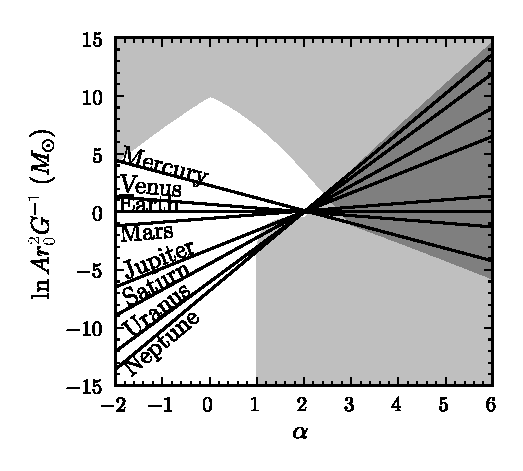
\includegraphics[width=.75\textwidth]{figs_solarsystem/virial_main.ps}
\caption[Virial relation between kinetic and potential energy for each
  of the planets in the Solar System]{The virial relation between the
  kinetic energy and the potential energy
  (equation~[\ref{eq:virialtheorem}]) for each of the eight planets in
  the Solar System. For the combinations of dynamical parameters in
  the light gray region in the lower right at least one planet becomes
  unbound. When the dynamical parameters are in the light gray region
  in the upper left at least one planet has $\rperi<R_\odot$. The
  light gray regions overlap in the dark gray region. In the units
  used in this \figurename, the ``true'' value of $A$ lies at $\ln A
  r_0^2 G^{-1} = 0$.}\label{fig:virial_main}
\end{figure}

\clearpage
\begin{figure}
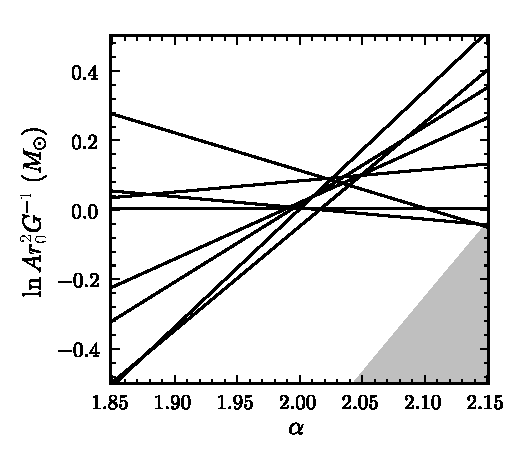
\includegraphics[width=.75\textwidth]{figs_solarsystem/virial_zoom.ps}
\caption{Zoomed in version of \figurename~\ref{fig:virial_main}.}\label{fig:virial_zoom}
\end{figure}

\clearpage
\begin{figure}
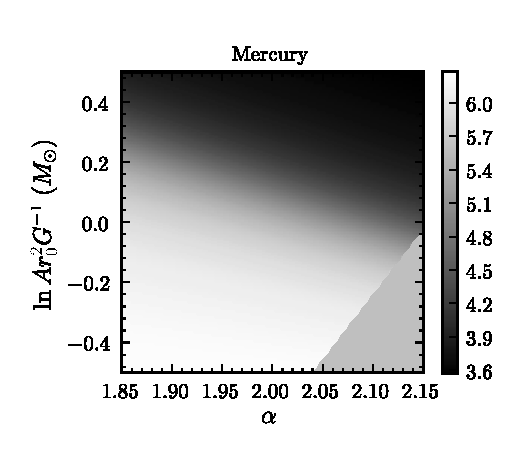
\includegraphics[height=.2\textheight]{figs_solarsystem/phase_Mercury.ps}
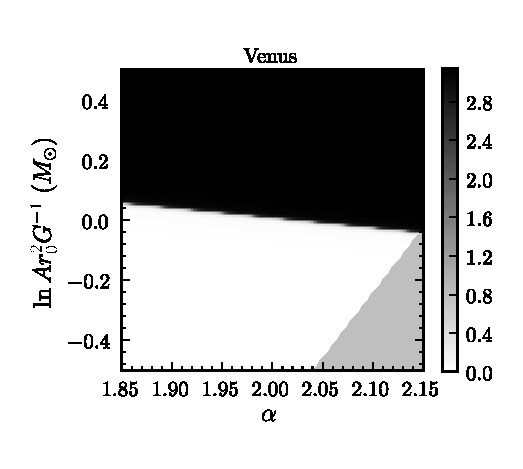
\includegraphics[height=.2\textheight]{figs_solarsystem/phase_Venus.ps}\\
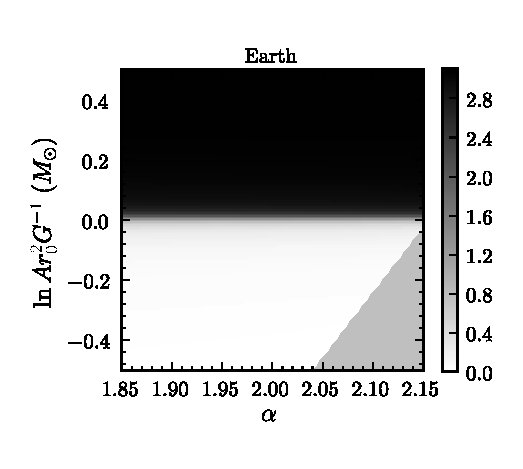
\includegraphics[height=.2\textheight]{figs_solarsystem/phase_Earth.ps}
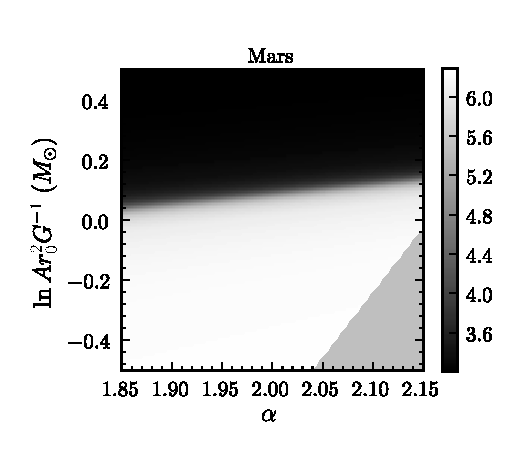
\includegraphics[height=.2\textheight]{figs_solarsystem/phase_Mars.ps}\\
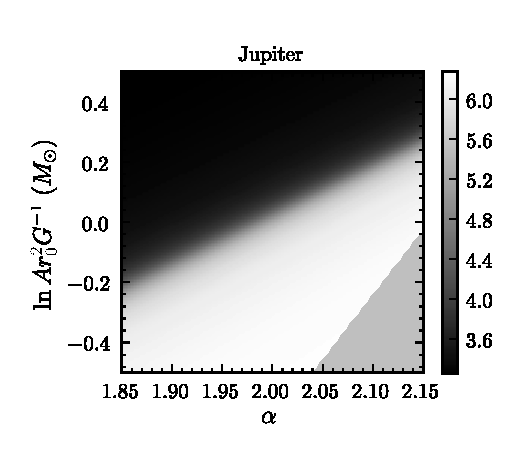
\includegraphics[height=.2\textheight]{figs_solarsystem/phase_Jupiter.ps}
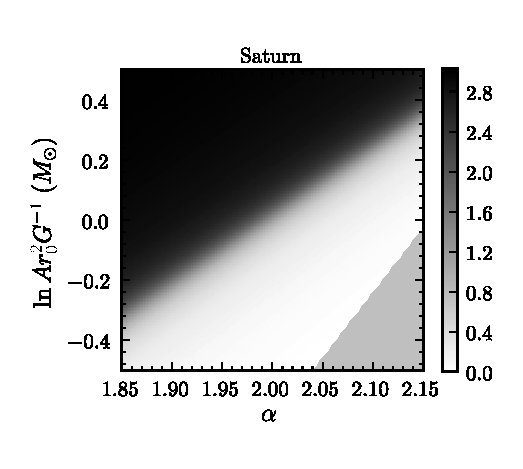
\includegraphics[height=.2\textheight]{figs_solarsystem/phase_Saturn.ps}\\
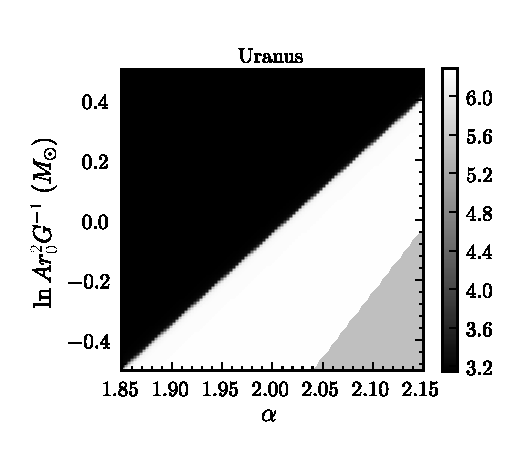
\includegraphics[height=.2\textheight]{figs_solarsystem/phase_Uranus.ps}
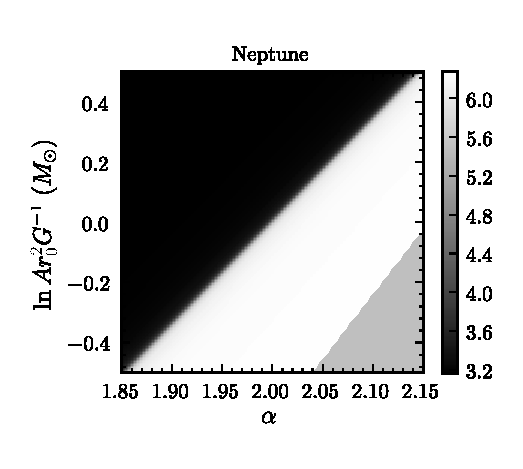
\includegraphics[height=.2\textheight]{figs_solarsystem/phase_Neptune.ps}
\caption[Radial angles for each of the planets as a function of the
  dynamical parameters]{Computed radial angles $\angle$ for each of
  the eight planets as a function of the dynamical parameters. The
  gray triangular region in the bottom-right corner is the region
  excluded by the condition that all the planets are bound.  Each
  planet has an angle range of $0<\angle<\pi$ if it has radial
  velocity $v_r>0$ (outgoing from perihelion) or $\pi<\angle<2\,\pi$
  if it has $v_r<0$ (incoming from
  aphelion).}\label{fig:anglesPlanets}
\end{figure}

\clearpage
\begin{figure}
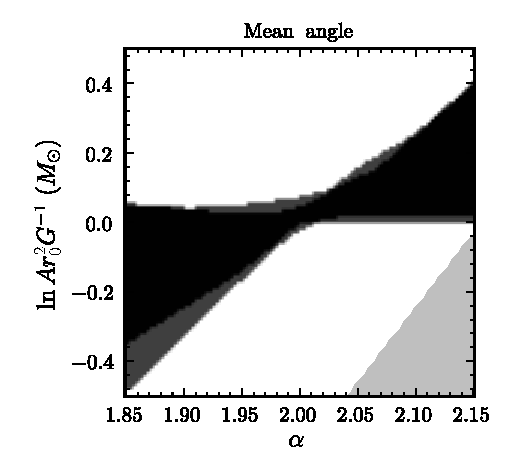
\includegraphics[height=.2\textheight]{figs_solarsystem/freqMean.ps}
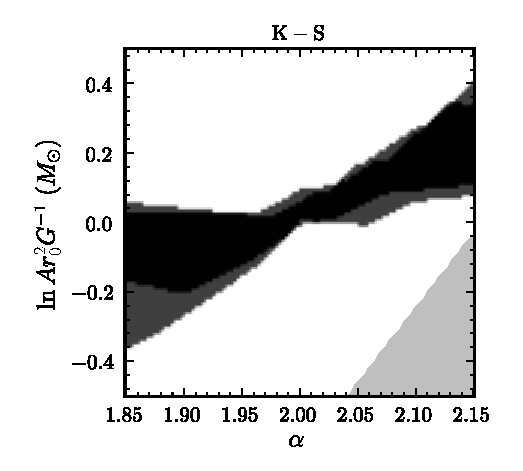
\includegraphics[height=.2\textheight]{figs_solarsystem/freqKS.ps}\\[5pt]
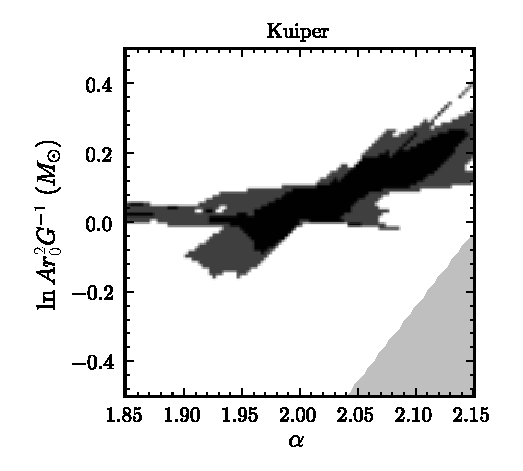
\includegraphics[height=.2\textheight]{figs_solarsystem/freqKuiper.ps}
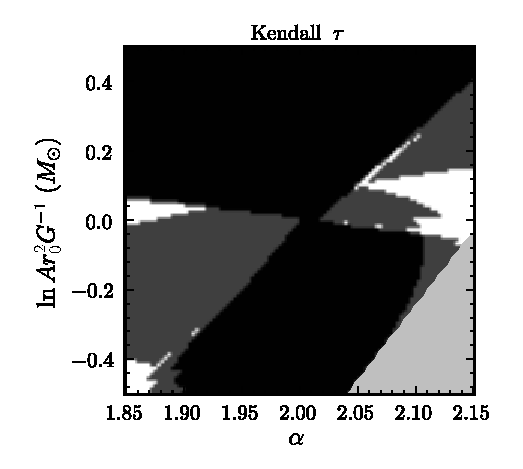
\includegraphics[height=.2\textheight]{figs_solarsystem/freqKendall.ps}\\[5pt]
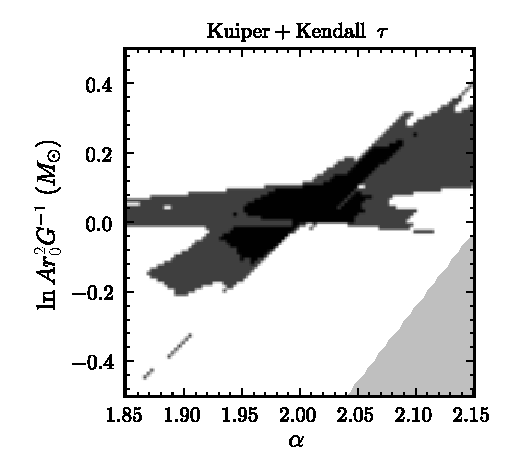
\includegraphics[height=.2\textheight]{figs_solarsystem/freqKuiperKendall.ps}
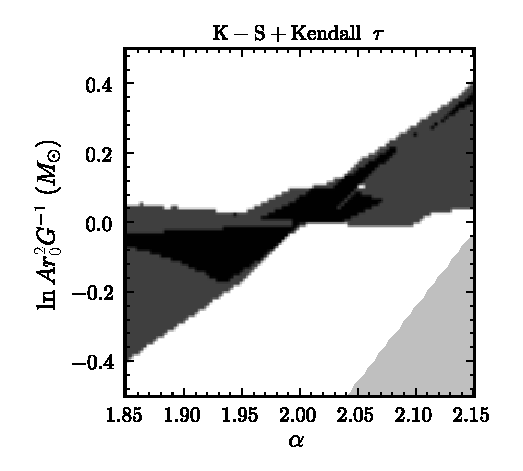
\includegraphics[height=.2\textheight]{figs_solarsystem/freqKSKendall.ps}
\caption[Various frequentist test appied to test the uniformity of the
  angle distribution and the absence of angle-energy
  correlations.]{Various frequentist tests applied to test the
  uniformity of the angle distribution and the absence of angle-energy
  correlations. From top to bottom, left to right: test of the mean of
  the angles; \KS\ test for the uniformity of the angle distribution;
  Kuiper test for the uniformity of the angles; Kendall $\tau$ test
  for the absence of angle-energy correlations; combined confidence
  intervals from the Kuiper test and the Kendall test; combined
  confidence intervals from the \KS\ test and the Kendall test. In the
  plots with a single statistic the darkest region corresponds to the
  95~percent confidence region, the lighter region to the 99~percent
  confidence region. The same is true for the plots with combinations
  of statistics, except that a Bonferroni correction has been applied
  to the significances of the individual statistics that make up the
  combination. In each plot the lightest region is excluded because at
  least one planet becomes unbound for those parameter
  values.}\label{fig:freq}
\end{figure}


\clearpage
\begin{figure}
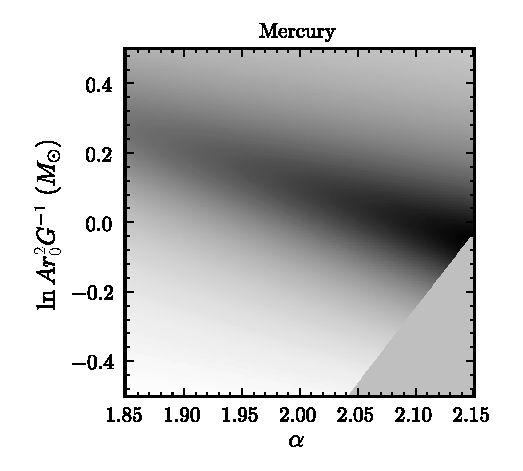
\includegraphics[height=.2\textheight]{figs_solarsystem/jacobian_Mercury.ps}
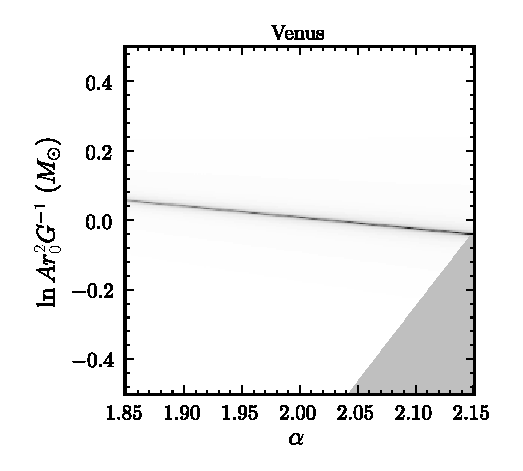
\includegraphics[height=.2\textheight]{figs_solarsystem/jacobian_Venus.ps}\\[5pt]
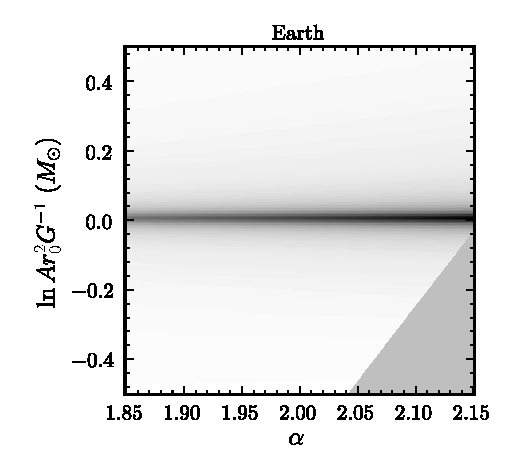
\includegraphics[height=.2\textheight]{figs_solarsystem/jacobian_Earth.ps}
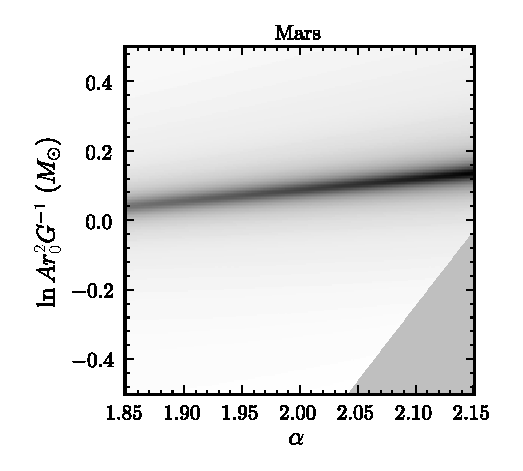
\includegraphics[height=.2\textheight]{figs_solarsystem/jacobian_Mars.ps}\\[5pt]
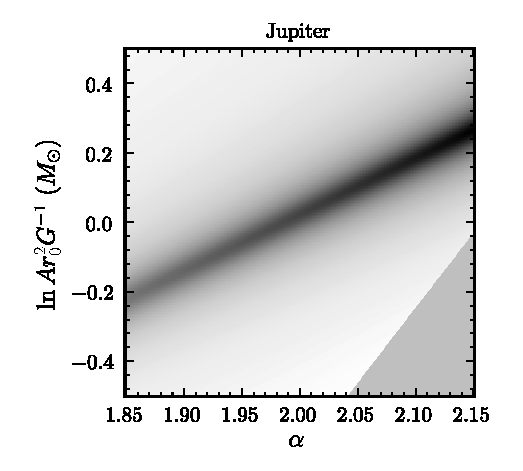
\includegraphics[height=.2\textheight]{figs_solarsystem/jacobian_Jupiter.ps}
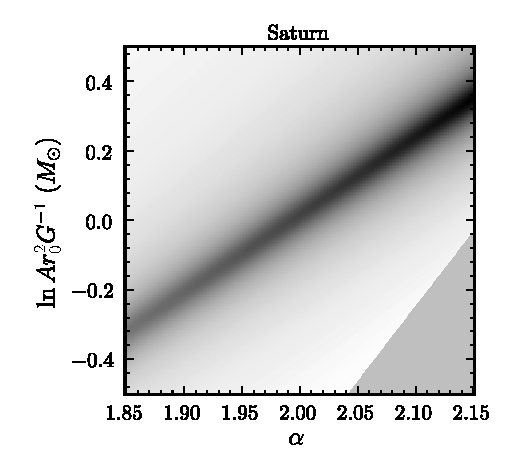
\includegraphics[height=.2\textheight]{figs_solarsystem/jacobian_Saturn.ps}\\[5pt]
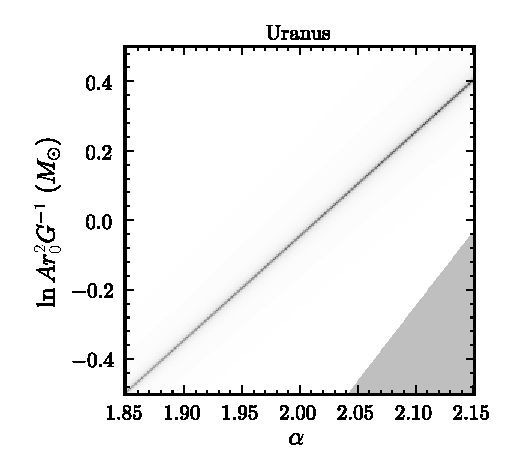
\includegraphics[height=.2\textheight]{figs_solarsystem/jacobian_Uranus.ps}
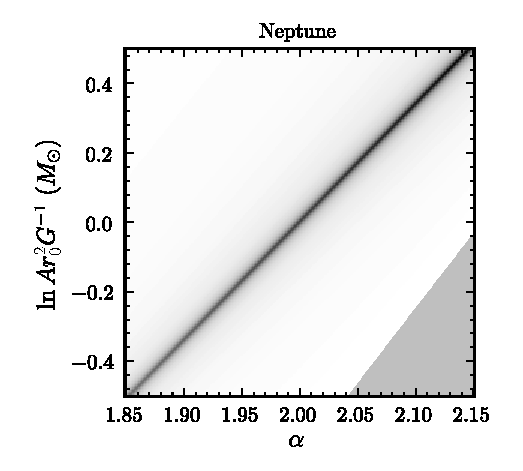
\includegraphics[height=.2\textheight]{figs_solarsystem/jacobian_Neptune.ps}
\caption[Density plots of the absolute value of the determinant of the
  Jacobian of the transformation from the energy, radial asymmetry,
  and radial angle coordinates to the relevant positional and
  kinematical observables]{Density plots of the absolute value of the
  determinant $|J(\lnepsilon,e,\angle;r,v_r,\vperp)|$ of the Jacobian
  of the transformation from the energy $\epsilon$, radial asymmetry
  $e$, and radial angle $\angle$ coordinates to the relevant
  positional and kinematical observables, evaluated at the observed
  positions and velocities of the planets, as a function of the
  dynamical parameters. Grayscales are linear with darker shades for
  larger values.}\label{fig:jacobiansPlanets}
\end{figure}


\clearpage
\begin{figure}
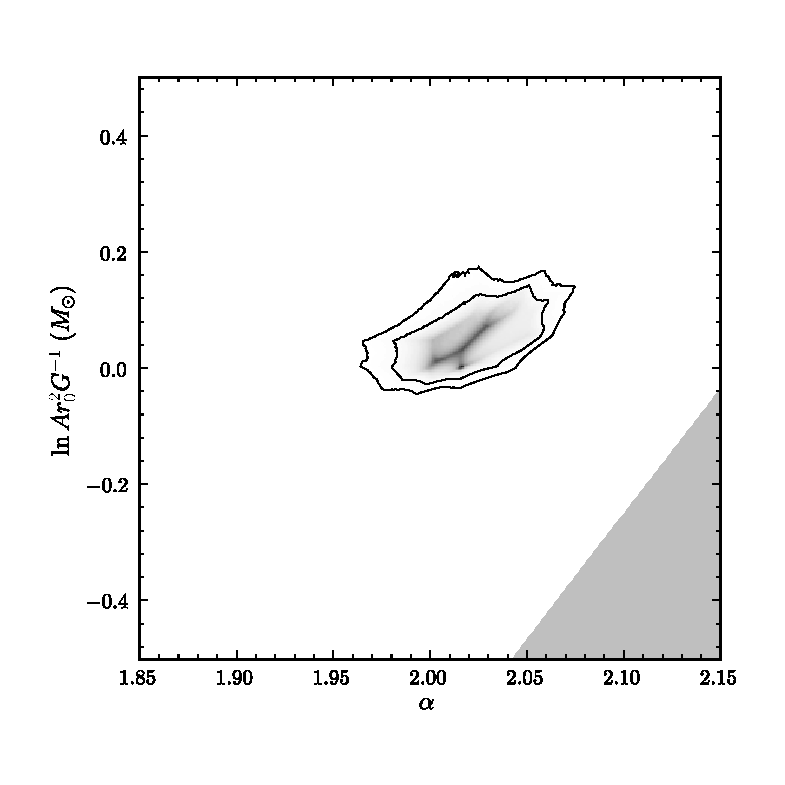
\includegraphics[width=0.6\textwidth]{figs_solarsystem/murrayRoulette.ps}\\%%BoundingBox: 176 285 405 489
\caption[The posterior probability distribution $p(\mvomega|\setofxv)$
  for the dynamical parameters]{The posterior probability distribution
  $p(\mvomega|\setofxv)$ for the dynamical parameters on a linear
  scale. Contours are 95 and 99~percent posterior
  regions.}\label{fig:Bayes2d}
\end{figure}

\clearpage
\begin{figure}
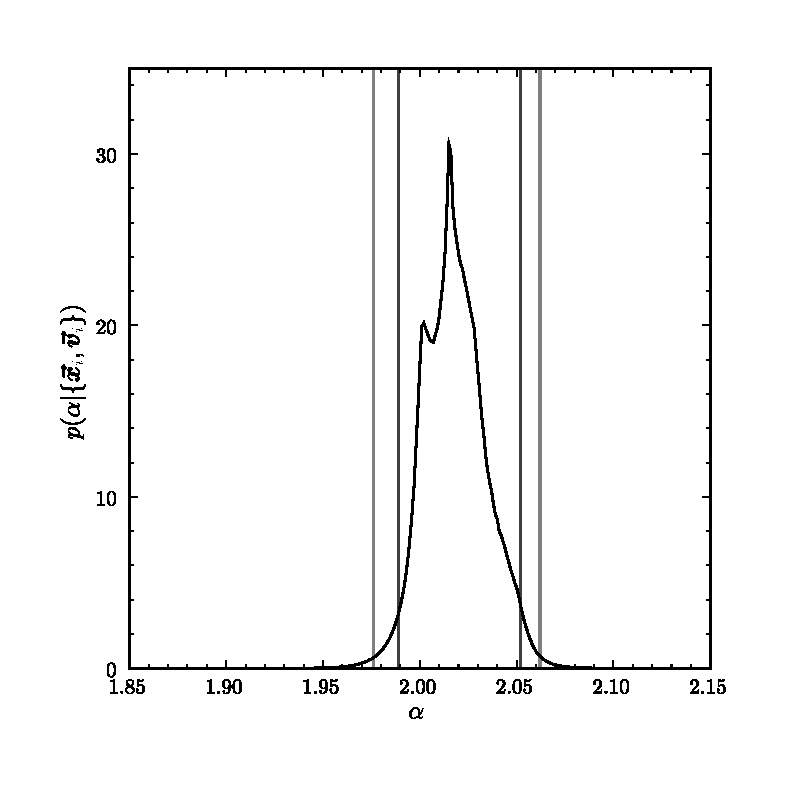
\includegraphics[width=0.6\textwidth]{figs_solarsystem/murrayRouletteAlpha.ps}
\caption{Marginalized posterior probability distribution for the
parameter $\alpha$ with 95 and 99~percent posterior
intervals.}\label{fig:Bayes1d}
\end{figure}

\clearpage
\begin{figure}
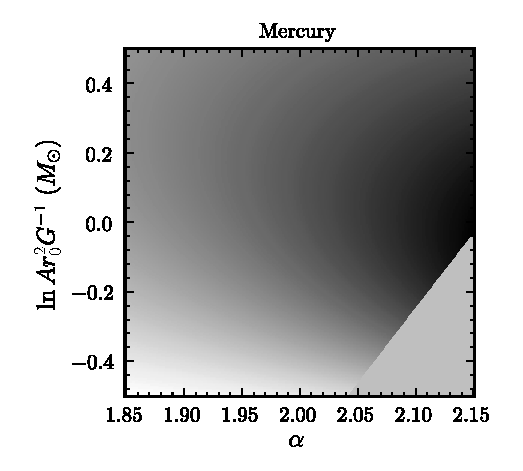
\includegraphics[height=.4\textheight]{figs_solarsystem/ejacobian_Mercury.ps}\\[5pt]
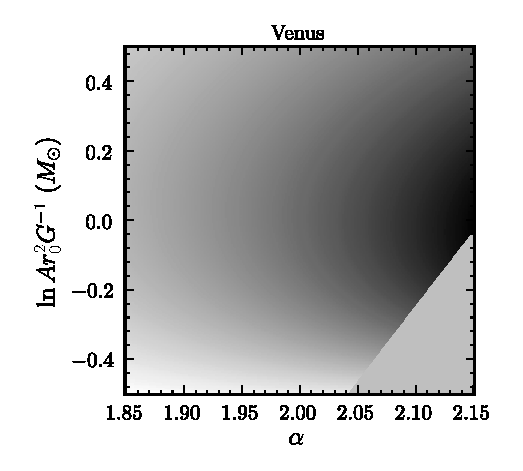
\includegraphics[height=.4\textheight]{figs_solarsystem/ejacobian_Venus.ps}
\caption[Density plots of the absolute value of the determinant of the
  Jacobian of the transformation from the energy, radial asymmetry
  squared, and radial angle coordinates to the relevant positional and
  kinematical observables]{Density plots of the absolute value of the
  determinant $|J(\lnepsilon,e^2,\angle;r,v_r,\vperp)|$ of the
  Jacobian of the transformation from the energy $\epsilon$, radial
  asymmetry squared $e^2$, and radial angle $\angle$ coordinates to
  the relevant positional and kinematical observables, evaluated at
  the observed positions and velocities of the planets, as a function
  of the dynamical parameters. Grayscales are linear with darker
  shades for larger values. Only the Jacobians for Mercury and Venus
  are shown here; the corresponding Jacobians for the other planets
  are very similar to these.}\label{fig:ejacobiansPlanets}
\end{figure}

\clearpage
\begin{figure}
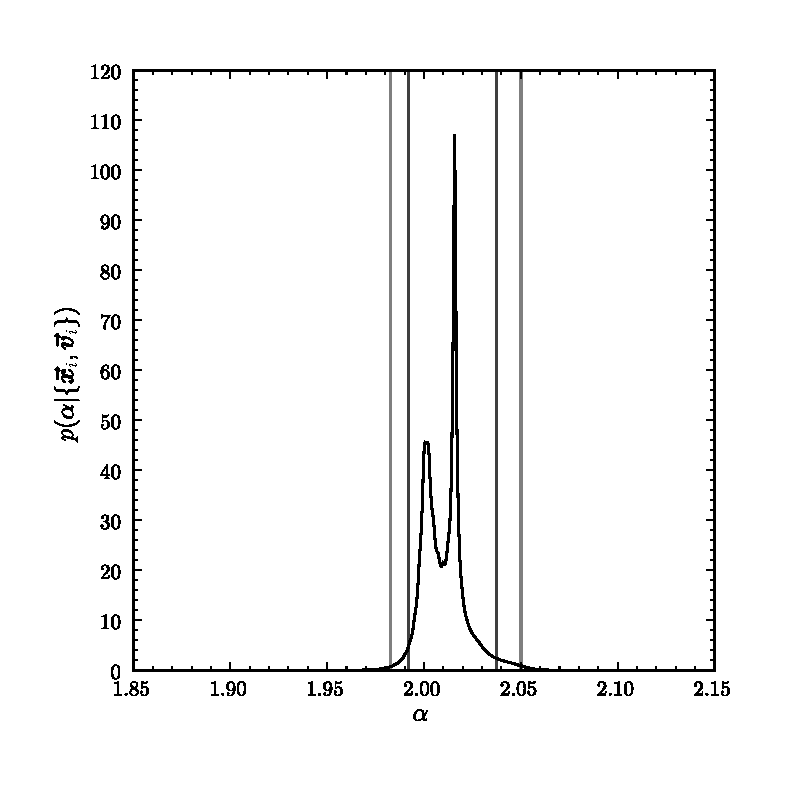
\includegraphics[height=.4\textheight]{figs_solarsystem/alpha_posterior_3es_data6.ps}\\
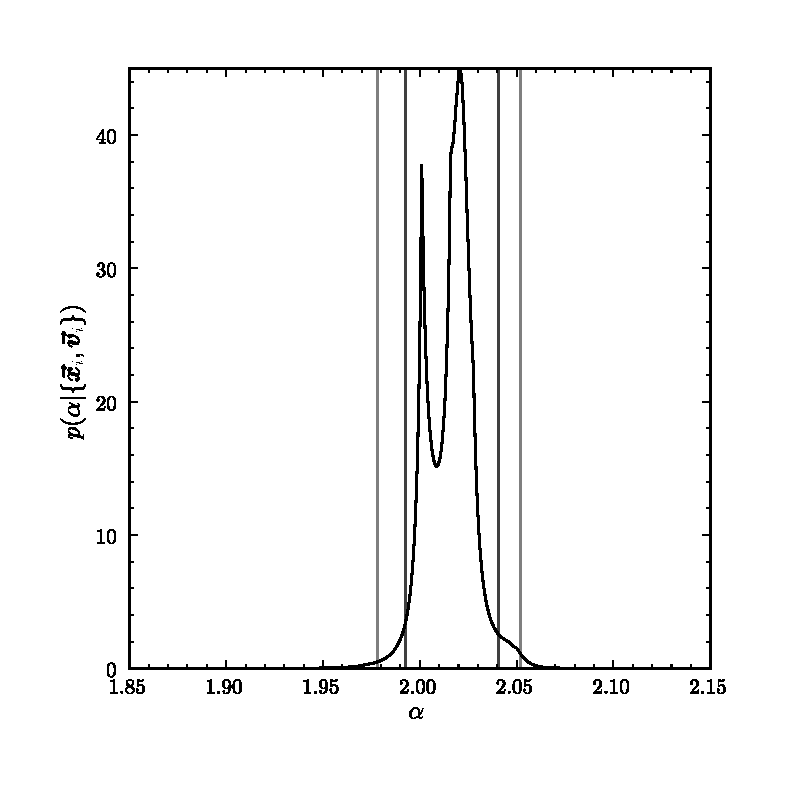
\includegraphics[height=.4\textheight]{figs_solarsystem/alpha_posterior_mcmc_6_500000.ps}
\caption[Alternative posterior probability distributions for the
  parameter $\alpha$]{Alternative posterior probability distributions
  for the parameter $\alpha$ with 95 and 99~percent posterior
  intervals. Top: distribution over radial asymmetry is assumed to be
  uniform in one of $\sqrt{e}$, $e$ or~$e^2$. Bottom: results from a
  non-parametric prior over the distributions of both $e$ and~$\ln
  A$.}\label{fig:altBayes1d}
\end{figure}


\chapter[Galactic masers and the Milky Way circular velocity]{Galactic masers and the Milky Way circular velocity\protect\footnote{Joint work with David~W.~Hogg and Hans-Walter Rix, published as Jo Bovy \etal\ 2009 \emph{ApJ} {\bf 704} 1704. Reproduced by permission of the AAS.}\label{chap:masers}}

\section{Chapter abstract}
Masers found in massive star-forming regions can be located precisely
in six-dimensional phase space and therefore serve as a tool for
studying Milky Way dynamics. The non-random orbital phases at which
the masers are found and the sparseness of current samples require
modeling. Here we model the phase-space distribution function of 18
precisely measured Galactic masers, permitting a mean velocity offset
and a general velocity dispersion tensor relative to their local
standards of rest, and accounting for different pieces of prior
information. With priors only on the Sun's distance from the Galactic
Center and on its motion with respect to the local standard of rest,
the maser data provide a weak constraint on the circular velocity at
the Sun of $\vc = 246 \pm 30$ km s$^{-1}$. Including prior information
on the proper motion of Sgr A$^*$ leads to $\vc = 244 \pm 13$ km
s$^{-1}$.  We do not confirm the value of $\vc \approx 254$ km
s$^{-1}$ found in more restrictive models.  This analysis shows that
there is no conflict between recent determinations of $\vc$ from
Galactic Center analyses, orbital fitting of the GD-1 stellar stream,
and the kinematics of Galactic masers; a combined estimate is $\vc =
236 \pm 11$ km s$^{-1}$. Apart from the dynamical parameters, we find
that masers tend to occur at post-apocenter, circular-velocity-lagging
phases of their orbits.


\section{Introduction}

The value of the circular orbital velocity at the Sun's radius in the
Milky Way is of considerable interest in Galactic and extragalactic
astrophysics. It is necessary to correct observed velocities of stars
and galaxies for the motion of the Sun around the Galactic Center. The
circular velocity also plays a large role in characterizing the mass
of the Milky Way in comparison with other spiral galaxies, placing it
in a cosmological context, \eg, when asking whether the Milky Way
matches the Tully--Fisher relation \citep[\eg][]{Klypin02a,Flynn06a}
or what is its total star formation efficiency
\citep[\eg,][]{Smith07a,Xue08a}.

The circular velocity at the Sun's radius has typically been
established by measuring the Sun's motion with respect to an object
assumed to be at rest with respect to the Galaxy (Sgr A$^*$:
\citealt{Reid04a}; the stellar halo: \citealt{Sirko04a}), or by using
a tracer population assumed to be angle-mixed, \ie, having a uniform
distribution of orbital phases, in a steady-state Galaxy
\citep[\eg,][]{Feast97a}. Recently, a competitive estimate has been
obtained by a different approach using a narrow stellar stream that is
assumed to be tracing out an orbit \citep{Koposov09a}.

In this \chaptername\ we re-analyze a new population of tracers of
Milky Way dynamics: masers associated with star-forming regions
\citep[\reid]{Reid09a}. Using the Very Long Baseline Array (\vlba) and
the Japanese \vlbi\ Exploration of Radio Astronomy (\vera), precise
measurements of the parallaxes, proper motions, and line-of-sight
velocities of masers have been made (see \reid\ and references
therein). These give accurate full six-dimensional phase-space
information in the disk of the Galaxy. Since these massive
star-forming regions are associated with spiral arms and their shocks,
the dense molecular gas regions that produce masers do not lie on
exactly circular orbits, nor are they detected at random points on
their orbits. Therefore, modeling approaches that assume a uniform
distribution of the orbital phases of the tracer population cannot
give accurate determinations of the dynamics of the Galaxy. For the
existing maser data, the problem of non-random orbital phases is
exacerbated by the sparseness of the sample---only 18 masers with
accurate six-dimensional phase-space information have been measured at
present---and by the spatially non-uniform selection of the current
sample of masers.

In this \chaptername, we perform an analysis of the \reid\ maser data
that deals simultaneously with the sparseness of the data, the spatial
non-uniformity of the sampling, the non-random orbital phase
distribution of masers, and prior information. Assuming a flat
rotation curve, $\vc(R) = $ constant, we use a simple model for the
distribution of the maser velocities with respect to their local
standards of rest: a mean offset from circular rotation $\vc(R)$ and a
general velocity dispersion tensor fixed in Galactocentric cylindrical
coordinates. In the probabilistic inference framework that we
use---described in \sectionname~\ref{sec:data}---we can marginalize
over the uncertainty in the inferred distribution function of masers,
take prior information on the dynamics of the Galaxy into account, use
the sparse data set as efficiently as possible, and then ask what
information on $\vc$ the maser data provide. Our results presented in
\sectionname~\ref{sec:results} show that allowing for a finite
velocity dispersion tensor in the model for the maser
peculiar-velocity distribution function leads to lower values of $\vc$
than the large value reported in \reid, in whose analysis the maser
velocity dispersion was (implicitly) assumed to vanish.  Adding in
informative prior information about $R_0$, inferred from monitoring
stellar orbits around the black hole at the center of the Galaxy
\citep{Ghez08a,Gillessen09a} and from the measurement of the proper
motion of Sgr A$^*$ \citep{Reid04a}, we find that the best circular
velocity estimate is $\vc = 244 \pm 13$ km s$^{-1}$, but that the
current maser data set adds little information. We discuss this
measurement and its limitations in the light of other recent
determinations in \sectionname~\ref{sec:discussionmasers}.


\section{Data and methodology}\label{sec:data}

Throughout the analysis that follows we use the standard cylindrical
Galactocentric coordinate frame $(R,\phi,z)$, with associated unit
vectors ($\eeR,\eephi,\eezmasers$) pointing toward the Galactic
center, in the direction of Galactic rotation, and toward the North
Galactic Pole, respectively.

\subsection{Data from \protect\citet{Reid09a}}\label{sec:datasub}

The data we analyze here consist of the Galactic coordinates,
parallaxes, proper motions, and line-of-sight velocities of 18
Galactic masers, as well as their associated uncertainties, presented
in Table 1 of \citet{Reid09a}. Following \reid, we add a 7 km s$^{-1}$
uncertainty in quadrature to the uncertainties in the velocity
components of each maser to describe the random, virial motion in the
massive star-forming region of the individual massive star associated
with each maser.

The line-of-sight velocities have been `corrected' by the radio
observatories' pipelines for the motion of the Sun with respect to the
Local Standard of Rest (\lsr). This correction assumed a value of 20
km s$^{-1}$ toward \ra(B1900.0)= 18$^\mathrm{h}$,
\dec(B1900.0)=$+30\degree$ for the Solar motion \vsunlsr, although it
is unclear whether all observatories used this standard value
(M.~Reid, private communication). We undo this correction, after
which the currently accepted correction for \vsunlsr\ can be applied;
however, as we will describe below, this correction will become part
of our model and, therefore, the correction for \vsunlsr\ does not
occur during the preprocessing of the data.

Beyond these two corrections, no processing of the \citet{Reid09a}
data has been done.


\subsection{Probabilistic framework}

Parameter estimation in a probabilistic framework \emph{by necessity}
uses Bayes's theorem to connect the probability of the model
parameters given the data
$\{\vxi^{\mathrm{obs}},\vvi^{\mathrm{obs}}\}$ to the probability of
the observed data given the model parameters
\citep[\eg,][]{jaynes}. This requires us (1) to identify all the
parameters that need to be included in the model, (2) to write down
the likelihood of the model and (3) to specify suitable priors for the
model parameters. Although the model space needs to be exhaustive, the
probabilistic framework allows integration over uninteresting
parameters.

Here we put forward a model for the maser kinematics in which the
maser velocities are most easily modeled in Galactocentric cylindrical
coordinates. In order to go from the raw data described in
\sectionname~\ref{sec:datasub} to the velocity of each maser in
Galactocentric coordinates, we need to (1) correct the measured
velocity for \vsunlsr, (2) add to this velocity the circular velocity
around the Galactic center at the Sun's radius, and (3) project this
velocity onto the Galactocentric coordinate frame (the details of this
transformation are described in the Appendix of \reid). Since the
latter procedure includes geometrical projection factors depending on
the distance \Ro\ of the Sun from the Galactic Center, the model
parameters need to include the three components of \vsunlsr, \Ro, and
$\vc$. However, it is more practical to assume that Sgr A$^*$ is at
rest with respect to the Galaxy, and to use the proper motion
$\pmsgra$ of Sgr A$^*$ \citep{Reid04a} as a model parameter instead of
the circular velocity, as $\pmsgra$ is very tightly constrained
independently of $R_0$. These two parameters are related simply by
multiplying the proper motion of Sgr A$^*$ by $R_0$ and correcting
this for \vsunlsr. The circular velocity then becomes a parameter
derived from the actual model parameters, which is no problem in the
probabilistic framework, where it is easy to propagate uncertainties
correctly.  As we will assume that the rotation curve is flat, no
extra parameters to model the shape of the rotation curve need to be
included in the model.

If we had uniformly sampled the phase space of masers and full prior
knowledge of the phase-space distribution function of massive
star-forming regions, this would uniquely specify the likelihood of
the model, as the probability of the measured position and velocity of
each maser would simply be given by the distribution function of the
masers convolved with the observational uncertainty. However, we have
neither a uniform sample of masers nor much prior information about
the distribution of masers throughout the Galaxy. To account for the
spatial non-uniformity of the sample we will focus on the distribution
of velocities at the actually observed position of the maser, instead
of using the full six-dimensional phase-space distribution function to
evaluate the likelihood. For this distribution we will assume that it
only depends on the peculiar velocity $\vvpec \equiv \vvmaser - \vc
\cdot \eephi$ of the maser in Galactocentric cylindrical
coordinates. We will assume that this distribution of peculiar
velocities is given by a Gaussian distribution characterized by a
mean, a 3-vector $\masermean$, the offset from circular motion, and a
general velocity dispersion tensor, a symmetric $3 \times 3$ tensor
$\maserdisp$ with six free parameters. Since there have been no
measurements of either the mean offset from circular motion of the
masers or their velocity dispersion, we will use flat priors on these
quantities. This model is essentially a generalization of the model
used in \citet{Reid09a} where the velocity dispersion tensor was
assumed to vanish; this was a poor assumption as we will show below.

The probability of a single maser is thus given by
\begin{equation}\label{eq:onelike}
p(\vxi^{\mathrm{obs}},\vvi^{\mathrm{obs}}|\pmsgra,R_0,\vsunlsr,\masermean,\maserdisp) =
\normal\left(\vvpec[\vx,\vv]|\masermean,\maserdisp\right)\otimes p(\vx,\vv|\vxi^{\mathrm{obs}},\vvi^{\mathrm{obs}})\,,
\end{equation}
where we have suppressed the dependence of $\vvpec$ on the dynamical
parameters, and where the convolution with the observational
uncertainty distribution
$p(\vx,\vv|\vxi^{\mathrm{obs}},\vvi^{\mathrm{obs}})$ has been
included. The posterior distribution for the 14 model parameters is
then given by
\begin{equation}\label{eq:posterior}
\begin{split}
p(\pmsgra,R_0,\vsunlsr,\masermean,\maserdisp|\{\vxi^{\mathrm{obs}},\vvi^{\mathrm{obs}}\})
\propto & \ p(\pmsgra,R_0,\vsunlsr)\\
& \times \prod_i
p(\vxi^{\mathrm{obs}},\vvi^{\mathrm{obs}}|\pmsgra,R_0,\vsunlsr,\masermean,\maserdisp)\,,
\end{split}
\end{equation}
where the first factor on the right-hand side is the prior probability
distribution for these parameters and the product is the
likelihood. We have used flat priors for $\masermean$ and
$\maserdisp$, which is why they do not appear explicitly.

For $\pmsgra$ we use a Gaussian prior with a mean of 30.24 km s$^{-1}$
kpc $^{-1}$ and a standard deviation of 0.12 km s$^{-1}$ kpc$^{-1}$
\citep{Reid04a}. For \Ro\ we combine current state-of-the-art
determinations of \Ro\ from Galactic Center orbits with equal weights:
8.0 $\pm$ 0.6 kpc found by \citet{Ghez08a} and 8.33 $\pm$ 0.35 kpc
found by \citet{Gillessen09a}. This prior is shown as the gray curve
in \figurename~\ref{fig:ro}. For \vsunlsr\ we use the value and
uncertainties obtained from \emph{Hipparcos} data
\citep{2005ApJ...629..268H}, although the clumpiness of the velocity
distribution of nearby stars \citep{1998AJ....115.2384D,Bovyveldist}
implies an uncertainty more on the order of a few km s$^{-1}$ in the
value of \vsunlsr\ (J.~Bovy \& D.~W.~Hogg, in preparation). The
implied prior for the circular velocity is shown as the thick gray
curve in \figurename~\ref{fig:thetao}. To investigate how informative
the maser measurements are about $\vc$ and $R_0$, we will consider the
effect of dropping (some combination of) these priors below.

The framework described here can easily be generalized to more general
descriptions of the distribution of the peculiar velocities of the
masers. In what follows we will use a distribution function that is
the sum of two Gaussian distributions, the second having half of the
weight and twice the dispersion of the first Gaussian, to determine
the possible effect of outliers.

\subsection{Exploration of the posterior probability distribution}

In order to explore the posterior distribution for all of the model
parameters in light of the maser data we use a simple Markov Chain
Monte Carlo (MCMC) method \citep{mackay}. This procedure is described
in some detail in the Appendix.

The practical complication in evaluating the likelihood given in
\eqnname s~(\ref{eq:onelike}) and (\ref{eq:posterior}) for each of the
masers comes from the fact that the observational uncertainties are
Gaussian in the space of observed quantities---more specifically, for
the parallax---but are non-Gaussian in the space of the peculiar
velocities. However, if the relative parallax uncertainty is small
($\leq 10$\,percent) we can confidently propagate the uncertainties to
the space of peculiar velocities, where the convolution of the
Gaussian velocity distribution model for the peculiar velocities with
the observational Gaussian uncertainty distribution is simple. A few
of the masers have relative parallax uncertainties larger than
10\,percent, but we have nonetheless propagated the uncertainties in
the Gaussian approximation. To check that this does not bias our
results we have also run our analysis using a full numerical
convolution with the actual observational uncertainties and we find
results that are barely distinguishable from the results presented
below.


\section{Results}\label{sec:results}

The main scientific goal of this \chaptername\ is to understand what
the maser measurements tell us about $\vc$. The posterior probability
distribution for $\vc$, fully marginalized over all of the parameters
of the maser distribution function, the Solar motion with respect to
the \lsr, the distance to the Galactic Center, and the proper motion
of Sgr A$^*$, is shown in \figurename~\ref{fig:thetao}. The
analogously marginalized posterior distribution for \Ro\ is shown in
\figurename~\ref{fig:ro}. Also shown in \figurename~\ref{fig:thetao}
is the posterior we obtained when we drop the informative prior on
$\pmsgra$. The posterior distributions for the proper motion of Sgr
A$^*$ and for the components of \vsunlsr\ are not shown here. They are
all basically identical to their prior distributions, implying that
the masers---not surprisingly---cannot inform us about these
quantities.

While the prior on $\vc$ in \figurename~\ref{fig:thetao} peaks at 244
km s$^{-1}$ with a 1--sigma uncertainty of 16 km s$^{-1}$, the
posterior for $\vc$ is peaked at a value of 244 km s$^{-1}$ with a
1--sigma uncertainty of about 13 km s$^{-1}$. This equal value for
$\vc$ after analyzing the masers is in qualitative contrast to the
initial analysis of \reid, who found that it raised the peak to 254 km
s$^{-1}$. This difference arises mainly from our more general model
for the distribution function of the masers. If we insist within our
analysis that the velocity dispersion of the masers is zero, we find a
posterior distribution for the circular velocity that is peaked at 255
km s$^{-1}$, in rough agreement with the \reid\ results. The light
gray line in \figurename~\ref{fig:thetao} shows what happens when we
drop the informative prior on $\pmsgra$, while keeping the $R_0$
prior: $\vc = 246 \pm 30$ km s$^{-1}$. This and the fact that the
posterior probability is barely narrower than the prior, tells us that
the current maser measurements have not much power to constrain
$\vc$. The posterior estimate for the distance to the Galactic Center
is $R_0 = 8.2 \pm 0.4$ kpc; this shows that the masers lead to a small
improvement to our knowledge of the Sun's distance to the Galactic
Center. Without the informative prior on $\pmsgra$ the posterior
estimate for $R_0$ is the same as the prior estimate: $R_0 = 8.2 \pm
0.5$ kpc.

At the same time, the MCMC procedure provides fully marginalized
posterior distributions for the parameters of the conditional velocity
distribution function of masers, which are given in
\figurename~\ref{fig:dist}: shown are the posterior distributions for
the three components of the mean offset from circular velocity of the
masers, \ie, the mean peculiar velocity, in cylindrical coordinates
(toward the Galactic Center, in the direction of Galactic rotation,
and toward the North Galactic Pole) as well as for the trace of the
velocity dispersion tensor. From this we confirm the mean lag of 15 km
s$^{-1}$---we find a lag of $14 \pm 5$ km s$^{-1}$---of the masers
with respect to their local standards of rest previously found by
\reid. \figurename~\ref{fig:dist} shows that the masers have a mean
velocity toward the Galactic Center of $7 \pm 6$ km s$^{-1}$. Taken
together, these mean peculiar velocities imply that the masers are
typically just past the apocenter of their orbits. We also find a mean
velocity component of $3 \pm 3$ km s$^{-1}$ in the direction toward
the North Galactic Pole.

From the posterior distribution for the trace of the velocity
dispersion tensor we see that the masers have a relative large
velocity dispersion---$\trace(\maserdisp)\sim\![29$ km
  s$^{-1}$]$^2$---larger than might be expected from a comparison with
the velocity dispersion of young stars in the Solar neighborhood,
whose trace is about [14 km s$^{-1}$]$^2$
\citep{2005ApJ...629..268H}. Since we put no restrictions on the form
of $\maserdisp$ we also obtain posterior probability distributions for
all of the components of $\maserdisp$: for the diagonal components we
find $\sqrt{\maserdisp_{RR}} = 22 \pm 8$ km s$^{-1}$,
$\sqrt{\maserdisp_{\phi\phi}} = 18 \pm 7$ km s$^{-1}$, and
$\sqrt{\maserdisp_{zz}} = 12 \pm 5$ km s$^{-1}$. As we discuss below,
the fact that we obtain these large values could be because our model
for the conditional velocity distribution is too restrictive.
%Components:
%7.41021362368 5.89694170976
%-13.7869695856 5.36312850468
%-3.26296506761 3.46929349829
%<trV> = 1100, sigma = 760

In order to assess the possible affect of outliers on our inference,
we have performed the same analysis assuming a distribution of the
peculiar velocities which consists of a mixture of two Gaussian
distributions, identical in every aspect except that the second
Gaussian has half of the weight and twice the dispersion of the first
Gaussian (by doubling each component of the velocity dispersion
tensor). We find the same posterior distributions for the dynamical
parameters and the mean offset; the inferred dispersion of the masers
is, predictably, somewhat smaller: the trace of the covariance matrix
peaks at [22 km s$^{-1}$]$^2$. Two specific candidate outliers, the
sources NGC 7538 and G 23.6-0.1, were identified and removed from the
sample by \reid, because they displayed large post-fit residuals. To
assess whether these two sources affect our results significantly, the
same analysis as described above of the \reid\ basic sample of 16
masers was performed, leaving out the sources NGC 7538 and
G~23.6-0.1. We find basically the same result: $\vc = 245 \pm 13$ km
s$^{-1}$. Thus, as opposed to \reid, who found that these two sources
significantly raise the circular velocity derived from the maser data,
our result is robust with respect to their inclusion.

\section{Discussion}\label{sec:discussionmasers}

We have re-analyzed the recent maser kinematics from \reid, to see
what they tell us about $\vc(R_0)$ and the maser orbits. Our analysis
differs from that of \reid\ by allowing for a more general model for
the distribution of the velocities of the masers with respect to their
local standards of rest, by using a proper probabilistic framework
that includes proper marginalization over uninteresting parameters,
and by the explicit inclusion of suitable prior information. From
this, we find an estimate of $\vc$ of $244 \pm 13$ km s$^{-1}$, the
same value as the mode of our prior, and substantially lower than the
estimate of \reid. Our analysis has also shown that the current maser
measurements have only limited power to constrain $\vc$ beyond the
prior; dropping the prior coming from the measured proper motion of
Sgr A$^*$ we find $\vc = 246 \pm 30$ km s$^{-1}$; further dropping the
prior information on $R_0$, the maser data provide no constraint on
$\vc$ at all.

The value for $\vc$ that we have inferred in this \chaptername\ from
the kinematics of Galactic masers compares favorably with other recent
measurements of the circular velocity. As is clear from
\figurename~\ref{fig:thetao}, the posterior probability distribution
for the circular velocity is peaked at about the same value as the
prior probability distribution obtained from combining the precise
measurements of the distance to the Galactic Center, the proper motion
of Sgr A$^*$, and the Solar motion in the direction of Galactic
rotation. It is also consistent with the value of $\vc = 221 \pm 18$
km s$^{-1}$ from a recent measurement based on the completely
different principle of fitting an orbit to the GD-1 stellar stream
\citep{Koposov09a}. Combining these estimates by inverse variance
weighting we find a value for the circular velocity of $\vc = 236 \pm
11$ km s$^{-1}$.

The results in this \chaptername\ are unaffected by the uncertainty in
the value of the Solar motion with respect to the \lsr. If we use a
larger uncertainty in the value of $\vsunlsr$ of 3 km s$^{-1}$ in each
component, as suggested by an analysis of the effect of moving groups
on $\vsunlsr$ (J.~Bovy \& D.~W.~Hogg, in preparation), we retrieve the
same estimate $\vc = 244 \pm 14$ km $^{-1}$ as before. Even when we
use an uncertainty of 15 km s$^{-1}$ in the value of each component of
$\vsunlsr$, we find a slight increase in the uncertainty, but still
the same value $\vc = 244 \pm 20$ km s$^{-1}$. Thus, the uncertainty
in $\vsunlsr$ only affects our conclusions if it is larger than about
10 km s$^{-1}$.

We also learned that the masers on average lag $\vc$ and are moving
toward the Galactic Center. This fact is illustrated in \figurename
s~\ref{fig:dist} and \ref{fig:phases}, where the orbital phases of the
masers are shown for a logarithmic potential $\Phi = \vc^2 \,\ln r$
\citep[\eg, \eqnname~(3.14) in][]{2008gady.book.....B} assuming $R_0 =
8.2$ kpc and $\vc = 244$ km s$^{-1}$. This will be interesting to
analyze in the context of spiral shock models.

Our analysis implies that the present maser data do not lead to a
substantive improvement of our knowledge of \Ro\ and $\vc$, as most of
the information in the data is spent on determining the properties of
the conditional velocity distribution of the masers. It is also
remarkable that, given all of the prior information, the masers are
much more informative about \Ro\ than they are about the angular
rotation speed at the Sun's radius, as the posterior distribution for
$\Omega_0$ is barely distinguishable from the prior distribution.

Despite the fact that most of the information content in the maser
data is already being used to infer the distribution function, it is
possible that our model for the distribution function is not general
enough. For one, it is very likely that the distribution function of
the masers depends on the Galactocentric radius and, in particular,
that the mean velocity offset in the direction toward the Galactic
center depends on radius. Indeed, there is some indication of that
already in our results, as the large velocity dispersion of the masers
is mostly driven by a large velocity dispersion in the direction
toward the Galactic Center; this could be due to an unmodeled radial
dependence of the distribution function.

The measurement of the dynamics of the Galaxy performed here uses a
tracer population that is obviously non-angle mixed but has no
unambiguous non-angle-mixed interpretation---such as a stellar stream
tracing out an orbit. Such a measurement has the fundamental problem
that structure in the distribution function of the tracers is, in a
sense, exchangeable with complexity of the potential. Therefore,
detailed measurements of the potential of the Galaxy using larger
samples of masers will very likely be fundamentally limited by our
lack of knowledge about the distribution function of the masers. As
more masers with precise kinematic information become available---as
many as 400 are possible over the next few years (M.~Reid, private
communication)---more detailed inferences of the distribution function
will have to be made simultaneously with more precise measurements of
the potential of the Galaxy from these masers. The method described
and used in this \chaptername\ is flexible enough to handle these more
general distribution functions and more general models for the
potential of the Galaxy.

BOVY: WHAT TO DO ABOUT THIS APPENDIX?
%\appendix

\section{MCMC exploration of the posterior distribution}\label{sec:mcmc}

We explore the posterior probability distribution using a
Metropolis-Hastings (MH) MCMC algorithm \citep[\eg,][]{mackay}. The MH
algorithm works by proposing new model parameters $x'$ from a proposal
distribution $Q(x';x^{(t)})$ that can only depend on the current
values $x^{(t)}$ of the parameters. One then computes the quantity
\begin{equation}
a =
\frac{p(x'|\setofxv)\,Q(x^{(t)};x')}{p(x^{(t)}|\setofxv)\,Q(x';x^{(t)})}\,.
\end{equation}
If $a \geq 1$ one accepts the new state; if $a < 1$, the new state is
accepted with probability $a$. If the new state is rejected, the old
state is added again as a sample of the posterior. This procedure
converges to give samples from the posterior.

As proposal distributions we use: (1) the prior for the components of
\vsunlsr, (2) a Gaussian for \Ro\ and $\pmsgra$ centered on the
current values with widths of 0.5 kpc and 0.12 km s$^{-1}$ kpc$^{-1}$,
respectively, (3) a Gaussian for the mean offset centered on the
current values with a width of $\sim\!10$ km s$^{-1}$ for each
component, and (4) a Wishart distribution for the velocity dispersion
tensor with mean equal to the current tensor and shape parameter
$\sim\!20$. The widths of these last three proposal distributions were
chosen so as to give an acceptable acceptance rate of about
50\,percent. Monte Carlo chains were run with different sets of
parameters of the proposal distributions and the resulting posterior
probability distributions were found to be independent of the
parameters of the proposal distributions.


\clearpage
\begin{figure}
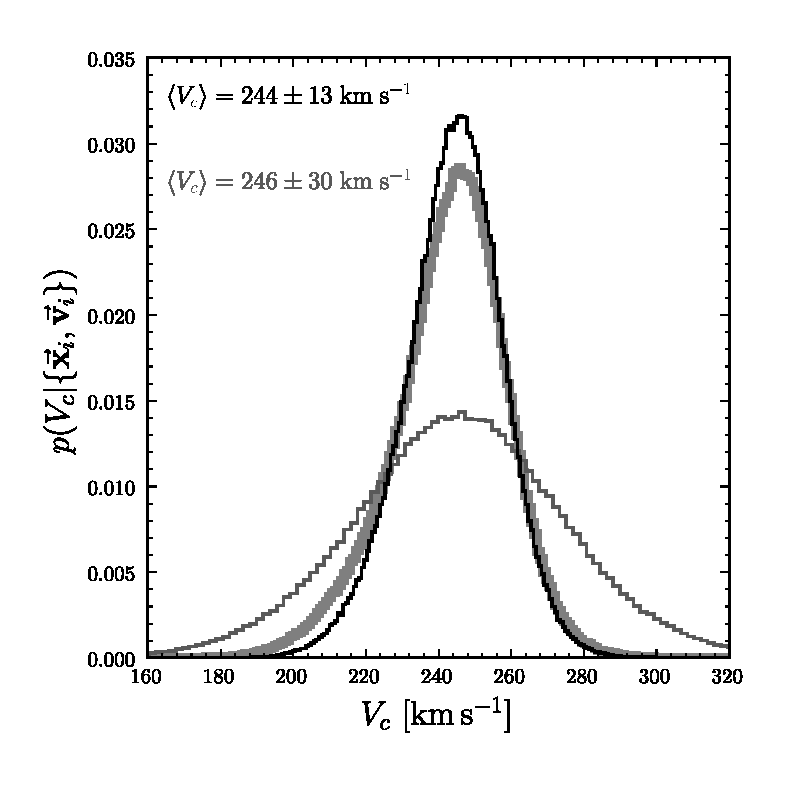
\includegraphics[width=.46\textwidth]{figs_masers/thetao_1M.eps}
\caption[Marginalized posterior probability distribution for the
  circular velocity]{Marginalized posterior probability distribution
  for the circular velocity $\vc$, shown as the black curve, and its
  mean (top label) from 10$^6$ MCMC samples. The prior probability
  distribution is shown as the thick gray curve; its mean is $\vc =
  243 \pm 16 $ km s$^{-1}$. The posterior and its mean (bottom label)
  obtained from dropping the informative prior on $\pmsgra$ is shown
  as the thin gray curve, illustrating that the maser data themselves
  constrain $\vc$ relatively weakly. The quoted uncertainty in mean
  value is the standard deviation $\equiv \sqrt{\langle \vc^2\rangle -
    \langle \vc\rangle^2}$.}\label{fig:thetao}
\end{figure}

\clearpage
\begin{figure}
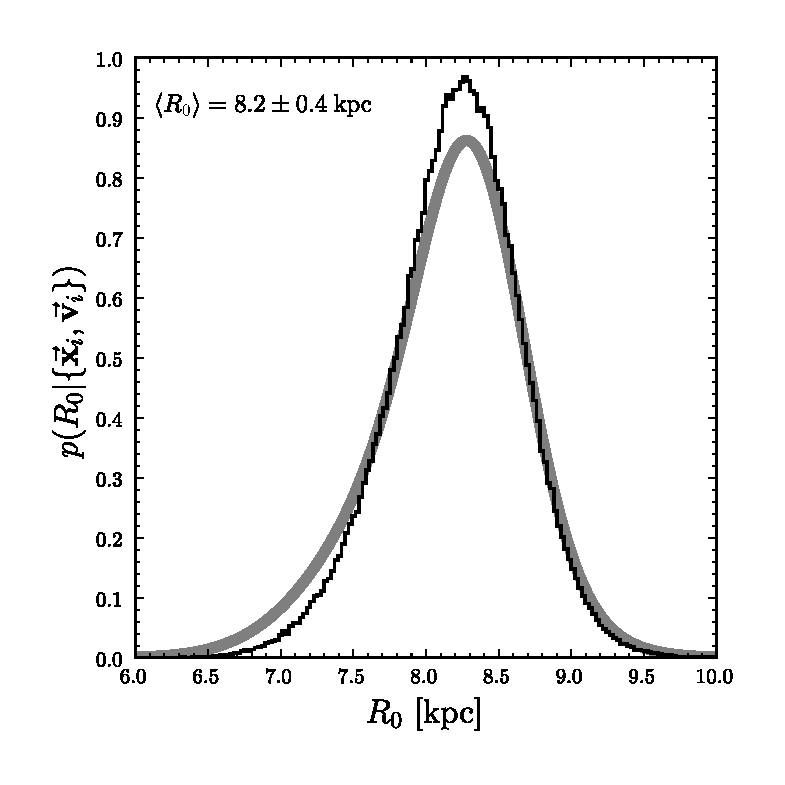
\includegraphics[width=.46\textwidth]{figs_masers/ro_1M.eps}
\caption[Marginalized posterior probability distribution for the
  distance to the Galactic center]{Marginalized posterior probability
  distribution for the distance \Ro\ to the Galactic center, shown as
  the black curve, from 10$^6$ MCMC samples. The prior probability
  distribution is shown as the thick gray curve; its mean is $R_0 =
  8.2 \pm 0.5$ kpc.}\label{fig:ro}
\end{figure}


\clearpage
\begin{figure}
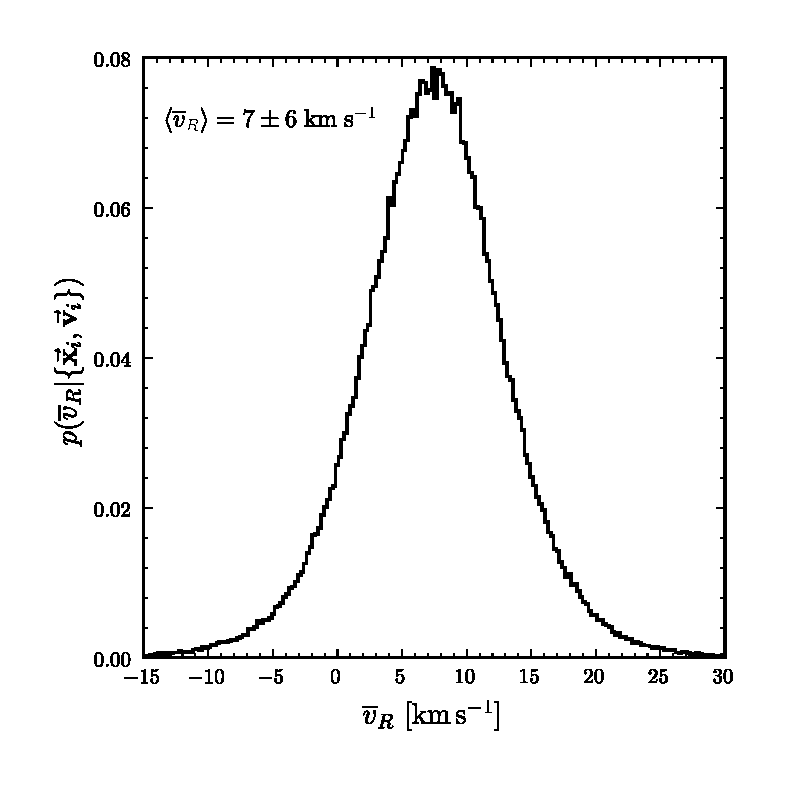
\includegraphics[width=.46\textwidth]{figs_masers/mean_1M_R.eps}
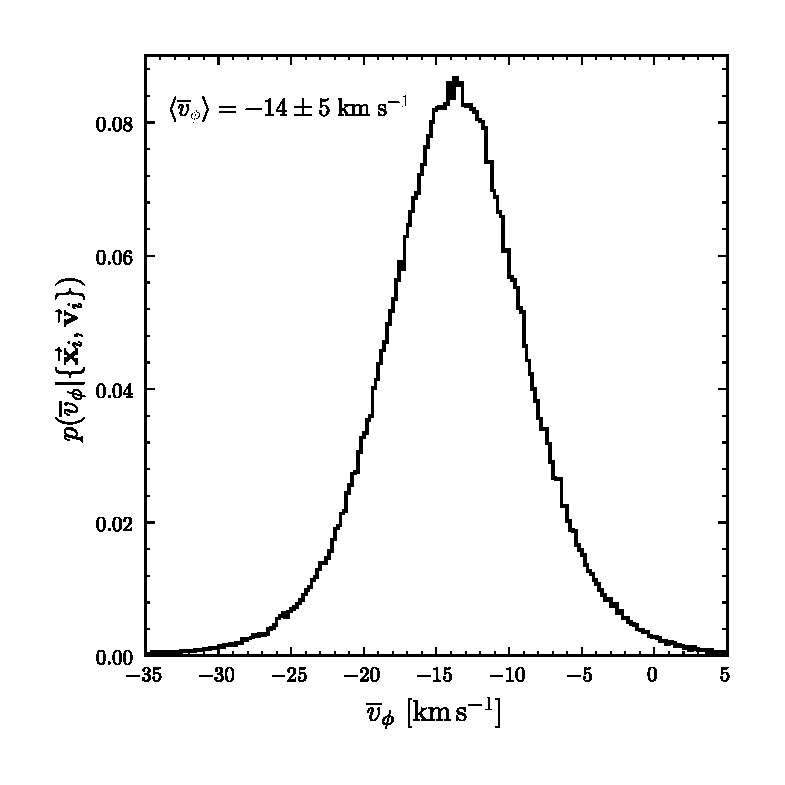
\includegraphics[width=.46\textwidth]{figs_masers/mean_1M_phi.eps}\\
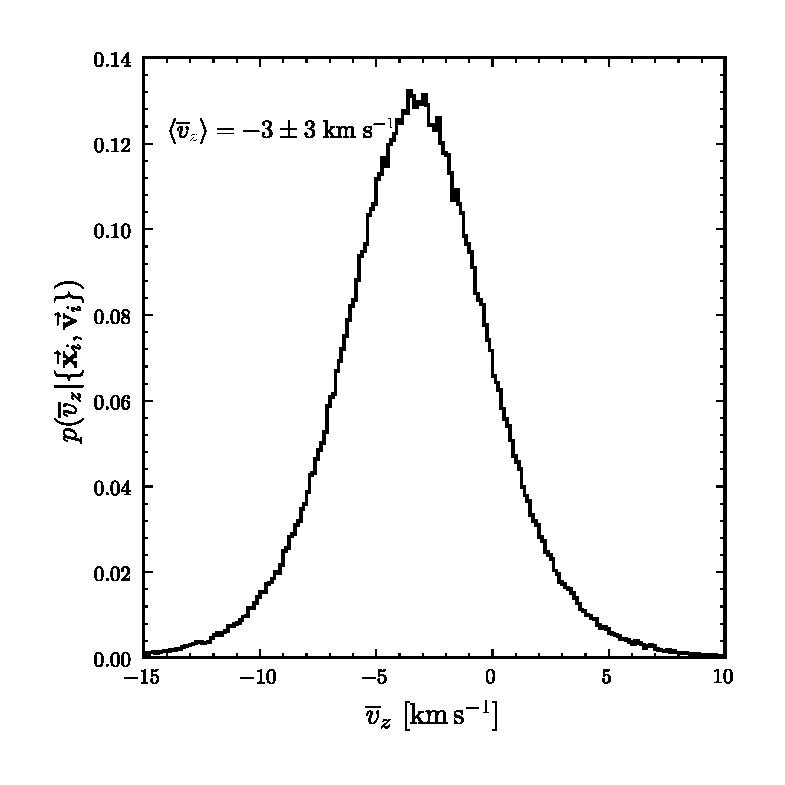
\includegraphics[width=.46\textwidth]{figs_masers/mean_1M_z.eps}
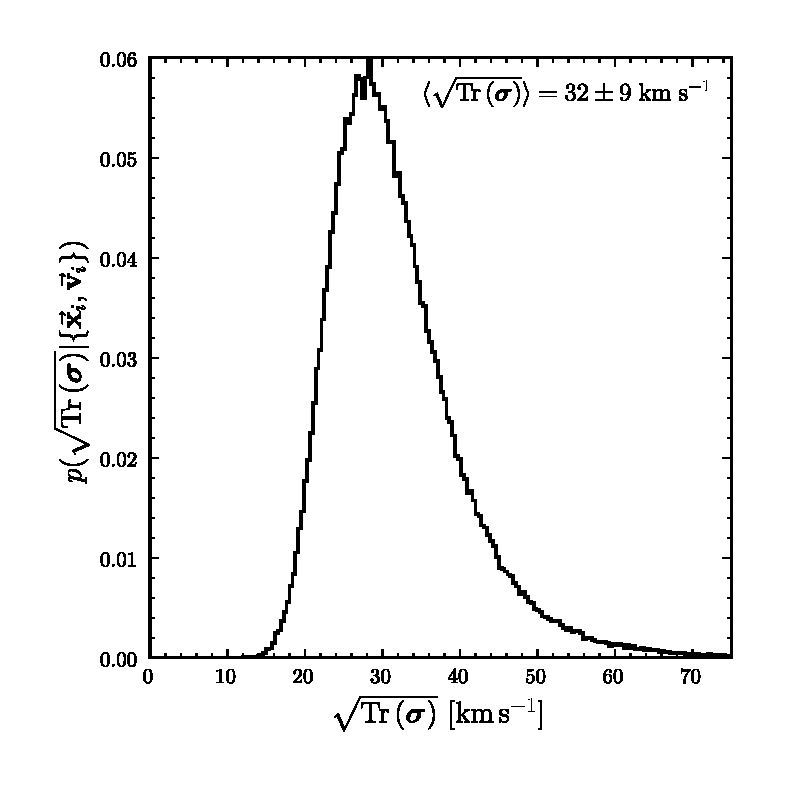
\includegraphics[width=.46\textwidth]{figs_masers/trV_1M.eps}
\caption[Marginalized posterior probability distribution for the
  parameters of the conditional velocity distribution of
  masers]{Marginalized posterior probability distribution for the
  parameters of the conditional velocity distribution of masers from
  10$^6$ samples: mean motion toward the Galactic Center (\emph{top
    left panel}); in the direction of Galactic rotation (\emph{top
    right panel}); toward the North Galactic Pole (\emph{bottom left
    panel}); the square root of the trace of the velocity dispersion
  tensor (\emph{bottom right panel}).}\label{fig:dist}
\end{figure}

\clearpage
\begin{figure}
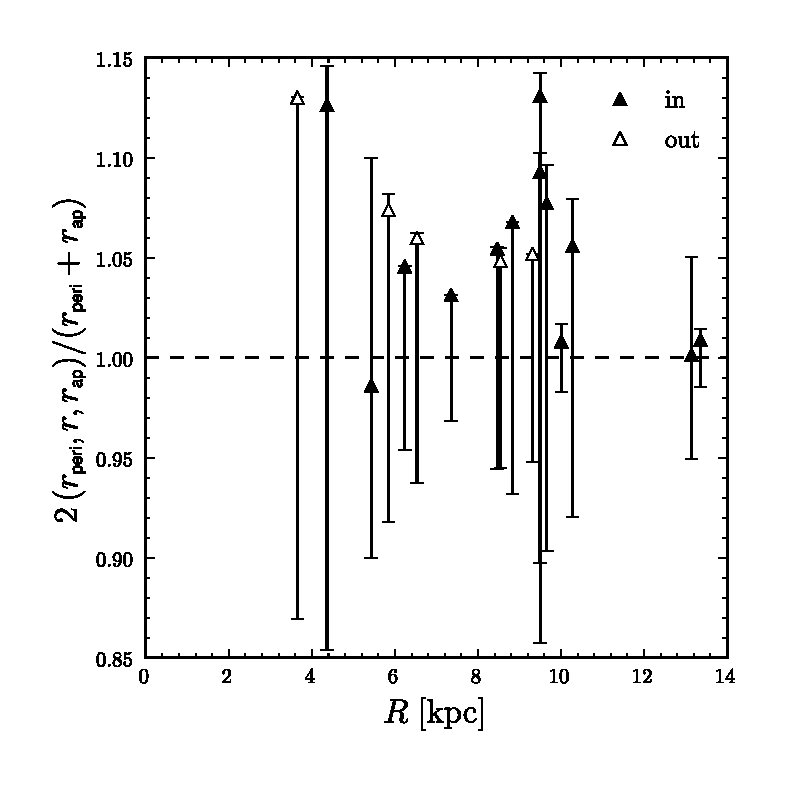
\includegraphics[width=.45\textwidth]{figs_masers/rrperirap.eps}
\caption[Orbital eccentricities and phases of the observed
  masers]{Orbital eccentricities and phases of the observed masers in
  a logarithmic potential: pericenter radius $r_{\mathrm{peri}}$,
  apocenter radius $r_{\mathrm{ap}}$, and current radius of the
  masers, normalized by the mean of the pericenter and apocenter
  radii, as a function of Galactocentric radius in a spherically
  symmetric logarithmic potential for $R_0 = 8.2$ kpc and $\vc = 244$
  km s$^{-1}$. Filled symbols indicate that the maser is moving toward
  the Galactic Center.}\label{fig:phases}
\end{figure}



%\input{chap2} % further chapters -- change file names to meaningful things...
%\input{chap3}
%\part{Second Part\label{part:two}}%
%\input{chap4}
%\input{chap5}
%\input{chap6}
%%%%% Appendices start %%%%%%%%%%%%%%%%
%% Comment out the following line if your thesis has no appendix
%\appendix
%\input{app1}
%% Note: If your thesis has more than one appendix, NYU requires a "list of
%% appendices" page before the body of the thesis. I don't provide the tools
%% to create that here, so you're on your own for that one... Sorry.
%\input{app2}
%%%% Input bibliography file %%%%%%%%%%%%%%%
\begin{thebibliography}{99}\addcontentsline{toc}{chapter}{Bibliography}

%%BOVY: MOVING GROUPS I
\expandafter\ifx\csname natexlab\endcsname\relax\def\natexlab#1{#1}\fi

\bibitem[Aarseth \& Woolf(1972)]{Aarseth72a}
  Aarseth,~S.~J. \& Woolf,~N.~J., 1972,
  \aplett, 12, 159

\bibitem[Adams \etal(2001)]{Adams01a}
  Adams,~J.~D., Stauffer,~J.~R., Monet,~D.~G., Skrutskie,~M.~F., \& Beichman,~C.~A., 2001,
  \aj, 121, 2053

\bibitem[Adelberger, Heckel, \& Nelson(2003)]{adelberger}
  Adelberger,~E.~G., Heckel,~B.~R., \& Nelson,~A.~E., 2003,
%  Tests of the Gravitational Inverse-Square Law,
%  \textit{Annu.~Rev.~Nucl.~Part.~Sci.}, 53, 77
  Annu.~Rev.~Nucl.~Part.~Sci., 53, 77

\bibitem[Afflerbach, Churchwell, \& Werner(1997)]{Afflerbach97a}
  Afflerbach,~A., Churchwell,~E., \& Werner,~W.~M., 1997,
  \apj, 478, 190

\bibitem[{{Akaike}(1974)}]{Akaike}
{Akaike}, H. 1974, {IEEE Transactions on Automatic Control}, 19, 716

\bibitem[Allison \etal(2009)]{Allison09a}
  Allison,~R.~J., Goodwin,~S.~P., Parker,~R.~J., de Grijs,~R., Portegies Zwart,~S.~F., \& Kouwenhoven,~M.~B.~N., 2009,
  \apjl, 700, L99

\bibitem[Anderson \& Darling(1952)]{AndersonDarling}
  Anderson,~T.~W. \& Darling,~D.~A., 1952,
%  Asymptotic theory of certain ``goodness-of-fit'' criteria based on stochastic processes, 
%  \textit{Annals\,Math.\,Stat.}, 23, 193
  Ann.\,Math.\,Stat., 23, 193

\bibitem[{{Antoja} {et~al.}(2008){Antoja}, {Figueras}, {Fern{\'a}ndez}, \&
  {Torra}}]{2008A&A...490..135A}
{Antoja}, T., {Figueras}, F., {Fern{\'a}ndez}, D., \& {Torra}, J. 2008, \aap,
  490, 135

\bibitem[Antoja \etal(2009)]{Antoja09a}
  Antoja,~T., Valenzuela,~O., Pichardo,~B., Moreno,~E., Figueras,~F., \& Fern{\'a}ndez,~D., 2009,
  \apjl, 700, L78

\bibitem[Ascenso, Alves, \& Lago(2009)]{Ascenso09a}
  Ascenso,~J., Alves,~J., \& Lago,~M.~T.~V.~T., 2009,
  \aap, 495, 147

\bibitem[Asiain, Figueras, \& Torra(1999)]{Asiain99a}
  Asiain,~R., Figueras,~F., \& Torra,~J., 1999,
  \aap, 350, 434

\bibitem[{{Asiain} {et~al.}(1999){Asiain}, {Figueras}, {Torra}, \&
  {Chen}}]{1999A&A...341..427A}
{Asiain}, R., {Figueras}, F., {Torra}, J., \& {Chen}, B. 1999, \aap, 341, 427

\bibitem[Aumer \& Binney(2009)]{Aumer09a}
  Aumer,~M.~\& Binney,~J.~J., 2009,
  \mnras, 397, 1286

\bibitem[{{Baade}(1944)}]{1944ApJ...100..137B}
{Baade}, W. 1944, \apj, 100, 137

\bibitem[{{Baade}(1958)}]{baade1958a}
{Baade}, W. 1958, in {Stellar Populations: Proceedings of the conference
  sponsored by the Pontifical Academy of Science and the Vatican Observatory,
  May 20-28, 1957}, ed. D.~J.~K. {O'Connell} ({Amsterdam}: {North-Holland
  Pub.~Co.}), 3

\bibitem[{{Bahcall} \& {Soneira}(1980)}]{1980ApJS...44...73B}
{Bahcall}, J.~N. \& {Soneira}, R.~M. 1980, \apjs, 44, 73

\bibitem[{{Bahcall} \& {Soneira}(1984)}]{1984ApJS...55...67B}
{Bahcall}, J.~N. \& {Soneira}, R.~M. 1984, \apjs, 55, 67

\bibitem[Bailer-Jones(2008)]{bailerjones08a}
  Bailer-Jones, ~C.~A.~L., 2008,
  in IAU Symp.~254, The Galaxy Disk in Cosmological Context, ed.~J.~Andersen, J.~Bland-Hawthorn, \& B.~Nordstr\"{o}m, (Dordrecht: Kluwer), 475  

\bibitem[Beloborodov \& Levin(2004)]{roulette}
  Beloborodov,~A.~M. \& Levin,~Y., 2004,
%  Orbital roulette:\ A new method of gravity estimation from observed motions,
%  \textit{Astrophys.\,J.}, 613, 224
  \apj, 613, 224
\bibitem[Beloborodov \etal(2006)]{Beloborodov06a} 
  Beloborodov,~A.~M, Levin,~Y., Eisenhauer,~F., Genzel,~R., 
  Paumard,~T., Gillessen,~S.,
  \& Ott,~T., 2004,
%  Clockwise stellar disk and the dark mass in the Galactic Center,
%  \textit{Astrophys.\,J.}, 648, 405
  \apj, 648, 405

\bibitem[Belokurov \etal(2006)]{belokurovfield}
  Belokurov,~V., \etal, 2006,
%  The Field of Streams: Sagittarius and its siblings,
%  \textit{Astrophys.\,J.\,Lett.}, 642, 137
  \apjl, 642, L137
\bibitem[Belokurov \etal(2007)]{belokurov}
  Belokurov,~V., \etal, 2007,
%  Cats and dogs, hair and a hero: A quintet of New Milky Way companions,
%  \textit{Astrophys.\,J.}, 654, 897
  \apj, 654, 897

\bibitem[Benjamin \etal(2005)]{Benjamin05a}
  Benjamin,~R.~A., \etal, 2005, \apj, 630, 149

\bibitem[Bensby \etal(2007)]{Bensby07a}
  Bensby,~T., Oey,~M.~S., Feltzing,~S., \& Gustafsson,~B., 2007,
  \apjl, 655, L89

\bibitem[Bertelli \etal(1994)]{Bertelli94a}
  Bertelli,~G., Bressan,~A., Chiosi,~C., Fagotto,~F., \& Nasi, E., 1994,
  \aaps, 106, 275

\bibitem[{{Bienaym{\'e}}(1999)}]{1999A&A...341...86B}
{Bienaym{\'e}}, O. 1999, \aap, 341, 86

\bibitem[Binney, Gerhard, \& Spergel(1997)]{binney97a}
  Binney,~J.~J., Gerhard,~O., \& Spergel,~D.~N., 1997,
  \mnras, 288, 365

\bibitem[{{Binney} \& {Merrifield}(1998)}]{1998gaas.book.....B}
{Binney}, J. \& {Merrifield}, M. 1998, {Galactic Astronomy} (Princeton
  University Press)

\bibitem[{{Binney} {et~al.}(1997){Binney}, {Dehnen}, {Houk}, {Murray}, \&
  {Penston}}]{1997ESASP.402..473B}
{Binney}, J.~J., {Dehnen}, W., {Houk}, N., {Murray}, C.~A., \& {Penston}, M.~J.
  1997, in ESA Special Publication, Vol. 402, Hipparcos - Venice '97, 473

\bibitem[{{Binney} \& {Tremaine}(2008)}]{2008gady.book.....B}
{Binney}, J. \& {Tremaine}, S. 2008, {Galactic Dynamics: Second Edition}
  (Princeton University Press)

\bibitem[Bissantz \& Gerhard(2002)]{bissantz02a}
  Bissantz,~N.~\& Gerhard,~O., 2002,
  \mnras, 330, 591

\bibitem[{{Blaauw} {et~al.}(1960){Blaauw}, {Gum}, {Pawsey}, \&
  {Westerhout}}]{1960MNRAS.121..123B}
{Blaauw}, A., {Gum}, C.~S., {Pawsey}, J.~L., \& {Westerhout}, G. 1960, \mnras,
  121, 123

\bibitem[Blaauw(1970)]{Blaauw70a}
  Blaauw,~A., 1970, in The Spiral Structure of our Galaxy, Proceedings from 38th IAU Symposium, Vol.~38, ed.~W.~Becker \& I.~Kontopoulos, 199

\bibitem[Blitz \& Spergel(1991)]{Blitz91a}
  Blitz,~L.~\& Spergel,~D.~N., 1991, \apj, 379, 631

\bibitem[{{Boesgaard} \& {Budge}(1988)}]{1988ApJ...332..410B}
{Boesgaard}, A.~M. \& {Budge}, K.~G. 1988, \apj, 332, 410

\bibitem[Boesgaard \& Friel(1990)]{Boesgaard90a}
  Boesgaard,~A.~M. \& Friel,~E.~D., 1990,
  \apj, 351, 467

\bibitem[Bok(1934)]{Bok34a}
  Bok,~B.~J., 1934,
  Harvard Circ., 384, 1

\bibitem[Bok(1936)]{Bok36a}
  Bok,~B.~J., 1936,
  Observatory, 59, 76

\bibitem[Bok(1946)]{Bok46a}
  Bok,~B.~J., 1946,
  \mnras, 106, 61

\bibitem[{{Boss}(1911)}]{1911AJ.....27...33B}
{Boss}, B. 1911, \aj, 27, 33

\bibitem[{{Boss}(1908)}]{boss08a}
{Boss}, L. 1908, \aj, 26, 31

\bibitem[Bonnell \& Davies(1998)]{Bonnell98a}
  Bonnell,~I.~A. \& Davies,~M.~B., 1998,
  \mnras, 295, 691

\bibitem[Bouvier \etal(1998)]{Bouvier98a}
  Bouvier,~J., Stauffer,~J.~R., Martin,~E.~L., Barrado y Navascues,~D., Wallace,~B., \& Bejar,~V.~J.~S., 1998,
  \aap, 336, 490

\bibitem[Bouvier \etal(2008)]{Bouvier08a}
  Bouvier,~J., \etal, 2008,
  \aap, 481, 661

\bibitem[Bovy \& Hogg(2010)]{Bovy10a} Bovy,~J.~\& Hogg,~D.~W., 2010,
  \apj, 717, 617

%\bibitem[Bovy, Murray, \& Hogg(2010)]{Bovy10b} Bovy,~J., Murray, I., \& Hogg,~D.~W., 2010,
%  \apj, 711, 1157

\bibitem[Bovy \etal(2009a)]{Bovy09b}
  Bovy,~J., Hogg,~D.~W., \& Rix, H.-W., 2009a,
  \apj, 704, 1704

\bibitem[Bovy \etal(2009b)]{Bovyveldist}
  Bovy,~J., Hogg,~D.~W., \& Roweis,~S.~T., 2009b,
%  The velocity distribution of nearby stars from \emph{Hipparcos} data. I. The significance of the moving groups,
%  \textit{Astrophys.\,J.}, 700, 1794
  \apj, 700, 1794 (\bhr)

\bibitem[{{Bovy} {et~al.}(2009c){Bovy}, {Hogg}, \& {Roweis}}]{BovyXD}
{Bovy}, J., {Hogg}, D.~W., \& {Roweis}, S.~T. 2009c, {arXiv:0905.2979 [stat.ME]}

\bibitem[{{Boyle} \& {McClure}(1975)}]{1975PASP...87...17B}
{Boyle}, R.~J. \& {McClure}, R.~D. 1975, \pasp, 87, 17

\bibitem[{{Bozdogan}(1983)}]{Bozdogan}
{Bozdogan}, H. 1983, {Determining the number of component clusters in the
  standard multivariate normal mixture model using model-selection criteria},
  Tech. rep., {TR UIC/DQM/A83-1, Quantitative Methods Dept., University of
  Illinois}

\bibitem[{{Breger}(1968)}]{1968PASP...80..578B}
{Breger}, M. 1968, \pasp, 80, 578

\bibitem[{{Cabrera-Ca\~{n}o} \& {Alfaro}(1990)}]{1990A&A...235...94C}
{Cabrera-Ca\~{n}o}, J. \& {Alfaro}, E.~J. 1990, \aap, 235, 94

\bibitem[Caloi \etal(1999)]{Caloi99a}
  Caloi,~V., Cardini,~D., D'Antona,~F., Badiali,~M., Emanuele,~A., \& Mazzitelli,~I., 1999,
  \aap, 351, 925

\bibitem[Carlberg \& Sellwood(1985)]{Carlberg85a}
  Carlberg,~R.~G.~\& Sellwood,~J.~A., 1985,
  \apj, 292, 79

\bibitem[Carraro \etal(2007)]{Carraro07a}
  Carraro,~G., de La Fuente Marcos,~R., Villanova,~S., Moni Bidin,~C., de La Fuente Marcos,~C., Baumgardt,~H., \& Solivella,~G., 2007,
  %title = ``{Observational templates of star cluster disruption. The stellar group NGC 1901 in front of the Large Magellanic Cloud}'',
  \aap, 466, 931

\bibitem[Chakrabarty(2007)]{Chakrabarty07a}
  Chakrabarty,~D., 2007,
  \aap, 467, 145

\bibitem[{{Chaudhuri}(1940)}]{1940MNRAS.100..574C}
{Chaudhuri}, P.~C. 1940, \mnras, 100, 574

\bibitem[{{Chen} {et~al.}(1997){Chen}, {Asiain}, {Figueras}, \&
  {Torra}}]{1997A&A...318...29C}
{Chen}, B., {Asiain}, R., {Figueras}, F., \& {Torra}, J. 1997, \aap, 318, 29

\bibitem[{{Chereul} {et~al.}(1998){Chereul}, {Creze}, \&
  {Bienayme}}]{1998A&A...340..384C}
{Chereul}, E., {Creze}, M., \& {Bienayme}, O. 1998, \aap, 340, 384

\bibitem[{{Chereul} {et~al.}(1999){Chereul}, {Cr{\'e}z{\'e}}, \&
  {Bienaym{\'e}}}]{1999A&AS..135....5C}
{Chereul}, E., {Cr{\'e}z{\'e}}, M., \& {Bienaym{\'e}}, O. 1999, \aaps, 135, 5

\bibitem[Chereul \& Grenon(2001)]{Chereul01a}
  Chereul,~E. \& Grenon,~M., 2001, in Dynamics of Star Clusters and the
  Milky Way, ASP Conference Series, Vol. 228, ed.~S.~Deiters, B.~Fuchs,
  A.~Just, R.~Spurzem, \& R.~Wielen (San Francisco, CA: ASP), 398

\bibitem[Cole \& Weinberg(2002)]{cole02a}
  Cole,~A.~A.~\& Weinberg,~M.~D., 2002,
  \apjl, 574, L43

\bibitem[Contopoulos(1975)]{Contopoulos75a}
  Contopoulos,~G., 1975,
  \apj, 201, 566

\bibitem[Contopoulos \& Grosb\o l(1986)]{Contopoulos86a}
  Contopoulos,~G.~\& Grosb\o l,~P., 1986,
  \aap, 155, 11

\bibitem[Contopoulos \& Grosb\o l(1989)]{Contopoulos89a}
  Contopoulos,~G.~\& Grosb\o l,~P., 1989,
  A\&AR, 1, 261

\bibitem[{{Conway} \& {Sloane}(1992)}]{conway92a}
{Conway}, J.~H. \& {Sloane}, N. J.~A. 1992, {Sphere Packings, Lattices and
  Groups} (London: {Springer-Verlag})

\bibitem[{{Dehnen}(1998)}]{1998AJ....115.2384D}
{Dehnen}, W. 1998, \aj, 115, 2384

\bibitem[{{Dehnen} \& {Binney}(1998)}]{1998MNRAS.298..387D}
{Dehnen}, W. \& {Binney}, J.~J. 1998, \mnras, 298, 387

\bibitem[Dehnen(1999a)]{dehnen99b}
  Dehnen,~W., 1999a, \aj, 118, 1201

\bibitem[Dehnen(1999b)]{dehnen99c}
  Dehnen,~W., 1999b, \apj, 524, L35

\bibitem[Dehnen(2000)]{dehnen00a}
  Dehnen,~W., 2000, \aj, 119, 800

\bibitem[de la Fuente Marcos(1995)]{delafuentemarcos95a}
  de la Fuente Marcos,~R., 1995,
  \aap, 301, 407

\bibitem[{{Dempster} {et~al.}(1977){Dempster}, {Laird}, \&
  {Rubin}}]{Dempster1977}
{Dempster}, A.~P., {Laird}, N.~M., \& {Rubin}, D.~B. 1977, Journal of the Royal
  Statistical Society. Series B (Methodological), 39, 1

\bibitem[De Silva \etal(2007)]{DeSilva07a}
  De Silva,~G.~M., Freeman,~K.~C., Bland-Hawthorn,~J., Asplund,~M., \& Bessell,~M.~S., 2007,
  \aj, 133, 694

\bibitem[De Simone, Wu, \& Tremaine(2004)]{deSimone04a}
  De Simone,~R., Wu,~X., \& Tremaine,~S., 2004,
  \mnras, 350, 627

\bibitem[de Zeeuw \etal(1999)]{deZeeuw99a}
  de Zeeuw,~P.~T., Hoogerwerf,~R., de Bruijne,~J.~H.~J., Brown,~A.~G.~A., \& Blaauw,~A., 1999,
  \aj, 117, 354

\bibitem[Dobbie \etal(2002)]{Dobbie02a}
  Dobbie,~P.~D., Kenyon,~F., Jameson,~R.~F., Hodgkin,~S.~T., Hambly,~N.~C., \& Hawkins,~M.~R.~S., 2002,
  \mnras, 329, 543

\bibitem[{{Eddington}(1910)}]{1910MNRAS..71...43E}
{Eddington}, A.~S. 1910, \mnras, 71, 43

\bibitem[Eggen(1958)]{Eggen58a}
  Eggen,~O.~J., 1958,
  \mnras, 118, 65

\bibitem[{{Eggen}(1958)}]{1958MNRAS.118..154E}
{Eggen}, O.~J. 1958, \mnras, 118, 154

\bibitem[{{Eggen}(1959{\natexlab{a}})}]{1959Obs....79..182E}
{Eggen}, O.~J. 1959{\natexlab{a}}, The Observatory, 79, 182

\bibitem[{{Eggen}(1959{\natexlab{b}})}]{1959Obs....79...88E}
{Eggen}, O.~J. 1959{\natexlab{b}}, The Observatory, 79, 88

\bibitem[{{Eggen}(1964)}]{1964RGOB...84..111E}
{Eggen}, O.~J. 1964, Roy.~Greenwich Obs.~Bull., 84, 111

\bibitem[{{Eggen}(1965)}]{1965Obs....85..191E}
{Eggen}, O.~J. 1965, The Observatory, 85, 191

\bibitem[{{Eggen}(1969)}]{1969PASP...81..553E}
{Eggen}, O.~J. 1969, \pasp, 81, 553

\bibitem[{{Eggen}(1970)}]{1970PASP...82...99E}
{Eggen}, O.~J. 1970, \pasp, 82, 99

\bibitem[{{Eggen}(1971{\natexlab{a}})}]{1971PASP...83..271E}
{Eggen}, O.~J. 1971{\natexlab{a}}, \pasp, 83, 271

\bibitem[{{Eggen}(1971{\natexlab{b}})}]{1971PASP...83..251E}
{Eggen}, O.~J. 1971{\natexlab{b}}, \pasp, 83, 251

\bibitem[{{Eggen}(1978)}]{1978ApJ...222..203E}
{Eggen}, O.~J. 1978, \apj, 222, 203

\bibitem[{{Eggen}(1983)}]{1983AJ.....88..813E}
{Eggen}, O.~J. 1983, \aj, 88, 813

\bibitem[{{Eggen}(1986)}]{1986AJ.....92..910E}
{Eggen}, O.~J. 1986, \aj, 92, 910

\bibitem[Eggen(1993)]{Eggen93a}
  Eggen,~O.~J., 1993,
  \aj, 106, 1885

\bibitem[Eggen(1996)]{Eggen96a}
  Eggen,~O.~J., 1996,
  \aj, 112, 1595

\bibitem[{{Eggen} \& {Sandage}(1959)}]{1959MNRAS.119..255E}
{Eggen}, O.~J. \& {Sandage}, A.~R. 1959, \mnras, 119, 255

\bibitem[Eisenstein \etal(2005)]{Eisenstein05a}
  Eisenstein,~D.~J., \etal, 2005, \apj, 633, 560

\bibitem[Elmegreen \& Elmegreen(1982)]{Elmegreen82a}
  Elmegreen,~D.~M.~\& Elmegreen,~B.~G., 1983,
  \mnras, 201, 1021

\bibitem[Elmegreen \& Elmegreen(1983)]{Elmegreen83a}
  Elmegreen,~D.~M.~\& Elmegreen,~B.~G., 1983,
  \apj, 267, 31

\bibitem[{{ESA}(1997)}]{ESA97a}
{ESA}, 1997, {The \emph{Hipparcos} and \emph{Tycho} Catalogues} (ESA SP-1200; Noordwijk: ESA)

\bibitem[{{Famaey} {et~al.}(2005){Famaey}, {Jorissen}, {Luri}, {Mayor}, {Udry},
    {Dejonghe}, \& {Turon}}]{2005A&A...430..165F}
  {Famaey}, B., {Jorissen}, A., {Luri}, X., {Mayor}, M., {Udry}, S., {Dejonghe},
  H., \& {Turon}, C. 2005, \aap, 430, 165

\bibitem[Famaey \etal(2007)]{Famaey07a}
  Famaey,~B., Pont,~F., Luri,~X., Udry,~S., Mayor,~M., \& Jorissen,~A., 2007,
  \aap, 461, 957

\bibitem[Famaey, Siebert, \& Jorissen(2008)]{Famaey08a}
  Famaey,~B., Siebert,~A., \& Jorissen,~A., 2008,
  \aap, 483, 453

\bibitem[Feast \& Whitelock(1997)]{Feast97a} Feast,~M. \& Whitelock,~P., 1997,
  \mnras, 291, 683

\bibitem[Feltzing \& Holmberg(2000)]{Feltzing00a}
  Feltzing,~S.~\& Holmberg,~J., 2000,
  \aap, 357, 153
  
\bibitem[{{Figueras} {et~al.}(1997){Figueras}, {Gomez}, {Asiain}, {Chen},
  {Comeron}, {Grenier}, {Lebreton}, {Moreno}, {Sabas}, \&
  {Torra}}]{1997ESASP.402..519F}
{Figueras}, F., {Gomez}, A.~E., {Asiain}, R., {Chen}, B., {Comeron}, F.,
  {Grenier}, S., {Lebreton}, Y., {Moreno}, M., {Sabas}, V., \& {Torra}, J.
  1997, in ESA Special Publication, Vol. 402, Hipparcos - Venice '97, 519--524

\bibitem[Fischbach \& Talmadge(1999)]{fischbach}
  Fischbach,~E. \& Talmadge,~C.~L., 1999
  The Search for Non-Newtonian Gravity,
  (Springer-Verlag)

\bibitem[Flynn \etal(2006)]{Flynn06a}
  Flynn,~C., Holmberg,~J., Portinari,~L., Fuchs,~B., \& Jahrei{\ss},~H., 2006,
  \mnras, 372, 1149

\bibitem[{{Francis} \& {Anderson}(2009)}]{2009arXiv0901.3503F}
{Francis}, C. \& {Anderson}, E. 2009, arXiv:0901.3503 [astro-ph]

\bibitem[Freeman(1987)]{Freeman87a}
  Freeman,~K.~C., 1987, \araa, 25, 603

\bibitem[Freeman \& Bland-Hawthorn(2002)]{Freeman02a}
  Freeman,~K.~\& Bland-Hawthorn,~J., 2002,
  \araa, 40, 487

\bibitem[Freeman \etal(2010)]{Freeman10a}
  Freeman,~K., Bland-Hawthorn,~J., \& Barden,~S., 2010, 
  AAO Newsletter, 117, 9

\bibitem[Fux(2001)]{fux01a}
  Fux,~R., 2001,
  \aap, 373, 511

\bibitem[Gardner \& Flynn(2010)]{gardner10a}
  Gardner,~E.~\& Flynn,~C., 2010,
  \mnras, 405, 545

\bibitem[{{Gelman} {et~al.}(2000){Gelman}, {Carlin}, {Stern}, \&
  {Rubin}}]{Gelman00a}
{Gelman}, A., {Carlin}, J.~B., {Stern}, H.~S., \& {Rubin}, D.~B. 2000,
  {Bayesian Data Analysis} ({Chapman \& Hall/CRC})

\bibitem[Georgelin \& Georgelin(1976)]{Georgelin76a}
  Georgelin,~Y.~M. \& Georgelin,~Y.~P., 1976, \aap, 49, 57

\bibitem[{{Gerbaldi} {et~al.}(1989)}]{1989Msngr..56...12G}
{Gerbaldi}, M. {et~al.} 1989, ESO Messenger, 56, 12

\bibitem[Ghez \etal(2008)]{Ghez08a}
  Ghez,~A.~M., \etal, 2008,
  \apj, 689, 1044

\bibitem[{{Ghigna} {et~al.}(1998){Ghigna}, {Moore}, {Governato}, {Lake},
  {Quinn}, \& {Stadel}}]{ghigna98a}
{Ghigna}, S., {Moore}, B., {Governato}, F., {Lake}, G., {Quinn}, T., \&
  {Stadel}, J. 1998, \mnras, 300, 146

\bibitem[Gillessen \etal(2009)]{Gillessen09a}
  Gillessen,~S., Eisenhauer,~F., Trippe,~S., Alexander,~T., Genzel,~R., Martins,~F., \& Ott, T., 2009
  \apj, 692, 1075

\bibitem[{{Gilmore} \& {Reid}(1983)}]{1983MNRAS.202.1025G}
{Gilmore}, G. \& {Reid}, N. 1983, \mnras, 202, 1025

\bibitem[Giorgini \etal(1996)]{Giorgini96a}
  Giorgini,~J.~D., Yeomans,~D.~K., Chamberlin,~A.~B., Chodas,~P.~W., Jacobson,~R.~A., Keesey,~M.~S., Lieske,~J.~H., Ostro,~S.~J., Standish,~E.~M., \& Wimberly,~R.~N., 1996, 
%  JPL's On-Line Solar System Data Service,
%  \textit{Bull.\,Amer.\,Astron.\,Soc.}, 28, 1158
  \baas, 28, 1158

\bibitem[{{Gomez} {et~al.}(1990){Gomez}, {Delhaye}, {Grenier}, {Jaschek},
  {Arenou}, \& {Jaschek}}]{1990A&A...236...95G}
{Gomez}, A.~E., {Delhaye}, J., {Grenier}, S., {Jaschek}, C., {Arenou}, F., \&
  {Jaschek}, M. 1990, \aap, 236, 95

\bibitem[Gratton(2000)]{Gratton00a}
  Gratton,~R., 2000,
  in Stellar Clusters and Associations: Convection, Rotation, and Dynamos,
  ed.~R.~Pallavicini, G.~Micela, \& S.~Sciortino (San Francisco, CA: ASP),
  198, 225


\bibitem[{{Green}(1985)}]{Green85a}
{Green}, R.~M. 1985, {Spherical astronomy} (Cambridge University Press)

\bibitem[{{Grenier} {et~al.}(1985){Grenier}, {Gomez}, {Jaschek}, {Jaschek}, \&
  {Heck}}]{1985A&A...145..331G}
{Grenier}, S., {Gomez}, A.~E., {Jaschek}, C., {Jaschek}, M., \& {Heck}, A.
  1985, \aap, 145, 331

\bibitem[{{Gr{\"u}nwald}(2007)}]{Grunwaldbook}
{Gr{\"u}nwald}, P.~D. 2007, {The minimum description length principle}
  (Cambridge, Massachusetts: {MIT Press})

\bibitem[Hambly \etal(1999)]{Hambly99a}
  Hambly,~N.~C., Hodgkin,~S.~T., Cossburn,~M.~R., \& Jameson,~R.~F., 1999,
  \mnras, 303, 835

\bibitem[{{Helmi} {et~al.}(2003){Helmi}, {White}, \&
  {Springel}}]{2003MNRAS.339..834H}
{Helmi}, A., {White}, S.~D.~M., \& {Springel}, V. 2003, \mnras, 339, 834

\bibitem[{{Hertzsprung}(1909)}]{1909ApJ....30..135H}
{Hertzsprung}, E. 1909, \apj, 30, 135

\bibitem[Hillenbrand \& Hartmann(1998)]{Hillenbrand98a}
  Hillenbrand,~L.~A. \& Hartmann,~L.~W., 1998,
  \apj, 492, 540

\bibitem[H{\o}g \etal(2000a)]{hog00a}
  H{\o}g,~E., Fabricius,~C., Makarov,~V.~V., Urban,~S., Corbin,~T., Wycoff,~G., Bastian,~U., Schwekendiek,~P., \& Wicenec,~A., 2000a,
  \aap, 355, L27

\bibitem[H{\o}g \etal(2000b)]{hog00b}
  H{\o}g,~E., Fabricius,~C., Makarov,~V.~V., Bastian,~U., Schwekendiek,~P., Wicenec,~A., Urban,~S., Corbin,~T., \& Wycoff,~G., 2000b
    \aap, 357, 367

\bibitem[{{Hogg} {et~al.}(2005){Hogg}, {Blanton}, {Roweis}, \&
  {Johnston}}]{2005ApJ...629..268H}
{Hogg}, D.~W., {Blanton}, M.~R., {Roweis}, S.~T., \& {Johnston}, K.~V. 2005,
  \apj, 629, 268

\bibitem[Holmberg, Nordstr{\"o}m, \& Andersen(2007)]{Holmberg07a}
  Holmberg,~J., Nordstr\"{o}m,~B., \& Andersen,~J., 2007,
  \aap, 475, 519

\bibitem[Holmberg, Nordstr{\"o}m, \& Andersen(2009)]{Holmberg09a}
  Holmberg,~J., Nordstr\"{o}m,~B., \& Andersen,~J., 2009,
  \aap, 501, 941

\bibitem[{{Ivezi{\'c}} {et~al.}(2008)}]{2008ApJ...684..287I}
{Ivezi{\'c}}, {\v Z}. {et~al.} 2008, \apj, 684, 287

\bibitem[Jaynes(2003)]{jaynes}
  Jaynes,~E.~T., 2003,
  \textit{Probability theory: the logic of science} (Cambridge University Press)

\bibitem[Jeans(1915)]{Jeans15a}
  Jeans,~J.~H., 1915,
  \mnras, 76, 70

\bibitem[Jeans(1935)]{Jeans35a}
  Jeans,~J.~H., 1935,
  Observatory, 58, 108

\bibitem[Jeffreys(1939)]{Jeffreys39a}
  Jeffreys,~H., 1939,
  %\textit{Theory of Probability} (Oxford: Clarendon Press)
  Theory of Probability (Oxford: Clarendon Press)

\bibitem[{{Johnson} \& {Soderblom}(1987)}]{1987AJ.....93..864J}
{Johnson}, D.~R.~H. \& {Soderblom}, D.~R. 1987, \aj, 93, 864

\bibitem[{{Johnston}(1998)}]{johnston98a}
{Johnston}, K.~V. 1998, \apj, 495, 297

\bibitem[Johnston \etal(1999)]{Johnston99}
  Johnston,~K.~V., Zhao,~H., Spergel,~D.~N., \& Hernquist, L., 1999,
%  Tidal streams as probes of the Galactic potential,
%  \textit{Astrophys.\,J.\,Lett.}, 512, L109 
  \apjl, 512, L109 

\bibitem[de Jong \etal(2010)]{deJong10a}
  de Jong,~J.~T.~A., Yanny,~B., Rix,~H.-W., Dolphin,~A.~E., Martin,~N.~F., \& Beers,~T.~C., 2010, \apj, 714, 663

\bibitem[Juri\'{c} \etal(2008)]{Juric08a}
  Juri\'{c},~M., \etal, 2008, \apj, 673, 864

\bibitem[Kaasalainen \& Binney(1994)]{Binney94}
  Kaasalainen,~M. \& Binney,~J., 1994,
%  Construction of invariant tori and integrable Hamiltonians,
%  \textit{Phys.\,Rev.\,Lett.}, 73, 2377
  Phys.\,Rev.\,Lett., 73, 2377

\bibitem[Kalnajs(1991)]{Kalnajs91a}
  Kalnajs,~A., 1991, in Dynamics of Disc Galaxies, ed.~B.~Sundelius (G\"{o}teborg: Dept. Astron. Astrophys., G\"{o}teborg Univ.), 323

\bibitem[{{Kapteyn}(1905)}]{kapteyn05a}
{Kapteyn}, J.~C. 1905, {British Assoc.~Adv.~Sci.~Rep.}, Sec.~A, 257

\bibitem[{{Kapteyn}(1914)}]{1914ApJ....40...43K}
{Kapteyn}, J.~C. 1914, \apj, 40, 43

\bibitem[Katz \etal(2004)]{Katz04a}
  Katz,~D., \etal, 2004,
\mnras, 354, 1223

\bibitem[Kendall(1938)]{Kendall38a}
  Kendall,~M., 1938,
%  A new measure of rank correlation,
%  \textit{Biometrika}, 30, 81
  Biometrika, 30, 81

\bibitem[Kepler(1609)]{Kepler}
  Kepler,~J., 1609,
%  \textit{Astronomia Nova},
  Astronomia Nova,
  trans.\ W.~H.~Donahue, 1992
  (Cambridge University Press)

\bibitem[King \etal(2003)]{King03a}
  King,~J.~R., Villarreal,~A.~R., Soderblom,~D.~R., Gulliver,~A.~F., \& Adelman,~S.~J., 2003,
  %title = ``{Stellar Kinematic Groups. II. A Reexamination of the Membership, Activity, and Age of the Ursa Major Group}'',
  \aj, 125, 1980

\bibitem[Klypin, Zhao, \& Sommerville(2002)]{Klypin02a}
  Klypin,~A., Zhao,~H., \& Somerville,~R.~S., 2002,
  \apj, 573, 597

\bibitem[Klypin \etal(1999)]{Klypin99a}
  Klypin,~A., Kravtsov,~A.~V., Valenzuela,~O., \& Prada,~F., 1999, \apj, 522, 82

\bibitem[Kochanek(1996)]{Kochanek96a}
  Kochanek,~C.~S., 1996,
  \apj, 457, 228

\bibitem[Kolmogorov(1941)]{Kolmogorov41a}
  Kolmogorov,~A.~N., 1941,
%  Confidence limits for an unknown distribution function,
%  \textit{Ann.~Math.~Stat.}, 12, 461
  Ann.~Math.~Stat., 12, 461

\bibitem[{{Kolmogorov}(1965)}]{kolmogorov65a}
{Kolmogorov}, A.~N. 1965, {Problems.~Inform.~Transmission}, 1, 1

\bibitem[Komatsu \etal(2011)]{Komatsu11a}
  Komatsu,~E., \etal, 2011, \apjs, 192, 18

\bibitem[{{Koposov} {et~al.}(2008)}]{koposov}
{Koposov}, S.~E. {et~al.} 2008, \apj, 686, 279

\bibitem[{{Koposov} {et~al.}(2009){Koposov}, {Yoo}, {Rix}, {Weinberg},
  {Macci{\`o}}, \& {Escud{\'e}}}]{Koposov:2009ru}
{Koposov}, S.~E., {Yoo}, J., {Rix}, H.-W., {Weinberg}, D.~H., {Macci{\`o}},
  A.~V., \& {Escud{\'e}}, J.~M. 2009, \apj, 696, 2179

\bibitem[Koposov, Rix, \& Hogg(2009)]{Koposov09a} Koposov,~S.~E., Rix,~H.-W., \& Hogg,~D.~W., 2009, arXiv:0907.1085 [astro-ph]

\bibitem[Kuijken \& Gilmore(1989)]{Kuijken89a}
  Kuijken,~K.~\& Gilmore,~G., 1989, \mnras, 239, 605

\bibitem[Kuiper(1962)]{Kuiper62a}
  Kuiper,~N.~H., 1962,
%  Tests concerning random points on a circle,
%  \textit{Proc.~Koninklijke Nederlandse Akademie van Wetenschappen A}, 63, 38
  Proc.~Koninklijke Nederlandse Akademie van Wetenschappen A, 63, 38

\bibitem[Leonard \& Tremaine(1990)]{Leonard90a}
  Leonard,~P.~J.~T. \& Tremaine,~S., 1990,
  \apj, 353, 486
\bibitem[Leonard(1978)]{leonard1978}
  Leonard.,~T., 1978,
%  Density estimation, stochastic processes and prior information.
%  \textit{Journal of the Royal Statistical Society}, 40(2), 113
  J.\,Roy.\,Stat.\,Soc.\,B, 40, 113

\bibitem[Levine \etal(2006)]{Levine06a}
  Levine,~E.~S., Blitz,~L., \& Heiles,~C., 2006, \apj, 643, 881

\bibitem[Lin \& Shu(1964)]{Lin64a}
  Lin,~C.~C.~\& Shu,~F.~H., 1964,
  \apj, 140, 646

\bibitem[Little \& Tremaine(1987)]{Little87a}
  Little,~B.~\& Tremaine,~S., 1987,
%  Distant satellites as probes of our Galaxy's mass distribution
  \apj, 320, 493

\bibitem[Lovelace \& Hohlfeld(1978)]{Lovelace78a}
  Lovelace,~R.~V.~E.,~\& Hohlfeld,~R.~G., 1978,
  \apj, 221, 51

\bibitem[{{Luri} {et~al.}(1996){Luri}, {Mennessier}, {Torra}, \&
  {Figueras}}]{1996A&AS..117..405L}
{Luri}, X., {Mennessier}, M.~O., {Torra}, J., \& {Figueras}, F. 1996, \aaps,
  117, 405

\bibitem[Lynden-Bell \& Kalnajs(1972)]{LyndenBell72a}
  Lynden-Bell,~D. \& Kalnajs,~A.~J., 1972,
  \mnras, 157, 1

\bibitem[Mackay(2003)]{mackay}
  Mackay,~D.~J.~C., 2003,
  Information theory, inference, and learning algorithms (Cambridge University Press)

\bibitem[{{M{\"a}dler}(1846)}]{1846AN.....24..213M}
{M{\"a}dler}, J.~H. 1846, AN, 24, 213

\bibitem[{{M{\"a}dler}(1847)}]{madler47}
{M{\"a}dler}, J.~H. 1847, {Untersuchungen {\"u}ber die Fixstern-systeme}
  (Lepizig: Mitau)

\bibitem[Ma{\'{\i}}z Apell{\'a}niz(2006)]{Maiz06a}
  Ma{\'{\i}}z Apell{\'a}niz,~J., 2006,
    %title = ``{A Recalibration of Optical Photometry: Tycho-2, Str{\"o}mgren, and Johnson Systems}'',
  \aj, 131, 1184

\bibitem[Marigo \etal(2008)]{Marigo08a}
  Marigo,~P., Girardi,~L., Bressan,~A., Groenewegen,~M.~A.~T., Silva,~L., \& Granato,~G.~L., 2008,
  %title = ``{Evolution of asymptotic giant branch stars. II. Optical to far-infrared isochrones with improved TP-AGB models}'',
  \aap, 482, 883

\bibitem[Marshall \etal(2006)]{marshall06a}
  Marshall,~D.~J., \etal, 2006,
  \aap, 453, 635

\bibitem[Mayor(1976)]{Mayor76a}
  Mayor,~M., 1976,
  \aap, 48, 301

\bibitem[{{McDonald} \& {Hearnshaw}(1983)}]{1983MNRAS.204..841M}
{McDonald}, A.~R.~E. \& {Hearnshaw}, J.~B. 1983, \mnras, 204, 841

\bibitem[McMillan, Vesperini, \& Portegies Zwart(2007)]{McMillan07a}
  McMillan,~S.~L.~W., Vesperini,~E., \& Portegies Zwart,~S.~F., 2007,
  \apjl, 655, L45

\bibitem[Meidt, Rand, \& Merrifield(2009)]{Meidt09a}
  Meidt,~S.~E., Rand,~R.~J., \& Merrifield,~M.~R., 2009,
  \apj, 702, 277

\bibitem[Merrifield(1992)]{Merrifield92a}
  Merrifield,~M.~R., 1992, \aj, 103, 1552

\bibitem[Merrifield, Rand, \& Meidt(2006)]{Merrifield09a}
  Merrifield,~M.~R., Rand,~R.~J., \& Meidt,~S.~E., 2006,
  \mnras, 366, 17

\bibitem[Mestel(1963)]{Mestel63a}
  Mestel,~L., 1963,
  \mnras, 126, 553

\bibitem[Minchev \etal(2009)]{Minchev09a}
  Minchev,~I., Boily,~C., Siebert,~A., \& Bienayme, O., 2009,
  \mnras, 407, 2122

\bibitem[Minchev \& Famaey(2009)]{Minchev09b}
  Minchev,~I.~\& Famaey,~B., 2009,
  \apj, 722, 112

\bibitem[Moeckel \& Bonnell(2009)]{Moeckel09a}
  Moeckel,~N. \& Bonnell,~I.~A., 2009,
  \mnras, 396, 1864

\bibitem[Moore \etal(1999)]{Moore99a}
  Moore,~B., Ghigna,~S., Governato, ~F., Lake,~G., Quinn,~T., Stadel, ~J.,  \& Tozzi,~P., 1999, \apj, 524, 19

\bibitem[{{Murenzi}(1989)}]{1989wtfm.conf..239M}
{Murenzi}, R. 1989, in Wavelets. Time-Frequency Methods and Phase Space, ed.
  J.-M. {Combes}, A.~{Grossmann}, \& P.~{Tchamitchian}, 239--+

\bibitem[{{Navarro} {et~al.}(2004){Navarro}, {Helmi}, \&
  {Freeman}}]{2004ApJ...601L..43N}
{Navarro}, J.~F., {Helmi}, A., \& {Freeman}, K.~C. 2004, \apjl, 601, L43

\bibitem[Neal(1993)]{neal1993}
  Neal.,~R.~M., 1993,
  Probabilistic inference using {M}arkov chain {M}onte {C}arlo methods.
  Technical Report CRG-TR-93-1, Department of Computer Science,
  University of Toronto
\bibitem[Neal(1999)]{neal1999a}
  Neal.,~R.~M., 1999,
%  Regression and classification using {G}aussian process priors.
  in Bayesian Statistics 6,
  ed.\,J.~M. Bernardo \etal. (Oxford University Press), 475
\bibitem[Neal(2003)]{neal2003a}
  Neal.,~R.~M., 2003,
%  Slice sampling.
%  \textit{Annals of Statistics}, 31(3), 705
  Ann.\,Stat., 31, 705
\bibitem[Newton(1687)]{Newton}
  Newton,~I., 1687,
%  \textit{Philosophiae Naturalis Principia Mathematica},
  Philosophiae Naturalis Principia Mathematica,
  trans.\ F.~Cajori, 1934
  (University of California Press)

\bibitem[{{Nordstr{\"o}m} {et~al.}(2004){Nordstr{\"o}m}, {Mayor}, {Andersen},
  {Holmberg}, {Pont}, {J{\o}rgensen}, {Olsen}, {Udry}, \&
  {Mowlavi}}]{2004A&A...418..989N}
{Nordstr{\"o}m}, B., {Mayor}, M., {Andersen}, J., {Holmberg}, J., {Pont}, F.,
  {J{\o}rgensen}, B.~R., {Olsen}, E.~H., {Udry}, S., \& {Mowlavi}, N. 2004,
  \aap, 418, 989

\bibitem[{{Ogorodnikov} \& {Latyshev}(1968)}]{1968SvA....12..279O}
{Ogorodnikov}, K.~F. \& {Latyshev}, I.~N. 1968, Soviet Astronomy, 12, 279

\bibitem[{{Ogorodnikov} \& {Latyshev}(1970)}]{1970SvA....13..934O}
{Ogorodnikov}, K.~F. \& {Latyshev}, I.~N. 1970, Soviet Astronomy, 13, 934

\bibitem[{{Ohlsson}(1932)}]{Ohlsson32a}
{Ohlsson}, J. 1932, Ann.~Lund Obs., 6

\bibitem[{{Oliver} \& {Baxter}(1994)}]{oliver94a}
{Oliver}, J.~J. \& {Baxter}, R.~A. 1994, {MML and Bayesianism: Similarities and
  Differences}, Tech. Rep. Tech Report 206, Dept. of Computer Science, Monash
  University, Clayton, Vic. 3168, Australia

\bibitem[{{Oliver} {et~al.}(1996){Oliver}, {Baxter}, \& {Wallace}}]{Oliver96a}
{Oliver}, J.~J., {Baxter}, R.~A., \& {Wallace}, C.~S. 1996, in In Machine
  Learning: Proceedings of the Thirteenth International Conference (ICML 96
  (Morgan Kaufmann Publishers), 364

\bibitem[Oort(1932)]{Oort32}
  Oort,~J.~H., 1932,
%  The force exerted by the stellar system in the direction perpendicular to the Galactic plane and some related problems,
%  \textit{Bull.\,Astron.\,Inst.\,Netherlands}, 6, 249
  Bull.\,Astron.\,Inst.\,Netherlands, 6, 249

\bibitem[{{Oort}(1958)}]{oort58a}
{Oort}, J.~H. 1958, in {Stellar Populations: Proceedings of the conference
  sponsored by the Pontifical Academy of Science and the Vatican Observatory,
  May 20-28, 1957}, ed. D.~J.~K. {O'Connell} ({Amsterdam}: {North-Holland
  Pub.~Co.}), 515

\bibitem[{{Ormoneit} \& {Tresp}(1996)}]{Ormoneit1995}
{Ormoneit}, D. \& {Tresp}, V. 1996, in {Advances in Neural Information
  Processing Systems 8, NIPS, Denver,CO, November 27-30, 1995}, ed. D.~S.
  {Touretzky}, M.~{Mozer}, \& M.~E. {Hasselmo} (MIT Press)

\bibitem[Pavani \etal(2001)]{Pavani01a}
  Pavani,~D.~B., Bica,~E., Dutra,~C.~M., Dottori,~H., Santiago,~B.~X., Carranza,~G., \& D{\'{\i}}az,~R.~J., 2001,
  %title = ``{Open clusters or their remnants: B and V photometry of NGC 1901 and NGC 1252}'',
  \aap, 374, 554

\bibitem[Percival, Salaris, \& Groenewegen(2005)]{Percival05a}
  Percival,~S.~M., Salaris,~M., \& Groenewegen,~M.~A.~T., 2005,
  %title = ``{The distance to the Pleiades. Main sequence fitting in the near infrared}'',
  \aap, 429, 887

\bibitem[Perryman \etal(1998)]{Perryman98a}
  Perryman,~M.~A.~C., Brown,~A.~G.~A., Lebreton,~Y., Gomez,~A., Turon,~C., de Strobel,~G.~C., Mermilliod,~J.~C., Robichon,~N., Kovalevsky,~J., \& Crifo,~F., 1998,
%    title = ``{The Hyades: distance, structure, dynamics, and age}'',
  \aap, 331, 81

\bibitem[{{Perryman} {et~al.}(2001)}]{2001A&A...369..339P}
{Perryman}, M.~A.~C. {et~al.} 2001, \aap, 369, 339

\bibitem[{{Plummer}(1913)}]{1913MNRAS..73..492P}
{Plummer}, H.~C. 1913, \mnras, 73, 492

\bibitem[Press \etal(2007)]{Press07a}
  Press,~W.~H., Teukolsky,~S.~A, Vetterling,~W.~T., \& Flannery,~B.~P., 2007,
  Numerical Recipes: The Art of Scientific Computing, 3rd Edition (Cambridge University Press)

\bibitem[{{Proctor}(1869)}]{proctor69a}
{Proctor}, R.~A. 1869, Proc.~Roy.~Soc.~London, 18, 169

\bibitem[{{Proust} \& {Foy}(1988)}]{1988Ap&SS.145...61P}
{Proust}, D. \& {Foy}, R. 1988, \apss, 145, 61

\bibitem[Quillen(2003)]{Quillen03a}
  Quillen,~A.~C., 2003, 
  \aj, 125, 785

\bibitem[Quillen \& Minchev(2005)]{Quillen05a}
  Quillen,~A.~C.~\& Minchev,~I., 2005,
  \aj, 130, 576

\bibitem[Quillen \etal(2009)]{Quillen09a}
  Quillen,~A.~C., Minchev,~I., Bland-Hawthorn,~J., \& Haywood,~M., 2009, \mnras, 397, 1599

\bibitem[Raboud \etal(1998)]{Raboud98a}
  Raboud,~D., Grenon,~M., Martinet,~L., Fux,~R., \& Udry,~S., 1998,
  \aap, 335, L61

\bibitem[{{Rasmuson}(1921)}]{rasmuson21}
{Rasmuson}, N.~H. 1921, Med.~Lunds.~Obs., {Ser.~II}, {No.~26}

\bibitem[Rasmussen and Williams(2006)]{rasmussen2005a}
  Rasmussen,~C.~E. \& Williams.,~C.~K.~I., 2006
  Gaussian Processes for machine learning (Cambridge, MA: MIT Press)

\bibitem[Reid \& Brunthaler(2004)]{Reid04a}
  Reid,~M.~J. \& Brunthaler,~A., 2004,
  \apj, 616, 872

\bibitem[Reid \& Hawley(1999)]{Reid99a}
  Reid,~I.~N. \& Hawley,~S.~L., 1999,
  \aj, 117, 343

\bibitem[Reid(1992)]{Reid92a}
  Reid,~N., 1992,
  \mnras, 257, 257

\bibitem[Reid \etal(2009)]{Reid09a} Reid,~M.~J., \etal, 2009,
  \apj, 700, 137 (\reid)

\bibitem[Reyl\'{e} \etal(2009)]{Reyle09a}
  Reyl\'{e},~C., Marshall,~D.~J., Robin,~A.~C., \& Schultheis,~M., \aap, 495, 819

\bibitem[{{Rissanen}(1978)}]{rissanen78a}
{Rissanen}, J. 1978, {Automatica}, 14, 465

\bibitem[{{Roberts} {et~al.}(1998){Roberts}, {Husmeier}, {Rezek}, \&
  {Penny}}]{roberts98a}
{Roberts}, S.~J., {Husmeier}, D., {Rezek}, I., \& {Penny}, W. 1998, IEEE
  Transactions on Pattern Analysis and Machine Intelligence, 20, 1133

\bibitem[Robin \etal(2005)]{robin05a}
  Robin,~A.~C., \etal, 2005,
  \aap, 430, 129

\bibitem[{{Roman}(1949)}]{1949ApJ...110..205R}
{Roman}, N.~G. 1949, \apj, 110, 205

\bibitem[{{Roman}(1954)}]{1954AJ.....59..307R}
{Roman}, N.~G. 1954, \aj, 59, 307

\bibitem[Ro{\v s}kar \etal(2008)]{roskar08a}
  Ro{\v s}kar,~R., Debattista,~V.~P., Quinn,~T.~R., Stinson,~G.~S., \& Wadsley,~J., 2008,
  \apjl, 684, L79

\bibitem[Rudolph \etal(2006)]{Rudolph06a}
  Rudolph,~A.~L., Fich,~M., Bell,~G.~R., Norsen,~T., Simpson,~J.~P., Haas,~M.~R., Erickson,~E.~F., 2006,
  \apjs, 162, 346

\bibitem[{{Russell}(1912)}]{1912AJ.....27...96R}
{Russell}, H.~N. 1912, \aj, 27, 96

\bibitem[Samland \& Gerhard(2003)]{samland03a}
  Samland,~M.~\& Gerhard,~O.~E., 2003,
  \aap, 399, 961

\bibitem[Scho\"{e}nrich \& Binney(2009)]{schoenrich09a}
  Scho\"{e}nrich,~R.~\& Binney,~J.~J., 2009,
  \mnras, 396, 203

\bibitem[{{Schuster} {et~al.}(2006){Schuster}, {Moitinho}, {M{\'a}rquez},
  {Parrao}, \& {Covarrubias}}]{2006A&A...445..939S}
{Schuster}, W.~J., {Moitinho}, A., {M{\'a}rquez}, A., {Parrao}, L., \&
  {Covarrubias}, E. 2006, \aap, 445, 939

\bibitem[{{Schwarz}(1978)}]{schwarz78a}
{Schwarz}, G. 1978, {Ann.~Stat.}, 6, 461

\bibitem[{{Schwarzschild}(1907)}]{schwarzschild07a}
{Schwarzschild}, K. 1907, {Nachrichten von der K{\"o}niglichen Gesellschaft der
  Wissenschaften zu G{\"o}ttingen}, 5, {614}

\bibitem[{{Schwarzschild}(1958)}]{schwarzschild58a}
{Schwarzschild}, M. 1958, in {Stellar Populations: Proceedings of the
  conference sponsored by the Pontifical Academy of Science and the Vatican
  Observatory, May 20-28, 1957}, ed. D.~J.~K. {O'Connell} ({Amsterdam}:
  {North-Holland Pub.~Co.}), 207

\bibitem[Schwarzschild(1979)]{Schwarzschild79}
  Schwarzschild,~M.,
%  A numerical model for a triaxial stellar system in dynamical equilibrium,
%  \textit{Astrophys.\,J.}, 232, 236
  \apj, 232, 236

\bibitem[Sellwood(2000)]{Sellwood00a}
  Sellwood,~J.~A., 2000,
  Ap\&SS, 272, 31

\bibitem[Sellwood(2010)]{sellwood10a}
  Sellwood,~J.~A., 2010,
  \mnras, 409, 145

\bibitem[Sellwood \& Binney(2002)]{sellwood02a}
  Sellwood,~J.~A.~\& Binney,~J.~J., 2002,
  \mnras, 336, 785

\bibitem[Sellwood \& Carlberg(1984)]{Sellwood84a}
  Sellwood,~J.~A.~\& Carlberg,~R.~G., 1984,
  \apj, 282, 61

\bibitem[Sellwood \& Kahn(1991)]{Sellwood91a}
  Sellwood,~J.~A.~\& Kahn,~F.~D., 1991,
  \mnras, 250, 278

\bibitem[Sellwood \& Lin(1989)]{Sellwood89a}
  Sellwood,~J.~A.~\& Lin,~D.~N.~C., 1989,
  \mnras, 240, 991

\bibitem[Sellwood \& Sparke(1988)]{Sellwood88a}
  Sellwood,~J.~A. \& Sparke,~L.~S., 1988,
  \mnras, 231, 25

\bibitem[Shaver \etal(1983)]{Shaver83a}
  Shaver,~P.~A., McGee,~R.~X., Newton,~L.~M., Danks,~A.~C., \& Pottasch,~S.~R., 1983,
  \mnras, 204, 53

\bibitem[Shen \etal(2010)]{Shen10a}
  Shen,~J., \etal, 2010, \apj, 720, L72

\bibitem[Shu(1969)]{shu69a}
  Shu,~F.~H., 1969,
  \apj, 158, 505

\bibitem[Siebert \etal(2003)]{Siebert03a}
  Siebert,~A., Bienaym\'{e},~O., \& Soubiran,~C., 2003, \aap, 399, 531

\bibitem[{{Silverman}(1986)}]{Silverman86a}
{Silverman}, B.~W. 1986, {Density Estimation for Statistics and Data Analysis}
  ({Chapman and Hall})


\bibitem[{{Simon} \& {Geha}(2007)}]{2007ApJ...670..313S}
{Simon}, J.~D. \& {Geha}, M. 2007, \apj, 670, 313

\bibitem[Sirko \etal(2004)]{Sirko04a} Sirko,~E., Goodman,~J., Knapp,~J.~R., Brinkmann,~J., Ivezi\'{c},~Z., Knerr,~E.~J., Schlegel,~D.~J., Schneider,~D.~P., \& York,~D.~G., 2004,
  \aj, 127, 914

\bibitem[Sivia \& Skilling(2006)]{Sivia06a}
  Sivia,~D.~S.~\& Skilling,~J., 2006,
  Data Analysis:\ A Bayesian Tutorial (Oxford University Press)

\bibitem[{{Skuljan} {et~al.}(1999){Skuljan}, {Hearnshaw}, \&
  {Cottrell}}]{1999MNRAS.308..731S}
{Skuljan}, J., {Hearnshaw}, J.~B., \& {Cottrell}, P.~L. 1999, \mnras, 308, 731

\bibitem[{{Slezak} {et~al.}(1990){Slezak}, {Bijaoui}, \&
  {Mars}}]{1990A&A...227..301S}
{Slezak}, E., {Bijaoui}, A., \& {Mars}, G. 1990, \aap, 227, 301

\bibitem[{{Soderblom} \& {Clements}(1987)}]{1987AJ.....93..920S}
{Soderblom}, D.~R. \& {Clements}, S.~D. 1987, \aj, 93, 920

\bibitem[{{Soderblom} \& {Mayor}(1993)}]{1993AJ....105..226S}
{Soderblom}, D.~R. \& {Mayor}, M. 1993, \aj, 105, 226

\bibitem[{{Solomonoff}(1964{\natexlab{a}})}]{solomonoff64a}
{Solomonoff}, R. 1964{\natexlab{a}}, {Information and Control}, 7, 1

\bibitem[{{Solomonoff}(1964{\natexlab{b}})}]{solomonoff64b}
{Solomonoff}, R. 1964{\natexlab{b}}, {Information and Control}, 7, 224

\bibitem[{{Soubiran} {et~al.}(1990){Soubiran}, {Gomez}, {Arenou}, \&
  {Bougeard}}]{1990ebua.conf..407S}
{Soubiran}, C., {Gomez}, A.~E., {Arenou}, F., \& {Bougeard}, M.~L. 1990, in
  Errors, Bias and Uncertainties in Astronomy, ed. C.~{Jaschek} \&
  F.~{Murtagh}, 407--+

\bibitem[Smith \etal(2007)]{Smith07a}
  Smith,~M.C., \etal, 2007, \mnras, 379, 755

\bibitem[Standish(1998)]{Standish98a}
  Standish,~E.~M., 1998,
%  \textit{JPL Planetary and Lunar Ephemerides, DE405/LE405},
  JPL Planetary and Lunar Ephemerides, DE405/LE405,
  JPL IOM 312, F-98-048
\bibitem[Standish(2004)]{Standish04a}
  Standish,~E.~M., 2004,
%  An approximation to the errors in the planetary ephemerides of the Astronomical Almanac, 
%  \textit{Astron.~\& Astrophys.}, 417, 1165
  \aap, 417, 1165

\bibitem[{{Starck} \& {Murtagh}(2006)}]{Starck06}
{Starck}, J.-L. \& {Murtagh}, F. 2006, {Astronomical Image and Data Analysis}
  ({Springer})

\bibitem[Stephens(1970)]{Stephens70a}
  Stephens,~M.~A., 1970,
%  Use of Kolmogorov--Smirnov, Cram\'er--Von Mises and related statistics without extensive tables,
%  \textit{J.~Royal~Stat.~Soc.~B}, 32, 115
  J.~Royal~Stat.~Soc.~B, 32, 115

\bibitem[{{Stone}(1974)}]{stone74a}
{Stone}, M. 1974, Journal of the Royal Statistical Society. Series B
  (Methodological), 36, 111

\bibitem[Talmadge \etal(1988)]{talmadge}
  Talmadge,~C., Berthias,~J.-P., Hellings,~R.~W., \& Standish,~E.~M., 1988,
%  Model-independent constraints on possible modifications of Newtonian gravity,
%  \textit{Phys.~Rev.~Lett.}, 61, 1159
  Phys.~Rev.~Lett., 61, 1159

\bibitem[Tegmark \etal(2006)]{Tegmark06a}
  Tegmark,~M., \etal, 2006, \prd, 74, 123507

\bibitem[Terlevich(1987)]{Terlevich87a}
  Terlevich,~E., 1987,
  \mnras, 224, 193

\bibitem[{{Tollerud} {et~al.}(2008){Tollerud}, {Bullock}, {Strigari}, \&
  {Willman}}]{2008ApJ...688..277T}
{Tollerud}, E.~J., {Bullock}, J.~S., {Strigari}, L.~E., \& {Willman}, B. 2008,
  \apj, 688, 277

\bibitem[Toomre(1969)]{Toomre69a}
  Toomre,~A., 1969,
  \apj, 158, 899

\bibitem[{{Tremaine}(1999)}]{1999MNRAS.307..877T}
{Tremaine}, S. 1999, \mnras, 307, 877

\bibitem[{{Tuominen} \& {Vilhu}(1979)}]{1979LIACo..22..355T}
{Tuominen}, I.~V. \& {Vilhu}, O. 1979, in Liege International Astrophysical
  Colloquia, Vol.~22, Liege International Astrophysical Colloquia, 355--360

\bibitem[{{Ueda} {et~al.}(1998){Ueda}, {Nakano}, {Ghahramani}, \&
  {Hinton}}]{Naonori1998}
{Ueda}, N., {Nakano}, R., {Ghahramani}, Z., \& {Hinton}, G.~E. 1998, in {Neural
  Networks for Signal Processing VIII, 1998. Proceedings of the 1998 IEEE
  Signal Processing Society Workshop}, 274

\bibitem[{{van Leeuwen}(2007{\natexlab{a}})}]{2007ASSL..250.....V}
{van Leeuwen}, F. 2007{\natexlab{a}}, Astrophysics and Space Science Library,
  Vol. 250, {Hipparcos, the New Reduction of the Raw Data} ({Springer})

\bibitem[{{van Leeuwen}(2007{\natexlab{b}})}]{2007A&A...474..653V}
{van Leeuwen}, F. 2007{\natexlab{b}}, \aap, 474, 653

\bibitem[{{Wallace}(2004)}]{wallacebook}
{Wallace}, C.~S. 2004, {Statistical and inductive inference by minimum message
  length} ({Springer})

\bibitem[{{Wallace} \& {Boulton}(1968)}]{wallace68a}
{Wallace}, C.~S. \& {Boulton}, D.~M. 1968, {Computer Journal}, 11, 185

\bibitem[{{Wallace} \& {Dowe}(1999)}]{Wallace99a}
{Wallace}, C.~S. \& {Dowe}, D.~L. 1999, {The Computer Journal}, 42, 270

\bibitem[{{Wallace} \& {Freeman}(1987)}]{wallace87a}
{Wallace}, C.~S. \& {Freeman}, P.~R. 1987, Journal of the Royal Statistical
  Society. Series B (Methodological), 49, 240

\bibitem[Wasserman(2005)]{Wasserman05a}
  Wasserman,~L., 2006,
  All of Nonparametric Statistics (New York: Springer)

\bibitem[Weinberg(1994)]{Weinberg94a}
  Weinberg,~M.~D., 1994,
  \apj, 420, 597

\bibitem[Wielen(1971)]{Wielen71a}
  Wielen,~R., 1971, \aap, 13, 309

\bibitem[{{Williams} {et~al.}(2009){Williams}, {Freeman}, {Helmi}, \& {the RAVE
  collaboration}}]{2009IAUS..254..139W}
{Williams}, M.~E.~K., {Freeman}, K.~C., {Helmi}, A., \& {the RAVE
  collaboration}. 2009, in IAU Symposium, ed. J.~{Andersen},
  J.~{Bland-Hawthorn}, \& B.~{Nordstr{\"o}m}, Vol. 254, 139--144

\bibitem[Williams, Turyshev, \& Boggs(2004)]{williams}
  Williams,~J.~G., Turyshev,~S.~G., \& Boggs,~D.~H., 2004,
%  Progress in Lunar Laser Ranging Tests of Relativistic Gravity,
%  \textit{Phys.~Rev.~Lett.}, 93, 261101
  Phys.~Rev.~Lett., 93, 261101

\bibitem[{{Williams}(1971)}]{1971MNRAS.153..171W}
{Williams}, P.~M. 1971, \mnras, 153, 171

\bibitem[Willman \etal(2005)]{willman}
  Willman,~B., \etal, 2005,
%  A new Milky Way dwarf galaxy in Ursa Major,
%  \textit{Astrophys.\,J.\,Lett.}, 626, 85
  \apjl, 626, L85

\bibitem[{{Wilson}(1966)}]{1966Sci...151.1487W}
{Wilson}, O.~C. 1966, Science, 151, 1487

\bibitem[{{Wilson}(1932)}]{1938AJ.....47...49R}
{Wilson}, R.~E. 1932, \aj, 42, 49

\bibitem[{{Windham} \& {Cutler}(1992)}]{Windham}
{Windham}, M.~P. \& {Cutler}, A. 1992, {J.~Am.~Stat.~Assoc.}, 87, 1188

\bibitem[Xue \etal(2008)]{Xue08a} Xue,~X.~X., \etal, 2008, 
  \apj, 684, 1143

\bibitem[{{Zador}(1963)}]{zador63}
{Zador}, P.~L. 1963, PhD thesis, Stanford U.

\bibitem[{{Zador}(1982)}]{zador82}
{Zador}, P.~L. 1982, {IEEE~Trans.~Information theory}, 28, 139

\bibitem[{{Zhao} {et~al.}(2009){Zhao}, {Zhao}, \& {Chen}}]{2009ApJ...692L.113Z}
{Zhao}, J., {Zhao}, G., \& {Chen}, Y. 2009, \apjl, 692, L113


\end{thebibliography}


\end{document}
